%---------------------------------------------------------------------------%
%-                                                                         -%
%-                           LaTeX Template                                -%
%-                                                                         -%
%---------------------------------------------------------------------------%
%- Copyright (C) Huangrui Mo <huangrui.mo@gmail.com> 
%- This is free software: you can redistribute it and/or modify it
%- under the terms of the GNU General Public License as published by
%- the Free Software Foundation, either version 3 of the License, or
%- (at your option) any later version.
%---------------------------------------------------------------------------%
%->> Document class declaration
%---------------------------------------------------------------------------%
\documentclass{Style/ucasproposal}%
%- Multiple optional arguments:
%- [<singlesided|doublesided|printcopy>]% set one or two sided eprint or print
%- [fontset=<adobe|...>]% specify font set to replace automatic detection
%- [plain]% thesis writing of international students
%- [draftversion]% show draft version information
%- [standard options for ctex article class: draft|paper size|font size|...]%
%---------------------------------------------------------------------------%
%->> Document settings
%---------------------------------------------------------------------------%
\usepackage[numbers]{Style/artratex}% document settings
%- usage: \usepackage[option1,option2,...,optionN]{artratex}
%- Multiple optional arguments:
%- [bibtex|biber]% set bibliography processor and package
%- [<numbers|super|authoryear|alpha>]% set citation and reference style
%- <numbers>: textual: Jones [1]; parenthetical: [1]
%- <super>: textual: Jones superscript [1]; parenthetical: superscript [1]
%- <authoryear>: textual: Jones (1995); parenthetical: (Jones, 1995)
%- <alpha>: textual: not available; parenthetical: [Jon95]
%- [geometry]% reconfigure page layout via geometry package
%- [lscape]% provide landscape layout environment
%- [myhdr]% enable header and footer via fancyhdr package
%- [color]% provide color support via xcolor package
%- [background]% enable page background
%- [tikz]% provide complex diagrams via tikz package
%- [table]% provide complex tables via ctable package
%- [list]% provide enhanced list environments for algorithm and coding
%- [math]% enable some extra math packages
\usepackage{Style/artracom}% user defined commands
%---------------------------------------------------------------------------%
%->> Document inclusion
%---------------------------------------------------------------------------%
%\includeonly{Tex/Chap_1,...,Tex/Chap_N}% selected files compilation
%---------------------------------------------------------------------------%
%->> Document content
%---------------------------------------------------------------------------%
%\usepackage{showkeys}
% 图片搜索路径


\newtheorem{alg}{算法}[section]
\newtheorem{lem}{引理}[section]
\newtheorem{thm}{定理}[section]
\newtheorem{assumption}{假设}[section]


\newtheorem{question}{问题}[section]

\renewcommand{\i}{\mathbf{i}}
\renewcommand{\v}{\mathbf{v}}
\renewcommand{\u}{\mathbf{u}}
\renewcommand{\r}{\mathbf{r}}
\newcommand{\gR}{{\mathbb{R}}}
\newcommand{\Z}{{\mathbb{Z}}}
\renewcommand{\C}{{\mathbb{C}}}
\newcommand{\I}{{\mathbb{I}}}
\renewcommand{\Re}{\mathrm{Re}\,}
\renewcommand{\Im}{\mathrm{Im}\,}
\renewcommand{\div}{\mathrm{div}}
\newcommand{\curl}{\mathrm{curl}}
\newcommand{\Curl}{\mathbf{curl}}
\newcommand{\pv}{\mathrm{p.v.}}

\newcommand{\bL}{\mathbf{L}}
\newcommand{\bH}{\mathbf{H}}
\newcommand{\bW}{\mathbf{W}}
\newcommand{\bP}{\mathbf{P}}
\newcommand{\bQ}{\mathbf{Q}}
\newcommand{\bp}{\mathbf{p}}
\newcommand{\bq}{\mathbf{q}}
\newcommand{\uL}{u_{_{\rm L}}}
\newcommand{\vL}{v_{_{\rm L}}}
\newcommand{\tuL}{\tilde u_{_{\rm L}}}
\newcommand{\tvL}{\tilde v_{_{\rm L}}}
\newcommand{\fL}{f_{_{\rm L}}}
\newcommand{\gL}{g_{_{\rm L}}}
\newcommand{\bpL}{\bp_{_{\rm L}}}
\newcommand{\bqL}{\bq_{_{\rm L}}}
\newcommand{\tbpL}{\tilde{\bp}_{_{\rm L}}}
\newcommand{\tbqL}{\tilde{\bq}_{_{\rm L}}}
\newcommand{\tbpLf}{\tilde{\bp}_{_{\rm L,1}}}
\newcommand{\tbpLs}{\tilde{\bp}_{_{\rm L,2}}}
\newcommand{\tbqLf}{\tilde{\bq}_{_{\rm L,1}}}
\newcommand{\tbqLs}{\tilde{\bq}_{_{\rm L,2}}}
\newcommand{\bn}{\nu}
\newcommand{\bv}{\mathbf{v}}
\newcommand{\om}{\omega}
\newcommand{\pa}{\partial}
\newcommand{\la}{\langle}
\newcommand{\ra}{\rangle}
\newcommand{\lla}{\la{\hskip -2pt}\la}
\newcommand{\rra}{\ra{\hskip -2pt}\ra}
\newcommand{\jj}{\|{\hskip -0.8pt} |}
\newcommand{\al}{\alpha}
\newcommand{\ze}{\zeta}
\newcommand{\si}{\sigma}
\newcommand{\ep}{\varepsilon}
\newcommand{\na}{\nabla}
\newcommand{\vp}{\varphi}
\newcommand{\ga}{\gamma}
\newcommand{\Ga}{\Gamma}
\newcommand{\Om}{\Omega}
\newcommand{\de}{\delta}
\newcommand{\Th}{\Theta}
\newcommand{\De}{\Delta}
\newcommand{\Lam}{\Lambda}
\newcommand{\lam}{\lambda}
\newcommand{\tri}{\triangle}
\newcommand{\lj}{[{\hskip -2pt} [}
\newcommand{\rj}{]{\hskip -2pt} ]}
\newcommand{\bks}{\backslash}
%\newcommand{\diag}{\mathrm{diag}}
\newcommand{\diam}{\mathrm{diam}}
\newcommand{\osc}{\mathrm{osc}}
\newcommand{\meas}{\mathrm{meas}}
\newcommand{\dist}{\mathrm{dist}}

\newcommand{\mL}{\mathscr{L}}
\newcommand{\cT}{{\cal T}}
\newcommand{\cM}{{\cal M}}
\newcommand{\cE}{{\cal E}}
\newcommand{\cL}{{\cal L}}
\newcommand{\cF}{{\cal F}}
\newcommand{\cB}{{\cal B}}
\newcommand{\PML}{{\rm PML}}
\newcommand{\FEM}{{\rm FEM}}
\newcommand{\rd}{\,\mathrm{d}}

\newcommand{\Np}{\mathbb{N}_p}
\newcommand{\Ns}{\mathbb{N}_s}
\newcommand{\Tp}{\mathbb{T}_p}
\newcommand{\Ts}{\mathbb{T}_s}
\newcommand{\Na}{\mathbb{N}_\alpha}
\newcommand{\Nb}{\mathbb{N}_\beta}
\newcommand{\Ta}{\mathbb{T}_\alpha}
\newcommand{\Tb}{\mathbb{T}_\beta}
\newcommand{\GG}{\mathcal{G}}

\newcommand{\N}{\mathbb{N}}
\newcommand{\D}{\mathbb{D}}
\newcommand{\T}{\mathbb{T}}
\newcommand{\A}{\mathbb{A}}
\newcommand{\B}{\mathbb{B}}
\renewcommand{\G}{\mathbb{G}}
\newcommand{\F}{\mathbb{F}}
\newcommand{\R}{\mathbb{R}}
\newcommand{\W}{\mathbb{W}}
\newcommand{\V}{\mathbb{V}}
\renewcommand{\U}{\mathbb{U}}
\newcommand{\J}{\mathbb{J}}
\newcommand{\Zg}{\mathbb{Z}}
\newcommand{\Gtheta}{\mathbb{\Theta}}
\newcommand{\Gphi}{\mathbb{\Phi}}
\newcommand{\w}{\mathbf{w}}
\newcommand{\q}{\mathbf{q}}
\newcommand{\Q}{\mathbf{Q}}
\newcommand{\UU}{\mathbf{U}}

\def\debproof{\noindent {\bf 证明.} }
\def\finproof{\hfill {\small $\Box$} \\}


%%%%%%%%%%%%%%%%%%%%%%%%%%%%%%%%%%%%%%%%%%%%%%%%%%%%%%%%%%%%%%%%%%%%
\newcommand{\be}{\begin{eqnarray}}
	\newcommand{\ee}{\end{eqnarray}}
\newcommand{\ben}{\begin{eqnarray*}}
	\newcommand{\een}{\end{eqnarray*}}
\newcommand{\nn}{\nonumber}


\begin{document}
%-
%-> Frontmatter: title page, abstract, content list, symbol list, preface
%-
\pagenumbering{roman}% page numbers with roman style
%---------------------------------------------------------------------------%
%->> 封面信息及生成
%---------------------------------------------------------------------------%
%-
%-> 中文封面信息
%-
\confidential{}% 密级:只有涉密论文才填写
\schoollogo{scale=0.095}{ucas_logo}% 校徽
\title{ 半空间中的弹性波反散射问题}% 论文中文题目
\author{周世奇}% 论文作者
\advisor{陈志明~研究员}% 指导教师:姓名 专业技术职务 工作单位
\advisorsec{中国科学院~数学与系统科学研究院}% 指导老师附加信息 或 第二指导老师信息
\degree{博士}% 学位:学士、硕士、博士
\degreetype{理学}% 学位类别:理学、工学、工程、医学等
\major{计算数学}% 二级学科专业名称
\institute{中国科学院~数学与系统科学研究院}% 院系名称
\chinesedate{2019~年~6~月}% 毕业日期:夏季为6月、冬季为12月
%-
%-> 英文封面信息
%-
\englishtitle{ Inverse Elastic Scattering Problems in the Half Space}% 论文英文题目
\englishauthor{Zhou Shiqi}% 论文作者
\englishadvisor{Supervisor: Professor Chen Zhiming}% 指导教师
\englishdegree{Doctor}% 学位:Bachelor, Master, Doctor。封面格式将根据英文学位名称自动切换,请确保拼写准确无误
\englishdegreetype{Natural Science}% 学位类别:Philosophy, Natural Science, Engineering, Economics, Agriculture 等
\englishthesistype{thesis}% 论文类型: thesis, dissertation
\englishmajor{Computational Mathematics}% 二级学科专业名称
\englishinstitute{Academy of Mathematics and Systems Science \\
	Chinese Academy of Sciences}% 院系名称
\englishdate{June, 2019}% 毕业日期:夏季为June、冬季为December
%-
%-> 生成封面
%-
\maketitle% 生成中文封面
\makeenglishtitle% 生成英文封面
%-
%-> 作者声明
%-
\makedeclaration% 生成声明页
%-
%-> 中文摘要
%-
\chapter*{摘\quad 要}\chaptermark{摘\quad 要}% 摘要标题
\setcounter{page}{1}% 开始页码
\pagenumbering{Roman}% 页码符号

本文主要研究了半空间时谐弹性波反散射问题的逆时偏移算法及其数学理论分析. 近几十年来,  该问题在多种学科领域内受到广泛关注,  其中包括无损探测领域,医学领域以及地震波勘探领域.  一方面, 传统的地震波数据处理都是基于声波方程的, 而弹性介质中允许存在横波和纵波. 此外, 半空间自由边界条件的存在导致出现了只沿着半空间表面传播的 Rayleigh 表面波. 另一方面, 从反问题的角度看,  散射问题的逆算子具有高度的不适定性及非线性性. 因此, 上述所有的困难都给本文的研究带来挑战.  本文的研究涉及以下两大方面:

\begin{itemize}
	\item  利用关于变量 $x_1$ 的 Fourier 变换得到新的易于渐近分析的 Neumann Green 函数及 Dirichlet Green 函数的表达式. 通过推广传统的用于分析振荡积分的 Van der Corput 引理,  我们推导出在特定区域的 Green 函数的渐近行为. 针对半空间弹性波正散射问题,  我们利用经典的极限吸收原理来定义所谓的散射解, 并且利用该理论证明了解的适定性.  当嵌入在半空间中的障碍物远离半空间表面边界时, 我们描述了半空间散射问题与相应的全空间散射问题两者之间散射解的差距. 
	
	\item 针对半空间扩展障碍物重构问题,  我们提出了一种基于逆时偏移思想的直接成像法, 该算法仅需要利用半空间表面上有限孔径内接收到的单频弹性波数据. 我们根据半空间表面上接收数据的孔径大小与嵌入在半空间的障碍物的深度证明了该障碍物重构算法的分辨率. 在分辨率分析中利用点扩散函数的性质, 并说明了互相关成像函数的虚部总是在障碍物的上边界上达到峰值. 我们用大量的数值实验印证了该直接成像法的有效性和鲁棒性. 
\end{itemize}

\keywords{半空间, 弹性波方程, 反散射问题, 逆时偏移}% 中文关键词
%-
%-> 英文摘要
%-
\chapter*{Abstract}\chaptermark{Abstract}% 摘要标题

In this thesis, we focus on developing reverse time migration method for time harmonic elastic wave inverse scattering problems in the half space and establishing the related mathematical theory. In recent decades, this problems have considerable interests in diverse application fields including non-destructive testing, medical imaging, and especially seismic exploration.
Seismic processing
 usually is based on acoustic equations, but elastic materials allow for both compressional and shear wave propagation. Moreover, the free boundary condition induces the propagation of a Rayleigh surface wave guided by the unbounded flat surface of the half space. From the perspective of inverse problems, the inverse opertor of the scattering problem is improperly posed and inherently nonlinear. Therefore, the challenges of this thesis include all above difficulties. The thesis consists of the following issues:
\begin{itemize}
	\item By using Fourier transform with respect to the horizontal variable $x_1$, we drive a new expression for the Neumann Green Tensor and Dirichlet Green Tensor. Based on the extention of the classic Van der Corput lemma, we show the asymptotic behavior of Green Tensor in a specific area. For the forward elastic scattering problems in the half space, we take the method of limiting absorption principle to define  sacttering solution and obtain its well-posedness. Besides, we discribe the difference between the half-space scattering solution and the full space scattering solution  when the scatter is far away from the boudary of the half space.
	
	
	\item We propose a direct imaging method based on the reverse time migration to reconstruct extended
	obstacles in the half space with finite aperture elastic scattering data at a fixed
	frequency. We also prove the resolution of the reconstruction method in terms of the
	aperture and the depth of the obstacle embedded in the half space. The resolution
	analysis is studied by virtue of the point spread function and implies that the imaginary 
	part of the cross-correlation imaging function
	always peaks on the upper boundary of the obstacle. Numerical examples
	are included to illustrate the effectiveness of the method. 
\end{itemize}

\englishkeywords{half space, elastic equations, inverse scattering problems, reverse time migration}% 英文关键词
%---------------------------------------------------------------------------%
% title page, abstract, dedication
%-
%-> Mainmatter
%-
\clearpage
\pagenumbering{arabic}% restart page numbers with arabic style
%---------------------------------------------------------------------------%
%->> Main content
%---------------------------------------------------------------------------%
\chapter{引言}\label{chap:introduction}
近几十年来, 弹性波散射问题及其反问题在工程领域和数学领域都得到了广泛研究\cite{landau}.  特别地, 弹性波反散射问题在地球物理领域、石油勘探领域中发展迅速. 
弹性波反散射问题是利用接收到的弹性波散射数据去探寻障碍物的位置、形状、大小.  相比于声波, 弹性波是由横波和纵波耦合而成的矢量波, 因此研究难度更大.  除此之外反问题普遍具有强非线性及高度不适定性, 这导致弹性波反散射问题的研究更具挑战性和吸引力. 目前,在数学领域,学者们主要研究的弹性波反散射问题为全空间背景下的弹性波反散射问题\cite{bonnet2005inverse,bao2018inverse}和粗糙表面的弹性波反散射问题\cite{liu2019near}.  全空间背景下的弹性波反散射问题有反障碍物问题和反源问题; 粗糙表面的弹性波反散射问题又有局部粗糙面和无穷粗糙面两种. 另一方面,在勘探地球物理领域, 弹性波是在地表以下传播的, 这是一个半空间模型. 因此,本文将联系实际,从数学的角度针对半空间弹性波散射问题和反散射问题加以研究,特别是考虑如何从数值上构造一个高效稳定的算法来重构障碍物.  而且,该直接成像法是基于逆时偏移的思想,不需要事先知道障碍物是否可穿透以及其不可穿透时边界条件的先验信息. 
\section{研究背景}
 散射理论研究在二十世纪的数学物理学界占据了非常重要的地位. 通俗地讲, 弹性波的散射问题, 就是研究当入射波(地震源、可控震源)从一种弹性介质进入另一种弹性介质或是碰到障碍物 (散射体) 时产生的效应.  与声波、电磁波散射问题提法类似, 弹性波散射问题只是把控制方程换成了 Navier 方程. 特别地, 如果我们把弹性波总场 $u(x)$ 看作是入射波 $u^i(x)$ 和散射波 $u^s(x)$的和,那么正散射问题就是根据入射波 $u^i(x)$,障碍物的物理特性以及弹性波方程去求解散射波 $u^s(x)$.  本文更感兴趣的反散射问题就是利用散射波$u^s(x)$ 或是 $u^s(x)$ 在无穷远处的渐近形式来重构障碍物的位置、大小、形状. 在研究反散射问题前, 对正散射问题有一个清晰的理解是必不可少的. 因此, 在后文中, 我们先来研究半空间弹性波正散射问题. 
\section{半空间弹性波散射问题介绍}
传统的地震波数据处理常常是基于声波方程的, 这是由于假设地球中只能传播压缩波 (compressional waves),又称 p 波 \cite{yan2008isotropic}.  尽管有了这种假设可以使得实际操作可以减少计算量,且便于理论分析,但是这不利于完整地利用地震波信息.  事实上, 由于地球是一个弹性体,同时存在 p波和 s波, 因此我们可以将地下看成是一个填充弹性介质的半空间. 弹性波的传播主要是用弹性波方程描述的. 在本文中, 我们将重点研究二维半空间时谐弹性波散射问题与反散射问题.  令 x 为半空间中的一个质点, 即 
\ben
x:=(x_1,x_2)^T\in\R^2_+:=\{(y_1,y_2)^T\in\R^2:y_2>0\}.
\een
令 $u(x):=(u_1(x),u_2(x))\in\C^2 $ 为在 x 处的位移.  假设弹性介质是线性各项同性均匀介质, 其 {Lam\'{e}} 常数 $\lambda$ 和 $\mu$ 满足 $\lam>0,\mu>0$, 密度函数为 $\rho$, 角频率为 $\omega>0$, 则位移函数满足如下时谐弹性波方程:
\ben
\nabla\cdot\sigma(u(x)) +\om^2 u(x)= -f(x),
\een
这里 $f(x)$ 是点x 处的外力,应力张量 $\sigma(u)\in \C^{2\times2}$ 是2阶张量, 它与应变张量 $\ep(u)\in \C^{2\times2}$ 一起满足如下本构关系 (胡克定律):
\ben
& &\sigma(u) = 2\mu\ep(u) + \lambda\div u \I \ , \\ 
& & \ep(u)=\frac{1}{2}(\na u +(\na u)^T).
\een
其中 $\I\in\R^{2\times 2}$ 是二阶恒等矩阵,$\nabla u$ 是位移梯度张量,且其每个元素为 
\ben
(\na u)_{ij}=\pa u_i(x)/\pa x_j   .
\een 
为了表述简便, 我们在后文中都假设背景介质的密度为 $\rho=1$. 特别地, $\sigma(u)\nu$ 表示在方向 $\nu$ 上的应力. 为了简便,我们定义弹性波算子 :
\ben
& &\Delta_e u:=(\lambda+\mu)\nabla\div \ u+\mu\Delta u.
\een
易得 $\Delta_e u(x) = \nabla\cdot \sigma(u(x))$. 
于是, 弹性波 u(x) 满足如下弹性波方程: 
\be
& &\Delta_e u(x)+ \rho\,\omega^2u(x)= -f(x) .
\ee
除此之外弹性波在地表满足自由表面边界条件 \cite{ela_reverse,grant1965interpretation} 即法向应力为零. 有了如上表述,我们就可以提出如下半空间弹性波散射问题.  假设障碍物 $D\subset\R^2_+$ 嵌入在半空间中, 且为有界 Lipschitz 区域. 在本文中, 我们主要考虑考虑了满足 Dirichlet 边界条件的不可穿透障碍物, 至于不可穿透情形下其它边界条件或是可穿透情形都可以被类似叙述.  进一步, 我们假设入射波是由位于$x_s$ 处的点源沿着极化方向 $q\in \R^2$ 激发, 于是相对应的弹性波总场 $u_q(x,x_s)$ 满足如下半空间弹性波方程: 
\be\label{eq0}
& &\Delta_e u_q(x,x_s)+ \omega^2u_q(x,x_s)= -\delta_{x_s}(x)\ \ \ \ \mbox{in }\ \ \ \R_+^2\bks \bar{D},\\ \label{eq1}
& &u_q(x,x_s)=0 \ \   \ \ \ \ \ \mbox{on} \ \Ga_D,\  \\
& & \sigma(u_q(x,x_s))e_2=0 \ \ \ \ \ \ \ \ \mbox{on} \ \Ga_0, \label{eq2}
\ee
这里 $\Ga_D$ 表示障碍物的表面,且令其外单位法向量为 $\nu(x)$, 
\ben
\Ga_0=\{(x_1,x_2)^T\in\R^2:x_2=0\}
\een
 为半空间 $\R^2_+$ 的表面, $e_i$ 为沿着 $x_i$ 轴的单位向量, $i=1,2$. 特别地, 当障碍物满足 Neumann 边界条件时, 则将式 (\ref{eq1}) 替换成:
 \ben
 & &\sigma(u_q(x,x_s))\cdot\nu(x)=0 \ \ \mbox{on} \  \ \ \ \Ga_D,
 \een
当障碍物满足阻抗边界条时件, 则将式 (\ref{eq1}) 替换成:
\ben
& &\sigma(u_q(x,x_s))\cdot\nu(x)+\i\eta(x)u_q(x,x_s)=0 \ \ \mbox{on} \  \ \ \ \Ga_D,
\een
这里在 $\Ga_D$ 上, $\eta\in L^\infty(\Ga_D)$ 以及 $\eta> 0$. 若障碍物 $D$ 是可穿透的, 则将式 (\ref{eq0})-(\ref{eq1}) 替换成:
\ben
& &\Delta_e u_q(x,x_s)+ \omega^2n(x)u_q(x,x_s)= -\delta_{x_s}(x)\ \ \ \ \mbox{in } \ \ \ \R_+^2,
\een
这里 $n(x)\in L^{\infty}({\R^2_+})$ 是正函数,且当 $x\notin D$ 时,$n(x)=1$. 

令 $\N(x,y)$ 为半空间中弹性波方程的 Green 函数且在 $\Ga_0$ 上满足自由边界条件 (Neumann 边界条件) ,其中 $\N(x,y)q$ 满足如下方程:
\ben
& & \Delta_e [\N(x;y)q] + \omega^2 [\N(x,y)q] = -\mathbf{\delta}_y(x) q \ \ \mbox{in }\R^2_+ , \\
& & \sigma(\N(x,y)q)e_2 = 0 \ \ \mbox{on } \Gamma_0, 
\een
为了简便起见, 后文中统一称 $\N(x,y)$ 为半空间弹性波 Neumann Green 函数. 令入射场 $u^i_q(x,x_s)=\N(x,x_s)q$, 于是散射场  $u^s_q(x,x_s)=u_q(x,x_s)-\N(x,x_s)q$ 满足如下方程:
\be
& &\Delta_e u_q^s(x,x_s)+ \omega^2u_q^s(x,x_s)= 0 \ \ \ \ \mbox{in }\R_+^2\bks \bar{D},\label{ep1}\\
& &u^s_q(x,x_s)=-\N(x,x_s)q \ \ \mbox{on} \ \Ga_D,\\
& & \sigma(u_q^s(x,x_s))e_2=0 \ \ \mbox{on} \ \Ga_0,\label{ep2}
\ee
为了保证方程 (\ref{ep1})-(\ref{ep2}) 的适定性, 一般的做法是在无穷远处要求散射场满足某种边界条件或是辐射条件来保证散射波是外行波 (outgoing wave).  通常在全空间散射问题中,散射场 $u^s(x)$ 通过 Helmholtz分解可以分成横波 $u^s_s$ 及纵波 $u^s_p$ , 即有
\ben
& &u^s_s=\frac{1}{k_s^2}\nabla\times\nabla\times u^s, \\
& &u^s_p=-\frac{1}{k_p^2}\nabla\nabla\cdot u^s.
\een
在全空间中除障碍物 $D$ 以外的区域 $u_s^s$ 和 $u_p^s $ 分别满足如下方程:
\ben
& &\Delta u^s_s + k_s^2 u^s_s=0  \ \ \ \ \ \ \ \ \ \ \  \ \ \ \ \ \ \ \mbox{in} \ \  \R^2\bks\bar{D} ,\\
& &\Delta u^s_p + k_s^2 u^s_p =0 \ \ \ \ \ \ \ \ \ \ \  \ \ \ \ \ \ \ \mbox{in} \ \  \R^2\bks\bar{D}.
\een
这里 $k_s$ 为横波波数, $k_p$ 为纵波波数, 且有
\ben
k_s=\frac{\om}{\sqrt{\mu}}=\frac{\om}{c_s}, \ \ \ \ \  k_p=\frac{\om}{\sqrt{\lambda+2\mu}}=\frac{\om}{c_p}.
\een
其中  $c_s$, $c_p$ 分别为横波波速和纵波波速.  这里的旋度算子, 针对标量函数 $w(x)$ 定义为 
\ben
\nabla\times w(x)=(\pa_{x_2}w(x),-\pa_{x_1}w(x))^T.
\een
针对二维矢量函数 $\mathbf{v}(x)=(v_1(x),v_2(x))^T$ 定义为
\ben
\nabla\times \mathbf{v}(x)=\pa_{x_1}v_2(x)-\pa_{x_2}v_1(x).
\een
在全空间情形下,要求 $u^s_q(x)$ 满足著名的 Kupradze’s 辐射条件 \cite{ku63,kupradze1976three}, 即要求横波 $u^s_s$,  纵波 $u^s_p$ 满足 Sommerfeld 辐射条件 \cite{sommerfeld1912greensche,colton-kress}:
\ben
& &\lim_{|x|\to\infty}|x|^{1/2}\left(\frac{\pa u^s_s(x)}{\pa |x|}-\i k_s u^s_s(x)\right)=0, \ \\
& &\lim_{|x|\to\infty}|x|^{1/2}\left(\frac{\pa u^s_p(x)}{\pa |x|}-\i k_p u^s_p(x)\right)=0.
\een
在该辐射条件下, 全空间弹性波散射问题的适定性已经得到了完善的研究\cite{ku63,cxz2016,bramble2008note}. Kupradze's 辐射条件保证了弹性波在全空间中是向外传播的, 而排除了内行波, 利用 Rellich 引理的推广 \cite{rellich1943über,colton-kress}, 可以证明在全空间情形下散射解的唯一性. 关于全空间弹性波散射问题解的存在性, 文献 \cite{ku63} 针对光滑散射体给出了证明. 然后,针对 Lipschitz 边界, Bramble 和 Pasciak \cite{bramble2008note} 对于 Dirichlet 边界条件给出了证明了. 除此之外,对于 Neumann 边界条件, Chen 等利用极限吸收原理证明了全空间弹性波散射问题解的适定性,该方法对我们研究半空间弹性波散射问题有所启发. 

由于自由表面条件的存在, 半空间弹性波中存在 Rayleigh 表面波\cite{chaillat2014new},此时 Kapradze's 辐射条件不再适用.  所谓 Rayleigh 波就是是一种沿着半空间表面传播, 在往半空间内部传播时指数式衰减的表面波. 虽然 Sommerfeld 辐射条件\cite{colton-kress,nedelec2001acoustic} 或是 kapradze's 辐射条件能保证半空间弹性波散射问题的 解的唯一性,但是由于这种条件不能刻画 Rayleigh 表面波的传播模式,所以不能保证解的存在性. 事实上,从后文中的证明可以看到, Rayleigh 表面波的传播波速与横波和纵波的波速也是不同的.  在文献\cite{nedelec2011}中, N{\'e}d{\'e}lec 等人通过研究半空间弹性波 Neumann Green 函数在无穷远处的渐近性质, 提出了新的弹性波辐射条件,并且在该辐射条件下作者证明了如下方程解的存在唯一性
\ben
& &\Delta_e u_q(x,x_s)+ \rho\,\omega^2u_q(x,x_s)= -\delta_{x_s}(x)\ \ \ \ \mbox{in }\R_+^2,\\
& & \sigma(u_q(x,x_s))e_2=f\ \  \ \ \ \ \ \mbox{on} \ \Ga_0,
\een
其中应力源 $f$ 在$\Ga_0$ 上存在紧支集. 

 在文献 \cite{arens2001uniqueness,arens2002existence}中,Arens 针对满足固支边界 (clamped or rigid boundary) 的粗糙表面弹性波散射问题, 提出了上行辐射条件(upwards propagating radiation condition).  该辐射条件给出了一种显式的 Dirichlet-to-Neumann 映射, 可以用来将无穷的半空间截断成包含粗糙表面的条状空间. 而 Charalambopolos, Gintides 和 Kiriaki \cite{charalambopoulos2002radiation} 利用了角谱表示法作为辐射条件, 将 Arens \cite{arens2001uniqueness} 的工作推广到自由表面情形, 但是该文章缺少严格的数学证明. 
 
 进一步,针对满足自由表面边界条件的半空间层状介质, Alem 和 Chorfi \cite{alem2003theoreme} 给出了一个不同的辐射条件.  他们的辐射条件不再作用于单独的横波和纵波,而是描述混合波的法向应力和位移在无穷远处的关系, 类似 N{\'e}d{\'e}lec \cite{nedelec2011} 中的辐射条件.  该辐射条件的优势是类似于声波中的 Sommerfeld 辐射条件, 它可以很好地适用于与弹性波中的积分公式 (Betti's 公式 \cite{ku63})的整合. 然而,该文献中作者还强行施加了一个无穷远处的衰减条件 $\mathbf{O}(1/R)$, 因此此时 Rayleigh 表面波无法满足该条件. 
 
 类似在声波散射问题的研究,全局积分辐射条件\cite{colton-kress}与 Sommefeld 辐射条件等价, Madyarov 和 Guzina \cite{Guzina2006} 将辐射条件表示成在一个半径足够大的半圆上的积分的极限,
 \ben
 	\lim_{r\to\infty}  \int_{S_r^+} (\sigma(\N(x,y)e_i)\hat{r})\cdot u(x) - (\N(x,y)e_i)\cdot (\sigma(u)\hat{r})ds(x)=0,
 \een
 这里 $S_r^+:=\{x\in \R^2_+ \ | \ \|x\|=r^2\}$, $\hat{r}=x/r$ 和 $y\in \R_+^2$.   该辐射条件需要用到满足相应半空间表面边界条件的 Green 函数, 其好处是可以直接得到散射波在障碍物表面的积分表示. 然而该文章在证明散射解的唯一性前假设了解的存在性. 
 
 
 因此, 通过研究辐射条件来给出半空间弹性波散射解的适定性,还有很多困难没有解决.  在本文中, 我们不再对半空间弹性波障碍物散射问题研究相应的辐射条件. 我们受文献 \cite{Yves1988,wilcox1975,leis}的启发, 将利用极限吸收原理来定义半空间弹性波散射问题的解.  具体地, 我们考虑$u^s_{q,\ep}$ 是满足角频率为 $\om(1+\i\ep)$ 的半空间弹性波方程,即
 \ben
 & &\Delta_e u_{q,\ep}^s(x,x_s)+ \omega^2(1+\i\ep)^2 u_{q,\ep}^s(x,x_s)= 0 \ \ \ \ \mbox{in }\R_+^2\bks \bar{D},\label{p12}\\
 & &u^s_{q,\ep}(x,x_s)=-\N(x,x_s)q \ \ \ \ \ \mbox{on} \ \ \ \ \Ga_D,\\
 & & \sigma(u_{q,\ep}^s(x,x_s))e_2=0 \ \ \ \ \ \mbox{on} \ \ \ \ \ \ \ \Ga_0 .\label{p22}
 \een
  于是, 方程(\ref{ep1})-(\ref{ep2}) 中的散射解 $u_q^s(x,x_s)$ 定义为 $u_{q,\ep}^s(x,x_s)$ 在 $\ep\to 0^+$ 时某种范数意义下的极限,我们将在第 \ref{chap:Elastic} 章中做详细讨论. 特别地, 在全空间情形下, 利用极限吸收原理定义的散射解和满足 Kapradze's 条件的解是一致的,因此利用极限吸收原理来定义散射解是一种合理的推广.  
 
 
\section{半空间弹性波反散射问题介绍}

本文主要对上述半空间弹性波散射问题的反问题感兴趣. 我们在远离障碍物的接收点 $x_r$ 上测量数据 $u^s_q(x_r,x_s)$.  然后, 我们通过接收到的数据来重构出障碍物的位置,大小,形状. 	特别地,受地震勘探模型启发 (如图\ref{figure_seismic}所示), 我们假设发射点和接收点都在半空间表面, 即 $x_s\in\Ga_0$, $x_r\in \Ga_0$. 其中, 为了使式子 (\ref{eq0}) 中的源项 $\delta_{x_s}(x)$ 有意义, 我们这里将 $x_s\in\Ga_0$ 看作是 $x_s\in\R^2_+\bks\bar{D}$ 趋向于 $\Ga_0$ 的极限. 

\begin{figure}[htbp]
	\centering
	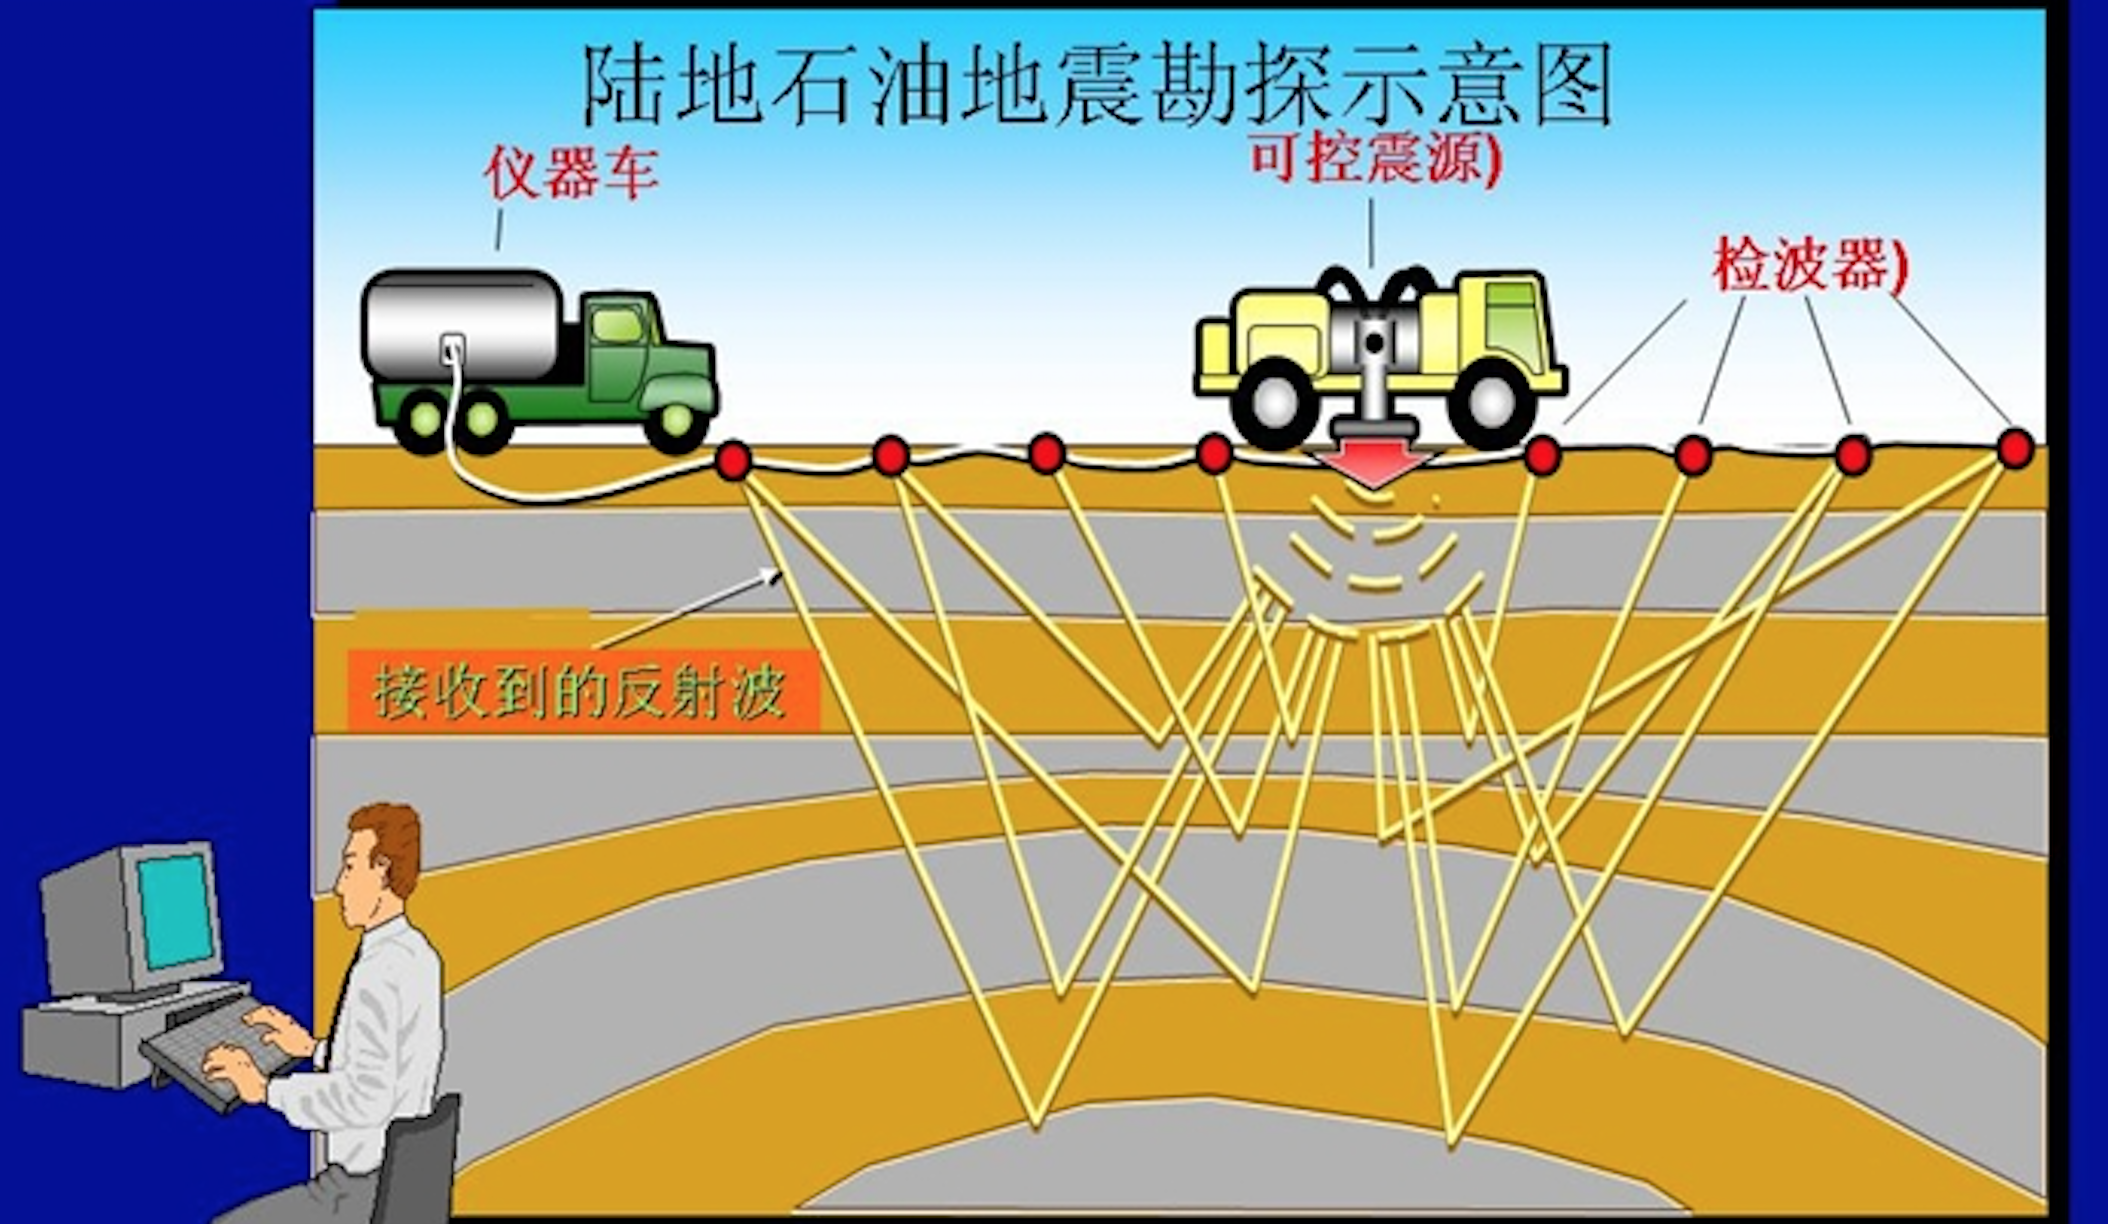
\includegraphics[width=\textwidth]{./Img/seismic2}
	\caption{地震波勘探模型.} \label{figure_seismic}
\end{figure}


由于反问题是高度线性不适定问题 \cite{hadamard1923lectures}, 换言之, 如果我们测量到的数据不准确或是有一个微小的扰动, 都会可能导致相对应的障碍物带来巨大的误差. 因此对反问题做适当形式的转化, 是求解反问题的重要方法. 类似于声波、电磁波, 弹性波反散射问题的方法主要也分为迭代法和直接成像法两种.  

迭代法是一种优化手段, 具体是将观察数据与初值参数构成目标函数, 然后将目标函数最小化的过程.  抽象为如下表达式:
\ben
\min_{\mathbf{m}} \ dist(\mathbf{d}^{obs},\mathbf{{L}}\mathbf{m}),
\een
其中 $\mathbf m$ 表示障碍物边界参数或是非均匀介质参数, $\mathbf{d}^{obs}$ 表示观测数据, $\mathbf{{L}}$ 表示弹性波方程的解算子, $dist(\cdot,\cdot)$ 表示某种距离. 
对于全空间弹性波障碍物散射问题, Li \cite{li2016inverse} 和 Bao \cite{bao2018direct} 提出了利用多频散射数据,基于区域导数的牛顿迭代法.  针对半空间非均匀弹性介质, Mora等人 \cite{mora1987nonlinear,feng2017elastic,elita2018elastic} 提出了最小二乘法反演介质参数的方法.  这些数值迭代方法的优势就是可以定量得到障碍物的边界或是介质参数信息, 但是要求一定的先验信息, 例如边界条件等.  由于每一次迭代都需要解一次弹性波正问题, 这无疑是相当巨大的计算量.  此外,这类优化问题一般都是非凸的, 这导致初值的选择, 迭代收敛性的证明都是比较困难的问题.  

直接成像法的基本思想是构造一个指示性成像函数,代入观测数据后, 该函数值在远离障碍物边界时逐渐衰减; 在靠近边界时, 函数值趋于峰值. 针对二维全空间弹性波反障碍物散射问题, Arens \cite{arens2001linear} 将线性采样法 (Linear Sampling Method) 从声波情形推广了到了弹性波情形.   Alves 和 Kress \cite{alves2002far}, Arens \cite{arens2001linear}, Charalambopoulos \cite{charalambopoulos2006factorization}, 以及  Hu, Kirsch \cite{hu2012some} 等发展了弹性波情形下的分解法 (Factorization Method) .  Ji 等 \cite{ji2018direct} 基于分解法提出了直接成像法,并证明了该函数在障碍物边界上有下界.  然而, 无论是线性采样法还是分解法, 至今都不能应用于弹性波反散射问题的近场数据. 这是因为, 我们没有办法将接收到的近场混合波数据分解成 p 波和 s 波, 除非我们能得到接收点附近领域内的所有数据.  Guzina 等
人 \cite{gintides2012identification} 利用拓扑导数方法对弹性波非均匀介质逆散射问题进行重构.  Chen 和 Huang \cite{ela_reverse} 针对全空间弹性介质扩展障碍物成像问题, 提出了单频加权弹性波逆时偏移方法,并且给出了弹性波逆时偏移方法的分辨率分析,该理论结果表明成像函数均为正值,从而保证了算法的稳定性. 

目前,在数学物理领域中, 对弹性波反散射问题的讨论主要集中于上述的全空间反障碍物散射问题,以及粗糙曲面反散射问题\cite{hu2016factorization,li2016near,liu2019near,hu2018direct},据本文作者所知,至今还极少有数学方面的文献来讨论半空间障碍物模型的.  然而,在地球物理领域中, 地震波勘探就是一个典型的半空间弹性波反散射模型.  因此, 本文将联系实际模型, 基于逆时偏移算法提出半空间弹性波反散射问题的直接成像法. 



\section{逆时偏移方法简介}

逆时偏移 (Reverse Time Migration) 是源于勘探地球物理领域的一种叠前深度偏移方法.  在逆时偏移流行之前, 单程波方程偏移法\cite{claerbout1972downward,gazdag1978wave} 一直是偏移研究的主要课题. 然而, 为了将波动方程分解成单程的上行波方程和下行波方程,需要引入平方根算子\cite{zhanggq1993,Zhang2007,zhang2018itoin}.  该平方根算子是一个拟微分算子,在数值计算时, 数值计算时需要用一系列的积分、微分算子来逼近,这给单程波方程的计算带来非常大的困难. 于是,基于全波方程的逆时偏移法在 1983年被 Whitmore \cite{whitmore1983iterative}, Baysal \cite{baysal1983reverse} 和 Mcmechan  \cite{mcmechan1983migration} 先后提出.  早期, 由于计算资源的匮乏, 工程师们把接收到的弹性波数据利用声波方程来进行逆时偏移 \cite{zhang2009,Zhang08,bleistein2013mathematics,claerbout1985imaging,berkhout2012seismic},但是由于弹性波是包含两种不同波数的 s 波和 p 波的耦合波, 两种波携带着不同的位移信息\cite{yan2008isotropic}.  因此, 发展利用弹性波全波方程的逆时偏移方法是必然的. Chang 和 McMechan \cite{chang1986reverse} 利用弹性波方程将接收到的弹性波数据时逆地外推到地表下, 然后提出了激励时间成像条件 (Excitation time), 而 Hokstad\cite{hokstad1998elastic} 利用 {Lam\'{e}} 势方法作为成像条件.  总之, 这两种成像条件都是互相关成像条件的特殊情形\cite{yan2008isotropic}. 此外, 由于弹性波包含 s 波和 p 波,地球物理学家发展出了两种基于 Helmholz 分解的逆时偏移算法 \cite{yan2008isotropic,sun2001scalar,denli2008elastic,chung2012implementation}.  

第一种方法是将接收到的弹性波数据,反传到接收面附近的浅层区域, 利用 Helmholtz 分解将耦合波场分解成 s 波向量势和 p 波标量势 \cite{etgen1988prestacked,zhe1997prestack}. 随后, 利用相应的 s 波波数与 p 波波数的声波方程将分解后的波正传回接收面. 最后利用传统的声波逆时偏移算法, 对分解完的数据分别进行相应波数的声波反传,随之与相应波数的声波点源互相关成像. 

第二种方法是先用弹性波全波方程将在表面接收到的位移数据反传到地下,然后将反传后的弹性波与点源发出的弹性波都进行波场分解, 最后对分解后的入射波与反传波作互相关\cite{dellinger1990wave}. 
 
总之, 逆时偏移算法的基本大致可以分成两步,第一步是将接收到的波数据作为在接收面上的 Dirichlet 边界条件,而后时逆地反传到背景介质中, 第二步是将入射波和反射波作互相关得出成像函数. 我们在此强调,本文中我们研究的逆时偏移算法不使用波场分解, 而是直接利用接收到的耦合的混合波场数据,经过反传后直接与入射波做互相关.  特别地, 我们的成像函数为 (详见 (\ref{cor2}) ):
\ben
\hat{I}_d(z)=\Im\sum_{q=e_1,e_2}\int_{\Gamma_0^d}\int_{\Gamma_0^d}\,
[\T_D(x_s,z)^Tq][\T_D(x_r,z)^T\overline{u^s_q(x_r,x_s)}]\,ds(x_r)ds(x_s).
\een
这里 $\Ga_0^d=\{x\in\Ga_0: x_1\in (-d,d)\}$, $d>0$, 是半空间表面接收数据的区间, $\T_D(x,z)$ 是 Dirichlet Green 函数在 $\Ga_0$ 上 $e_2$ 方向的应力张量 (详见 (\ref{DGT2}) ). 


关于逆时偏移方法的数学理论分析, 最早是由 Beylkin \cite{beylkin1984inversion,beylkin1985imaging,beylkin1990linearized} 基于广义 Radon 变换, 采用高
频渐近假设或者几何光学近似给出的渐近分析.  但是, 在实际的工程情况下, 这些假设的条件一般都不能满足. 近几年来, Chen 等\cite{chen2013reverse_acou,chen2013reverse_elec,thesis_guanghui} 针对全空间中声波和电磁波反障碍物散射问题, 研究了相应的单频逆时偏移方法来重构障碍物.  他们基于  Helmholtz-Kirchhoff 等式, 在不需要高频假设或几何光学近似的前提下,对算法的分辨率做出了严格分析, 并证明了该成像函数恒为正函数, 从而保证了该数值方法的稳定性. 在文献 \cite{chen2015reverse_planar} 中, Chen 等针对平行平板声波波导反散射问题,提出了基于逆时偏移算法的直接成像法. 在该文章中, 作者提出了广义的 Helmholtz-Kirchhoff 等式,并由此给出了成像分辨率的理论结果. 进一步, 文献\cite{RTMhalf_aco}中作者考虑声波半空间反散射问题的逆时偏移方法,并提出了全新的点扩散函数, 并且给出了分辨率的理论分析.  特别地, 该文章中给出了孔径选取的标准, 以及说明了半空间情形下只能对障碍物面向接收面的那部分进行成像, 这给本文的研究做了很好的铺垫. 

由于在实际的工程应用中, 获取观测数据的强度或振幅 (无相位数据) 比获取该观测数据的相位信息要容易很多. 由此, Chen等 \cite{chen2017phaseless,chen2016direct,chen2017direct,thesis_shaofeng} 基于逆时偏移算法,针对全空间声波,电磁波以及半空间声波反散射问题, 提出了无相位成像算法.  此外, 当障碍物远离发射面和接收面时, 证明了该无相位成像算法与原本的逆时偏移成像方法近似等价,并且给出了相应的误差分析. 




\section{本文内容安排}

本论文安排如下:

第二章中我们将介绍一些后文会涉及的函数空间,并且叙述后文会用到的经典的数学定理. 

第三章中我们利用 Fourier 变换推导出 Neumann Green 函数和 Dirichlet Green 函数, 并且研究 Green 函数的相关性质.  而后,通过极限吸收原理研究半空间弹性波散射问题解的适定性. 

第四章中我们首先介绍针对点源成像的点扩散函数, 然后提出重构半空间扩展障碍物的基于弹性波逆时偏移方法的直接成像法, 最后利用点扩散函数和散射系数逼近给出了该障碍物重构算法的分辨率分析. 

第五章中我们针对本论文中的研究进行总结, 并且叙述相关可待研究的问题. 


\chapter{基础知识}\label{chap:fundamental}
\section{函数空间}
我们首先引入后文需要用的记号和 Sobolev 空间 \cite{adams2003sobolev}. 令 $D$ 是 $\R^2$ 中的 Lipschitz 区域, 定义 $\Ga_D$ 是 $D$ 的边界.然后, 令 $L^2(D)$ 为 $D$ 上 Lebesgue 平方可积函数构成的 Hilbert 空间, 即
\ben
L^2(D)=\{u(x):\int_D|u|^2 dx<\infty\}.
\een
该空间的内积和范数定义如下:
\ben
<u,v>=\int_D u(x)\overline{v(x)} dx, \ \ \ \|u\|_{L^2(D)}=<u,u>^{1/2}.
\een
关于任意整数 $d\geq 0$, 可以定义 Sobolev 空间 $H^d(D)$ 为:
\ben
H^d(D)=\{u(x): \pa^\al u\in L^2(D), \ \ |\al|\leq d\},
\een
其中 $\al=(\al_1,\al_2)$, $\al_1,\al_2$ 为非负整数. 
当区域 $D$ 有界时, 我们引入如下 $H^1(D)$的加权范数:
\ben
\|u\|_{H^1({D})}=(\|\na \phi\|_{L^2({D})}^2+d_{D}^{-2}\|\phi\|_{L^2({D})}^2)^{1/2},
\een
其中 $d_D$ 是有界区域 $D$ 的直径. 进一步, 定义边界上的分数次 Sobolev 空间 $H^{1/2}(\Ga_{D})$ 为:
\ben
H^{1/2}(\Ga_{D})=\{v(x):  \|v\|_{L^2(\Ga_\mathcal{D})}<\infty, \ \ |v|_{\frac 12,\Ga_\mathcal{D}}<\infty      \},
\een
其中有:
\ben
|v|_{\frac 12,\Ga_\mathcal{D}}=\left(\int_{\Ga_\mathcal{D}}\int_{\Ga_\mathcal{D}}\frac{|v(x)-v(y)|^2}{|x-y|^2}ds(x)ds(y)\right)^{1/2}.
\een
且$H^{1/2}(\Ga_{D})$加权范数定义为:
\ben
\|v\|_{H^{1/2}(\Ga_{D})}=(d_{D}^{-1}\|v\|_{L^2(\Ga_{D})}^2+|v|_{\frac 12,\Ga_{D}}^2)^{1/2}.
\een
于是, 通过尺度变换技巧和迹定理,易得如下不等式估计 \cite[corollary 3.1]{RTMhalf_aco}
\begin{lem}
假设 D 是有界 Lipschitz 区域,	对于任意 $\phi\in C^1(\bar{D})^2$ 存在与 $d_{D}$ 无关的常数 $C>0$ ,成立如下不等式:
	\be\label{q0}
	\|\phi\|_{H^{1/2}(\Ga_{D})}+\|\sigma(\phi)\nu\|_{H^{-1/2}(\Ga_{D})}\le C\max_{x\in \bar{D}}(|\phi(x)|+d_{D}|\na\phi(x)|).
	\ee
\end{lem}

由于散射问题都是定义在无穷区域上的, 所以我们还需要定义无穷区域上的加权 Sobolev 空间. 假设 $\Om$ 是无界区域,定义加权 Lebesgue 平方可积函数空间 $L^{2,s}(\Omega)$ 如下:
\ben
L^{2,s}(\Om)=\{v \in L^2_{\rm loc}(\Om): (1+|x|^2)^{s/2}v \in L^2(\Om) \},
\een
且相应的范数为:
\ben
\| v \|_{ L^{2,s}(\Om)} = \left(\int_{\Om}(1+|x|^2)^{s}|v|^2 dx \right)^{1/2}.
\een
于是, 我们可以定义加权 Sobolev 空间 $H^{1,s}(\Om),s \in \R$ 为
\ben
H^{1,s}(\Om)=\{v(x): v(x)\in L^{2,s}(\Om) , \ \  \nabla v(x)\in L^{2,s}(\Om)   \},
\een 
且其相应的范数为
\ben
\| v \|_{ H^{1,s}(\Om)} = (\| v \|^2_{ L^{2,s} (\Om} + \| \nabla v \|^2_{ L^{2,s}(\Om)})^{1/2}.
\een 


在全文中,针对 Sobolev 空间 $X$, 为简便起见我们把向量值空间 $X^2$ 或是张量值空间 $X^{2\times 2}$ 仍然记作 $X$, 而且 $X, X^2, X^{2\times 2}$ 的范数统一表示成 $\|\cdot\|_X$.

\begin{definition}[Cauchy 主值]\label{def:pv}
	假设 $c\in [a,b]$ 是函数 $f(x)$ 的奇点, 且对于任意 $\ep>0$, $f(x)$ 在区间 $(a,c-\ep)$ 或 $(c+\ep,b)$ 上可积. 若如下极限存在且有限,
	\ben
	\lim_{\ep\to 0^+}\int_{a}^{c-\ep}f(x)dx+\int_{c+\ep}^{b}f(x)dx.
	\een
	则称该极限为 $\int_{a}^{b}f(x)dx$ 的 Cauchy 主值. 
\end{definition}

\section{基本定理}
\begin{lem}[H\"{o}lder 不等式]
	假设 $n$ 为正整数, 且 $p,q\in(1,+\infty)$ 满足 $\frac{1}{p}+\frac{1}{q}=1$, 则对于 $f\in L^p(\R^n)$ 和 $g\in L^q(\R^n)$ 成立如下不等式:
	\ben
	\|f\cdot g\|_{L^1(\R^n)}\leq\|f\|_{L^p(\R^n)}\|g\|_{L^q(\R^n)}.
	\een
\end{lem}
\begin{lem}[Parseval 等式]
  假设 $n$ 为正整数,对任意 $f, g \in L^2(\R^n)$, 定义 Fourier 变换 $\hat f(\xi)$ 为在范数$\|\cdot\|_{L^2_{\R^n}}$意义下的极限:
  \ben
  \hat f(\xi)=\lim_{R\to\infty}\int_{\|x\|\leq R}f(x)\ \ e^{-\i x\cdot \xi} dx.
  \een
  于是成立等式,
  \ben
  \int_{\R^n}f(x)\cdot \overline{g(x)}dx=
  \frac{1}{(2\pi)^n}\int_{\R^n}\hat f(\xi)\cdot \overline{\hat g(\xi)}d\xi.
  \een
  这里 $\overline{g(x)}$ 表示函数 $g(x)$ 的复共轭. 
\end{lem}

\begin{lem}[Betti 公式]
	假设 $D$ 为有界 Lipschitz 区域且其单位外法向为 $\nu$,对于 $u\in H^1(D)^2$ 和 $\Delta_e w\in L^2(D)^2$, 成立
	\ben
	\int_D u\cdot \Delta_e w dx =\int_{\pa D} u\cdot \sigma(w)\nu ds(x) -\int_D \ \lambda \ (\nabla\cdot u)(\nabla\cdot w)+2\mu \ \ep(u):\ep(w) dx,
	\een
	这里关于 $A=(a_{ij})$, $B=(b_{ij})$ , $i,j=1,2$, 有 $A:B=\sum_{i,j=1}^{2}a_{ij}b_{ij}$. 特别地, 如果进一步有 $\Delta_e u\in L^2(D)^2$, 则成立:
	\be\label{betti}
	\int_D u\cdot \Delta_e w-\Delta_e u \cdot w dx =\int_{\pa D} u\cdot \sigma(w)\nu -\sigma(u)\nu\cdot wds(x).
	\ee
\end{lem}
\chapter{半空间弹性波散射问题}\label{chap:Elastic}
正散射问题的研究一般包括 Green 函数的推导及其性质研究和散射解的适定性.  一般 Green 函数的推导都是通过对偏微分方程其中一个变量作 Fourier 变换后,得到常微分方程组, 然后结合基本解得出.  特别地, 二维弹性波方程的基本解 $\G(x,y)$ \cite{ku63} 为:
\be\label{Green}
\G(x,y)&=&\left(\frac{1}{\mu}g_{k_s}(x,y)  \I+\frac{1}{\om^2}\nabla\nabla g_{k_s}(x,y)\right)-\frac{1}{\om^2}\nabla\nabla g_{k_p}(x,y)\\
&:=&\G_s(x,y)+\G_p(x,y),
\ee
这里
\ben
g_{k}=\frac{\i}{4}\mathit{H}_0^{(1)}(k|x-y|)
\een
是波数为 $k$ 的 Helmholtz 方程的基本解 \cite{colton-kress}, 且 $\mathit{H}_0^{(1)}(t)$ 是零阶第一类 Hankel 函数 \cite{watson1995treatise}.  关于散射问题的适定性研究, 一般都是通过研究 Green 函数在无穷远处的渐近性质,然后据此推出辐射条件来保证方程的唯一性.  而存在性和稳定性一般是用变分方法或是边界积分法, 然后通过经典的 Riesz–Fredholm 理论 \cite{colton2013integral,kress1989linear} 结合唯一性得到.  然而由于横波和纵波在半空间表面初的耦合以及表面波的存在, 很难得出一个既保证唯一性又保证存在性的辐射条件.  因此,本文中我们不再依赖辐射条件,而是利用极限吸收原理 \cite{agmon1975spectral,Yves1988} 来得出方程的适定性. 在本章最后, 我们还将展示, 当障碍物远离半空间表面时, 其相应的散射解和在全空间情形下的散射解之间的关系. 

\section{半空间弹性波 Green 函数}\label{Green Tensor}
由于本文研究的正散射问题中, 弹性波需要在半空间表面 $\Ga_0$ 上满足 Neumann 边界条件 (\ref{eq2}), 所以我们先来研究满足 Neumann 边界条件的半空间 Green 函数.  之后, 由于逆时偏移算法中需要计算反传波, 因此我们还需要推导 满足 Dirichlet 边界条件的半空间 Green 函数及其 $e_2$ 方向的应力张量.

\subsection{Neumann Green 函数}\label{Neumann Green Tensor}
设源点$y\in\R^2_+$, 引入半空间弹性波Neumann零边界格林函数$\N(x,y)$, 对任意向量$q\in\R^2$, 其满足如下方程:
\be
& & \Delta_e [\N(x;y)q] + \omega^2 [\N(x,y)q] = -\mathbf{\delta}_y(x) q \ \ \mbox{in }\R^2_+ , \label{eq_n1} \\
& & \sigma(\N(x,y)q)e_2 = 0 \ \ \mbox{on } \Gamma_0, \label{eq_n2}
\ee
其中(\ref{eq_n2})代表该 Green函数满足半空间自由边界条件,${\delta}_y(x)$代表位于点y的Dirac源.  由于半空间的特性,我们将利用对$x_1$变量作Fourier变换的方式来推导Green函数,令
\be\label{a1}
\hat \N(\xi,x_2;y_2)= \int_\R\N(x_1,x_2;y) e^{-\i (x_1-y_1)\xi} dx_1,\ \ \forall \xi\in\C,
\ee
于是, 通过简单的推导计算, 对基本解 $\G(x,y)$ 的 $x_1$变量做Fourier变换后有
$\hat{\G}(\xi,x_2;y_2)=\hat{\G}_s(\xi,x_2;y_2)+\hat{\G}_p(\xi,x_2;y_2)$及
\be
& &\hat{\G}_s(\xi,x_2;y_2)=\frac{\i}{2\omega^2}
\left( \begin{array}{cc}
	\mu_s & -\xi\frac{x_2-y_2}{|x_2-y_2|} \\
	-\xi\frac{x_2-y_2}{|x_2-y_2|} & \frac{\xi^2}{\mu_s}
\end{array} \right)e^{\i\mu_s|x_2-y_2|}, \label{G1}\\
& &\hat{\G}_p(\xi,x_2;y_2)=\frac{\i}{2\omega^2} 
\left( \begin{array}{cc}
	\frac{\xi^2}{\mu_p} & \xi\frac{x_2-y_2}{|x_2-y_2|} \\
	\xi\frac{x_2-y_2}{|x_2-y_2|} & \mu_p
\end{array} \right) e^{\i\mu_p|x_2-y_2|},\label{G2}
\ee
这里$\mu_\alpha=(k_\alpha^2-\xi^2)^{1/2}$,$\alpha=s,p$, 其中 $k_p=\omega/\sqrt{\lam+2\mu}, k_s=\omega/\sqrt{\mu}$为p波和s波的波数. 
为了利用基本解$\G(x,y)$在 $x=y$ 处的奇性,我们令:
\ben
\N_c(x,y)=\N(x,y)-(\G(x,y)-\G(x,y')),
\een
其中$y'=(y_1,-y_2)$ 为y关于$x_1$轴的镜像点. 于是由式(\ref{eq_n1}-\ref{eq_n2}),可得$\N_c(x,y)$满足如下方程:
\be
& & \Delta_e [\N_c(x;y)q] + \omega^2 [\N_c(x,y)q] = 0 \ \ \mbox{in }\R^2_+ , \label{eq_n3} \\
& & \sigma(\N_c(x,y)q)e_2 =-\sigma(\G(x,y)-\G(x,y')) \ \ \mbox{on } \Gamma_0 . \label{eq_n4}
\ee
\begin{remark}
	在全篇论文中,我们假设对于任意的$z\in \mathbb{C}\backslash\{0\}$, $z^{1/2}$是多值函数$\sqrt{z}$ 的如下解析分支:$\Im(z^{1/2})\geq 0$,这对应于在复平面取右半实轴为割支线. 则对于$z=z_1+\mathbf{i}z_2$, $z_1,z_2\in\R$,
	\be \label{convention_1}
	z^{1/2}={\rm sgn}(z_2)\sqrt{\frac{|z|+z_1}{2}}+\i\sqrt{\frac{|z|-z_1}{2}},\ \ \forall z\in\C\backslash\bar{\R}_+.
	\ee
	当$z$位于右半实轴的上沿或是下沿时,取$z^{1/2}$为$\ep\rightarrow0^+$ 时$(z+\i\ep)^{1/2}$ 或是 $(z-\i\ep)^{1/2}$的极限即可. 
\end{remark}

通过对式(\ref{eq_n3}-\ref{eq_n4})两边作Fourier变换,我们得到关于变量$x_2$的常系数常微分方程组:
\be
 \mu \frac{d^2(e_1^T\hat \N_c q)}{dx_2^2}+\i(\lambda+\mu)\xi\frac{d(e_2^T\hat \N_c q)}{dx_2}+(\omega^2-(\lambda+2\mu)\xi^2)(e_1^T\hat \N_c q) = 0, \label{eq_n5}\\
 (\lambda+2 \mu)\frac{d^2(e_2^T\hat \N_c q)}{dx_2^2}+\i(\lambda+\mu)\xi\frac{d(e_1^T\hat \N_c q)}{dx_2}+(\omega^2-\mu \xi^2)(e_2^T\hat \N_c q) = 0. \label{eq_n6}
\ee
 由于我们要求$\N(x,y)$为外行波,因此方程 (\ref{eq_n5})的解可以表示成如下两个向量:
\ben
 \left[ \begin{array}{cc} \i\mu_s \\ -\i\xi \end{array} \right]e^{\i\mu_s x_2} \ , \ \ \ \ \ \left[ \begin{array}{cc} \i\xi \\ \i\mu_p \end{array} \right]e^{\i\mu_p x_2},
\een
的线性组合.  利用边界条件(\ref{eq_n6})及待定系数法,我们得到:
\be\label{NGT}
\hspace{-2cm}\hat \N_c(\xi,x_2;y_2) =  \frac{\i}{\omega^2\delta(\xi)}\sum_{\alpha,\beta=p,s}\mathbb{A}_{\al\beta}(\xi)e^{\i(\mu_\al x_2+\mu_{\beta} y_2)}, 
\ee
其中 $\varphi(\xi)=k_s^2-2\xi^2$, $\delta(\xi)=\varphi(\xi)^2+4\xi^2\mu_s\mu_p $, 以及 

\ben
&&{\mathbb{A}_{ss}(\xi)} =
\left( \begin{array}{ll}
	\varphi^2\mu_s & -4\xi^3\mu_s\mu_p \\
	-\xi\varphi^2  & 4\xi^4\mu_p
\end{array} \right),\ \ 
{\mathbb{A}_{sp}(\xi)} =
\left( \begin{array}{ll}
	2\xi^2\varphi\mu_s & -2\xi\varphi\mu_s\mu_p \\
	-2\xi^3\varphi  & 2\xi^2\varphi\mu_p
\end{array} \right),\\ 
\\
\\
&&
{\mathbb{A}_{ps}(\xi)} =
\left( \begin{array}{ll}
	2\xi^2\varphi\mu_s & 2\xi^3\varphi \\
	2\xi\varphi\mu_s\mu_p  & 2\xi^2\varphi\mu_p
\end{array} \right),\ \ 
{\mathbb{A}_{pp}(\xi)} =
\left( \begin{array}{ll}
	4\xi^4\mu_s & \xi\varphi^2 \\
	4\xi^3\mu_s\mu_p  & \varphi^2\mu_p
\end{array} \right).
\een

为了得到所需要的Neumann Green函数, 我们将对 $\hat{\N}(\xi,x_2;y_2)$ 做Fourier逆变换. 然而,根据如下引理所述, 函数$\delta(\xi)$在实轴上存在零点\cite{achenbach1980, Harris2001Linear},此时我们并不可以对其直接进行Fourier逆变换.
\begin{lem} \label{rayleigh}
	 Rayleigh方程 $\delta(\xi) = 0$在复平面$\C$中有且仅有两个根且记为 $\pm k_R$, 其中$k_R$满足$k_R>k_s$. 
\end{lem}

\debproof
 由前文注记中的(\ref{convention_1}), 易得 $\delta(\xi)$ 的割支线为 $C_l=\{\xi=\xi_1+\i\xi_2\in\C: \xi_1\in [-k_s,-k_p],\xi_2=0\}$ 和 
$C_r=\{\xi=\xi_1+\i\xi_2\in\C: \xi_1\in [k_p,k_s],\xi_2=0\}$. 于是$\delta(\xi)$在除 $C_l$ 和 $C_r$ 以外的区域解析.  而在割支线上,$\delta(\xi)$ 可表示成: 
\ben
\delta(\xi)=(k_s^2-2\xi^2)^2+\i\,[4\xi^2(k_s^2-\xi^2)^{1/2}(\xi^2-k_p^2)^{1/2}], \ \ \forall \xi\in C_l\cup C_r.
\een
显然, $\de(\xi)$ 在 $C_l\cup C_r$ 上没有零点.  又因为 $\de(\pm k_s)>0$ , $\de(\pm\infty)<0$ ,由函数的连续性得 $\de(\xi)$ 在区间 $(-\infty,-k_s)\cup(k_s,\infty)$ 上至少存在两个零点, 且由于其对称性,可以记为 $\pm k_R$.  下面, 我们将 $C_l, \ C_r$ 的上下沿分别记为 $C_l^\pm, \ C_r^\pm$. 

接下来, 利用幅角原理\cite{Ahlfors1979Complex}可以说明 $\delta(\xi)$ 在整个复平面只存在两个零点.  令 $\Ga_R$ 为半径 $R$ 充分大的圆. 我们考虑 $\mathcal D$ 是被周线 $\Ga_R$, $\Ga_l$ 以及 $\Ga_r$ 包围的区域.  其中 $\Ga_l$ 代表沿着 $C_l^+$ 从 $-k_s$ 到 $-k_p$  及然后沿着 $C_l^-$ 从 $-k_p$ 到 $-k_s$ ; 相应地, $\Ga_r$ 代表 沿着 $C_r^+$ 从 $k_p$ 到 $k_s$ 及然后 沿着 $C_r^-$ 从 $k_s$ 到 $k_p$ .  因为 $\delta(\xi)$ 在整个整个复平面上没有极点,  我们可以通过幅角原理来计算其在区域
 $\mathcal D$ 中的零点个数 $Z$ :
\be\label{zero}
Z=\frac{1}{2\pi\i}\int_C \frac{\delta'(\xi)}{\delta(\xi)}d\xi.
\ee
由式子(\ref{convention_1})中的定义,我们可以得出当$\xi\in C_r^\pm$时 $\de(\xi)=\de^\pm(\xi)$, 其中
\ben
\de^\pm(\xi)=(k_s^2-2\xi^2)^2\mp\i\,[4\xi^2(k_s^2-\xi^2)^{1/2}(\xi^2-k_p^2)^{1/2}\,]:=f_1(\xi)\mp\i f_2(\xi).
\een
于是可以有如下计算
\ben
\int_{\Ga_r} \frac{\delta'(\xi)}{\delta(\xi)}d\xi&=&\int_{k_p}^{k_s}\left(\frac{{\delta}_{+}' (\xi)}{\delta_{+}(\xi)}-\frac{{\delta}_{-}' (\xi)}{\delta_{-}(\xi)}\right) d\xi\\
&=&2\i\int_{k_p}^{k_s}\frac{f_1'(\xi) f_2(\xi)-f_1(\xi) f_2'(\xi)}{f_1^2(\xi)+ f_2^2(\xi)} d\xi\\
&=&-2\i\arctan \frac{f_2(\xi)}{f_1(\xi)}\Bigg|^{k_s}_{k_p}=0.
\een
相似地, 在 $\xi\in C_r^\pm$ 时也有 $\int_{\Ga_l}\frac{\delta'(\xi)}{\delta(\xi)}d\xi=0$ .  此外, 当 $|\xi|$ 足够大, 容易得到 $\de(\xi)$ 的渐近形式 $\delta(\xi)=-2(k_s^2-k_p^2)\xi^2+O(1)$   .  于是当 $R\gg 1$,可以计算得到
$\int_{\Ga_R} \frac{\delta'(\xi)}{\delta(\xi)}d\xi=4\pi\i$ . 
综上所述, 我们得出 $Z=2$ .  于是该引理得到证明. 
\finproof


为了克服上述问题,我们先假设半空间的介质是耗散的,然后研究其相应的Green函数,最后通过极限吸收原理得到$\N(x,y)$. 
记 $\mathbb{N}_{\omega(1+\i\ep)}(x,y)$ 为满足将式子(\ref{eq_n1})中将实圆频率$\omega$ 替换为复圆频率$\om(1+\i\ep)$后相应方程的Green函数.  同样的, 对$\mathbb{N}_{\omega(1+\i\ep)}(x,y)$关于$x_1$变量作Fourier变换,得到$\hat\N_{\omega(1+\i\ep)}(\xi,x_2;y_2)$,且通过相同的推导,其表达式与将(\ref{NGT})中将$k_s, k_p$替换为
$k_s(1+\i\ep), k_p(1+\i\ep)$后相应的式子一致.  下面的两个引理告诉我们,$\hat\N_{\omega(1+\i\ep)}(\xi,x_2;y_2)$的零点所在何处. 

\begin{remark}
	在本文中, 我们都假设耗散介质中所添加的 $\i\ep$ 是足够小的. 
\end{remark}
对于 $\al=s,p$, 令$\mu_{\al,\ep}(\xi)=((k_\al(1+\i\ep))^2-\xi^2)^{1/2}$. 于是, 根据规定 (\ref{convention_1}), 易得 $\mu_{\al,\ep}(\xi)$ 的割支线 $\mathcal{C_{\al,\ep}}$为
\ben
\mathcal{C_{\al,\ep}}&=&\{\xi=(\xi_1,\xi_2)\in\C \ | \ \Im \mu_{\al,\ep}(\xi)=0\} \\
&=&\{\xi=(\xi_1,\xi_2)\in\C \ | \   \xi_1\xi_2=k_\al^2\ep \ , \  \ \xi_2/\xi_1>\ep  \}.
\een
如图 \ref{figure_cut} 所示. 
\begin{figure}[htbp]
	\centering
	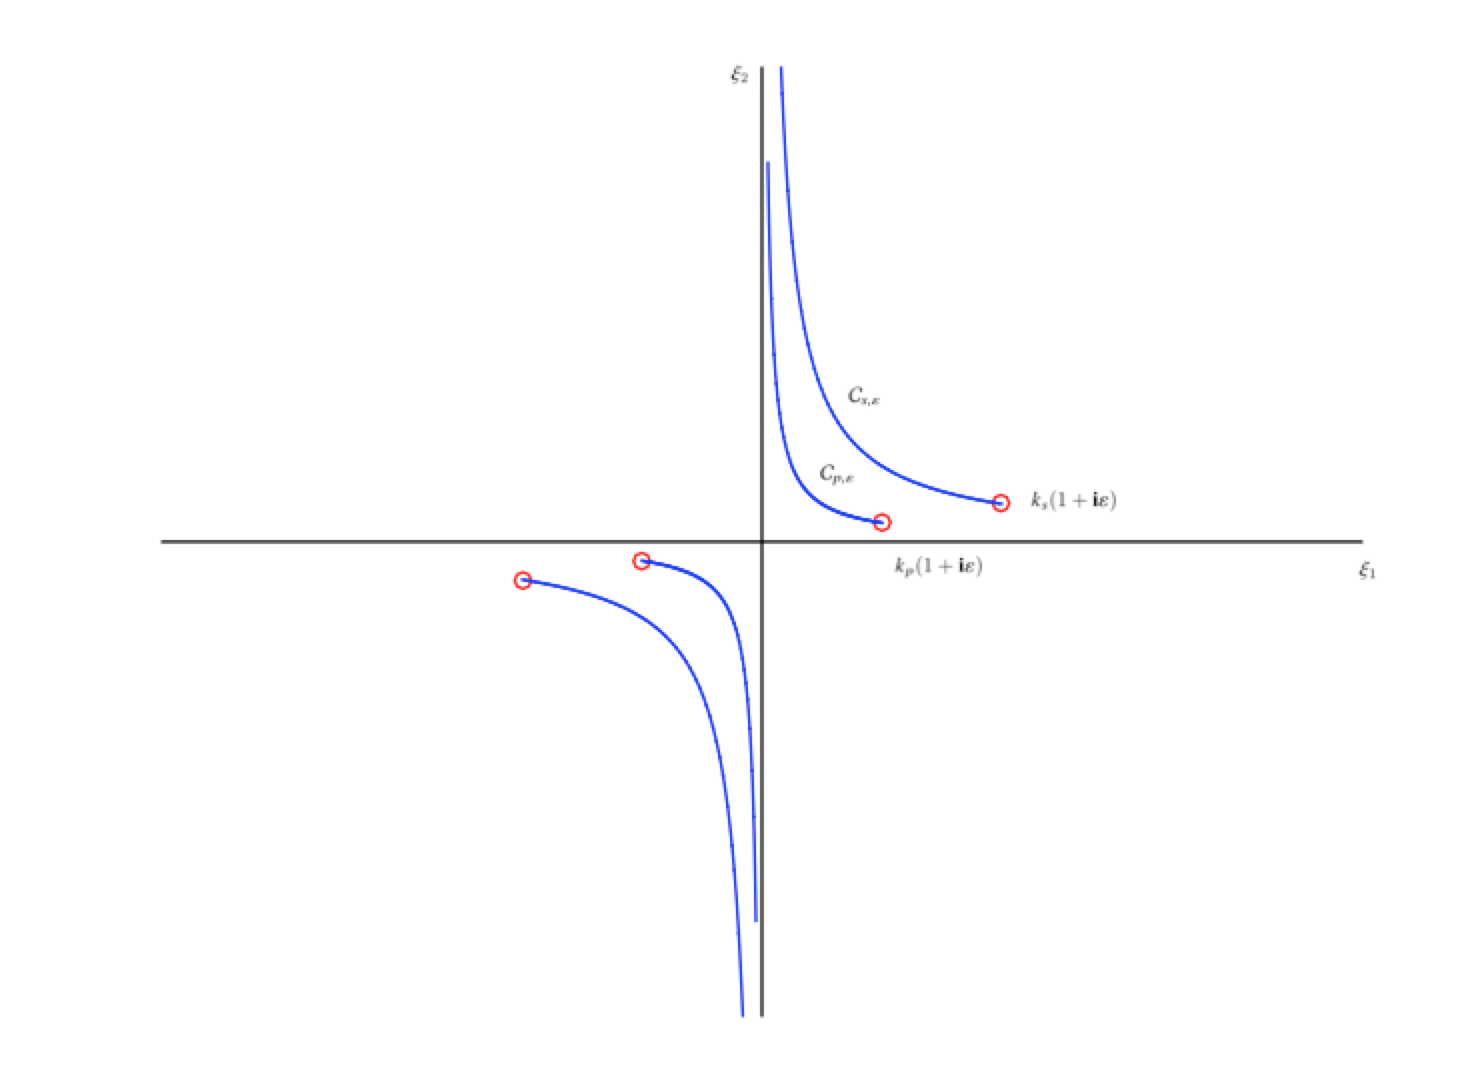
\includegraphics[width=\textwidth]{./Img/cut_plot}
	\caption{$\mu_{\al,\ep}(\xi)$, $\al=p,s$ 相应的割支线.} \label{figure_cut}
\end{figure}

令$\delta_{\om(1+\i\ep)}(\xi)$为将$\delta(\xi)$中的$k_p,k_s$替换成$k_s(1+\i\ep),  k_p(1+\i\ep)$后相应的复Rayleigh方程.  为了展现 $\delta_{\om(1+\i\ep)}(\xi)$ 的零点 与 $\delta(\xi)$ 的零点的关系,我们先来刻画在何种情况下可以结合或是分离根式 $z^{1/2}$ . 
\begin{lem}\label{lem23}
	令 $0<\ep<1$ , 假设 $z=R e^{\i\phi}$, $(1+\i\varepsilon)=r e^{\i\psi}$ 其中有 $0\leq\phi<2\pi$, $0<\psi<\pi/2$ 和  $R,r>0$. 于是等式
	\be
	z^{1/2}=(1+\i\varepsilon)(\frac{z}{({1+\i\varepsilon})^2})^{1/2}
	\ee
	成立当且仅当  $2\psi\leq\phi<2\pi$. 
\end{lem}
\debproof
令 
\ben
z_\ep=z/(1+\i\ep)^2:=R_\ep e^{\i\phi_\ep},
\een
 其中 $0\leq\phi_\ep<2\pi$. 于是,易得当 $2\psi\leq\phi<2\pi$ 时, 成立 
\ben
\phi_\ep=\phi-2\psi , \ R_\ep=R/r,
\een 
则有
\ben
z^{1/2}&=&\sqrt{R}e^{\i\phi/2}
=\sqrt{R/r}\sqrt{r}e^{\i(\phi/2-\psi)+\i\psi}\\
&=&\sqrt{R_\ep}\sqrt{r}e^{\i(\phi_\ep)+\i\psi}
=(1+\i\ep)z_\ep^{1/2}.
\een
同样地, 当 $0\leq\phi<2\psi$ 时, 成立 
\ben
\phi_\ep=\phi-2\psi+2\pi,
\een
 则有 
 \ben
 z^{1/2}=-(1+\i\ep)z_\ep^{1/2}.
 \een
  引理得证
\finproof

下面的引理告诉我们,$\hat\N_{\omega(1+\i\ep)}(\xi,x_2;y_2)$的零点所在何处. 

\begin{lem}\label{complex_rayleigh}
	复Rayleigh方程 $\delta_{\om(1+\i\ep)}(\xi)$在$\C\bks{\bar{\Om}}$中有且仅有两个根且为$\pm k_R(1+\i\ep)$.  其中集合$\Om$为
	\be\label{set:Om}
	\Omega := \{\xi_1+\i\xi_2 \in \mathbb{C} \ | \ k_p^2\ep<\xi_1\xi_2<k_s^2\ep \ , \  \ \xi_2/\xi_1>\ep\}.
	\ee
\end{lem}
\debproof
 我们定义 
 \ben
 \mu_\ep=(k^2(1+\i\ep)^2-\xi^2)^{1/2},k\in\R^+,
 \een
  令 
  \ben
& &  \xi=\xi_1+\i\xi_2,\xi_1,\xi_2\in\R, \ \ \  \\ & &(1+\i\varepsilon)=r e^{\i\psi}.
  \een
  通过简单的计算, 我们有
\be
\mu_\ep^2 &=& k^2(1-\ep^2)-\xi_1^2+\xi_2^2+\i(2k^2\ep-2\xi_1\xi_2)\\
&:=&Re^{\i\Theta} := a_1+\i a_2.
\ee
定义 $\Delta:=\{ \xi | 2\psi\leq\Theta<2\pi \} $ , 于是由引理 \ref{lem23}可知, 当 $\xi \in\Delta$ 时,成立
\ben
\mu_\ep = (k^2-\xi_\ep^2)^{1/2} (1+\i\ep),
\een
另一方面当 $\xi \notin\Delta$ 时,成立 
\ben
 \mu_\ep = - (k^2-\xi_\ep^2)^{1/2} (1+\i\ep),
 \een
 其中 $\xi_\ep=\xi/(1+\i\ep)$.  由于 $\ep$ 足够小, 我们可以有如下关于集合 $\Delta$ 的等价形式:
\be\nn
\Delta &=& (\pi/2\geq\Theta<2\pi)\cup(2\psi<\Theta<\pi/2) \\ \label{setd}
&=& \{ \xi | a_1 \leq 0 \} \cup \{ \xi | a_2 \leq 0 \} \cup \{ \xi | a_1 >0,a_2 >0 \ ,\ \ \tan\Theta \geq \tan(2\psi) \} \\ \nn
&:=& \Delta_1 \cup \Delta_2 \cup \Delta_3.
\ee
将 
\ben
& &a_1=k^2(1-\ep^2)-\xi_1^2+\xi_2^2, \\
& &a_2=(2k^2\ep-2\xi_1\xi_2).
 \een
  代入式子 (\ref{setd}) 中, 我们得到
\be
\Delta_1 &=& \{ \xi | \xi_1^2-\xi_2^2 \geq k^2(1-\ep^2) \},  \\
\Delta_2 &=& \{ \xi | \xi_1\xi_2 \geq k^2\ep \}.
\ee
又由于 $\tan\Theta=a_1/a_2$, $\tan\psi=\ep$, 易得
\be
\Delta_3 = \{ \xi | \xi_1^2-\xi_2^2 \leq k^2(1-\ep^2), \xi_1\xi_2 \leq k^2\ep ,
\frac{k^2\ep-\xi_1\xi_2}{k^2(1-\ep^2)-(\xi_1^2-\xi_2^2)} \geq \frac{\ep}{1-\ep^2} \}.
\ee
观察 $\Delta_3$ , 我们发现 $\Delta_3$ 表示成为 $\Delta_3=\Delta_{31}\cup\Delta_{32}\cup\Delta_{33}$ , 
其中
\ben
\Delta_{31} &=& \{ \xi | \xi_1\xi_2 \leq 0, 0\leq\xi_1^2-\xi_2^2 \leq k^2(1-\ep^2) \} ,\\
\Delta_{32} &=& \{ \xi |0 \leq \xi_1\xi_2 \leq k^2\ep, 0\leq\xi_1^2-\xi_2^2 \leq k^2(1-\ep^2), \frac{\xi_1\xi_2}{\xi_1^2-\xi_2^2} \leq \frac{\ep}{1-\ep^2} \}\\
&=& \{\xi | 0 \leq \xi_1\xi_2 \leq k^2\ep, 0\leq\xi_1^2-\xi_2^2 \leq k^2(1-\ep^2), \frac{\xi_2}{\xi_1} \leq \ep \}, \\
\Delta_{33} &=& \{ \xi |\xi_1\xi_2 \leq 0, \xi_1^2-\xi_2^2 \leq 0 ,\frac{\xi_1\xi_2}{\xi_1^2-\xi_2^2} \geq \frac{\ep}{1-\ep^2} \} \\
&=& \{ \xi |\xi_1\xi_2 \leq 0, \xi_1^2-\xi_2^2 \leq 0 ,-\frac{\xi_1}{\xi_2} \geq \ep \}.
\een
观察到 $\xi_1\xi_2 = k^2\ep$ , $\xi_1^2-\xi_2^2 = k^2(1-\ep^2)$ , $\xi_2=\xi_1\ep$ 三条曲线交于点 $\pm k(1+\i\ep)$, 于是区域 $\Delta$ 可以简化成:
\be
\Delta = \{\xi |-\frac{\xi_1}{\xi_2} \geq \ep, \ \frac{\xi_2}{\xi_1} \leq \ep\}\cup\{\xi | \xi_1\xi_2 \geq k^2\ep \}.
\ee
定义 $\Delta_s,\Delta_p$ 为将 $\mu_\ep$ 中的 $k$ 替换为 $k_s,k_p$ 后相应的 $\Delta$ 区域. 于是, 经过简单的整理, 我们可以得到:
\be
\overline{\C\bks\Omega} = (\Delta_s \cap \Delta_p )\cup (\overline{\C\backslash(\Delta_s \cup \Delta_p)}).
\ee
因此,当 $\xi\in\C\bks\Omega$ , 成立
\ben
\delta_{\om(1+\i\ep)}=\delta(\xi_\ep)(1+\i\ep)^4 .
\een
 通过引理 \ref{rayleigh} , 此引理得证. 
\finproof

 由引理\ref{complex_rayleigh} 我们得知 $\hat\N_{\omega(1+\i\ep)}(\xi,x_2;y_2)$ 在实轴上没有极点, 可以对其直接进行逆Fourier变换.  于是,半空间弹性波 Neumann Green函数 $\mathbb{N}(x,y)$ 可以利用极限吸收原理得到,即为
\be\nn
\N(x,y)&=&\lim_{\ep\to 0^+} \N_{\om(1+\i\ep)}(x,y)\\ \label{NGT1}
&=&\lim_{\ep\to 0^+}\frac{1}{2\pi}\int_\R\hat \N_{\om(1+\i\ep)}(\xi,x_2;y_2) e^{\i(x_1-y_1)\xi} d\xi.
\ee

现在, 我们已经得到 Neumann Green 函数的具体表达形式了.  但是,式子(\ref{NGT1})中这种极限形式并不利于我们分析该函数的具体性质,特别是其无穷远处的衰减阶数.  为了便于得到更加易于分析的表达形式, 我们引入下面这个关于柯西主值(cf. e.g. \cite[Chapter 4, Theorem 5]{Kuroda})的引理
\begin{lem}\label{cauchy_pv}
	令 $a,b\in\R,\  a<b$, 且 $t_0\in (a,b)$. 如果 $\gamma$ 在$[a,b]$上 H\"older 连续, 即存在常数 $\alpha\in (0,1]$ 及 $C>0$ 对于任意 $s,t\in [a,b]$, $|\gamma(s)-\gamma(t)|\le C|s-t|^\alpha$, 于是有
	\ben
	\lim_{z\to t_0,\pm\Im z>0}\int^b_a\frac{\gamma(t)}{t-z}dt={\rm p.v.}\int^b_a\frac{\gamma(t)}{t-t_0}dt\pm\pi\i\ga(t_0),
	\een
	其中 ${\rm p.v.}\int^b_a$ 表示积分的Cauchy主值. 
\end{lem}

通过引理 \ref{rayleigh}, 引理 \ref{complex_rayleigh} , 易知 $\hat\N_{\omega(1+\i\ep)}(\xi\mp k_R(1+\i\ep))$ 在点 $\pm k_R$ 的某个小邻域内解析且
关于 $\ep$ 一致有界.  于是, 对于足够小的 $d>0$,  成立:
\be
& &\lim_{\ep\to 0^+}\int_{\pm k_R-d}^{\pm k_R+d}\hat \N_{\om(1+\i\ep)}(\xi,x_2;y_2) e^{\i(x_1-y_1)\xi} d\xi \\
&=& \lim_{\ep\to 0^+}\int_{\pm k_R-d}^{\pm k_R+d}\frac{\hat \N(\xi,x_2;y_2)(\xi-k_R)}{\xi\mp k_R(1+\i\ep)} e^{\i(x_1-y_1)\xi} d\xi.
\ee
于是利用引理 \ref{cauchy_pv} , 表达式 (\ref{NGT1}) 及上面的等式, 我们就可以得到如下 Neumann Green 函数的表达式:
\be\label{NGT2}
\N(x,y)&=&\frac{1}{2\pi}\,{\rm p.v.}\int_{\R}\hat \N(\xi,x_2;y_2) e^{\i(x_1-y_1)\xi} d\xi\\
& &-\frac{1}{2\omega^2}
\left[\sum_{\alpha,\beta=p,s}\frac{\mathbb{A}_{\al\beta}(\xi)}{\de'(\xi)}e^{\i(\mu_\al x_2+\mu_\beta y_2)+\i(x_1-y_1)\xi}\right]^{k_R}_{-k_R},\ \ \forall x,y\in\R^2_+,
\ee
这里 $[f(\xi)]^b_a:=f(b)-f(a)$ . 

\begin{remark}
	值得注意的是, 由于 $\hat\N(\xi,x_2;y_2)$ 在实轴上存在极点,根据针对Green 函数的不同的研究目的, 最终$\N(x,y)$可以存在多种等价的表达形式.  例如, 在文献 \cite{nedelec2011} 中 Duran 等人是利用 Cauchy 积分定理以及留数定理将积分路径从实轴变换到双曲线上, 从而避开被积函数的极点.  可以证明的是, 本文中推导出的 Green 函数与文献 \cite{nedelec2011} 中的是一致的.  
\end{remark}
\begin{remark}
从 Neumann Green 函数的表达式 (\ref{NGT2})中,我们发现在其第二项中有 $\mu_{\al}(\pm k_R)=\i\sqrt{k_R^2-k_\al^2}$, 易知当 $x_2$ 增大时, 第二项的值是指数衰减的. 所以,式 (\ref{NGT2}) 中第二项对应的波只在 $\Ga_0$ 附近以波数 $k_R$ 传播,当远离 $\Ga_0$时非常微弱, 且称其为表面波 (或 Rayleigh 表面波) \cite{aki2002quantitative}. 
\end{remark}

为了后文分析的便利, 我们在以下引理中叙述若干关于 Rayleigh 函数 $\delta(\xi)$ 的性质. 

\begin{lem}\label{delta}
	令 $d_R=(k_R-k_s)/2$,其中 $k_R$ 为Rayleigh 表面波的波数. Rayleigh 函数 $\delta(\xi)$ 有如下性质: \\
	\rm{1}.对于任意 $|\xi|\le k_s+ d_R$, 存在只与 $\kappa$ 有关的常数 $C_1,C_2,C_3$,使得
	 \ben
	 & & C_1k_s^4\le |\delta(\xi)|\le C_2k_s^4, \\
	 & &|\delta^{(k)}(\xi)|\le C_3(|k_s^2-\xi^2|^{-k+1/2}+|k_p^2-\xi^2|^{-k+1/2}),  \ \ \ \ k=1,2  .
	 \een
	  \rm{2}. 对于任意 $|\xi|\geq k_R$, 存在只与 $\kappa$ 有关的常数 $C$,使得
	  \ben
	  |\de(\xi)|\ge Ck_s^2(|\xi|^2-k_R^2).
	  \een
	  \rm{3}. 
	  令$\de(\xi)=\de_1(\xi)(\xi^2-k_R^2)$, 对于任意 $k_R-d_R\le |\xi|\le k_R+d_R$, 存在只与 $\kappa$ 有关的常数 $C$,使得
	  \ben
	  |\de_1(\xi)|\ge Ck_s^2.
	  \een
\end{lem}

\debproof
利用简单的求导计算,我们易得结论1.  
通过 Rayleigh 函数的定义, 有 $|\xi|\ge k_s$, $\de(\xi)=k_s^4f({\xi^2}/{k_s^2})$, 其中
\ben
f(t)=(2t-1)^2-4t\sqrt{t-1}\sqrt{t-\kappa^2},\ \ \forall t\ge 1.
\een
对于任意 $t\geq 1$, 易得:
\be\nn
f'(t)&=&8t-4-4\sqrt{t-1}\sqrt{t-\kappa^2}-2t\sqrt{t-1}/\sqrt{t-\kappa^2}-2t\sqrt{t-\kappa^2}/\sqrt{t-1}\\ \label{df}
&\leq& 8t -4 -4\sqrt{t-1}\sqrt{t-k_R^2}-4t .
\ee
显然,当 $t\to1, \ t>1$ 时,$f'(t)\to-\infty$, 于是存在$\delta>0$ 以及 $A_1>0$, 使得当 $1<t<1+\delta$ 时, $f'(t)<-A_1$.  而当 $t\geq 1+\delta$ 时, 由式子 (\ref{df})得,存在 $A_2>0$ , 使得$f'(t)\leq -A_2$
又因为 $f(1)=1$ 以及 $f((2-\kappa^2)/(1-\kappa^2))<0$, 于是立得 $k_R^2\le\frac{2-\kappa^2}{1-\kappa^2}k_s^2$ .  然后由中值定理及 $f'(t)\leq -\max(A_1,A_2)$ 得
\ben 
\min_{|\xi|\ge k_s}\left|\frac{\de(\xi)}{\xi^2-k_R^2}\right|\ge\min_{t\geq1}|f'(t)|k_s^2\ge \max(A_1,A_2)k_s^2.
\een
结论2, 3得证. 
\finproof

观察式子 (\ref{G1}) , (\ref{G2}) , 及 (\ref{NGT}), 通过简单的变量替换, 我们易得 Neumann Green 函数满足如下对称性或是空间互易性,即
\be\label{symm}
\N(x,y)=\N(y,x)^T \ \ \ \ \ \ \ \forall x,y\in\R^2_+ \ .
\ee

而对于 $x_s\in\Ga_0$ 时的情况, 我们定义可以对应的 Neumann Green 函数 $\N(x,x_s),x\in\R^2_+$ 为 $\N(x,y)$ 在 $y\in\R^2_+,  \  y\to x_s$ 时的极限. 
由于半空间反散射问题中的点源一般都位于界面上, 所以接下去我们重点研究当 $x\in\Ga_0 ,  \ y\in\R^2_+$ 情形下的 Neumann Green 函数 $\N(x,y)$ . 
通过 (\ref{G1}) , (\ref{G2}) , (\ref{NGT}), 可以将 $\N(x,y)$ 简化为:
\be
\hat
\N(\xi,0;y_2)&=&\frac{\i}{\mu\delta(\xi)} \Bigg[ \Bigg(
\begin{array}{cc}
	2\xi^2\mu_s & -2\xi\mu_s\mu_p\\
	-\xi\varphi & \mu_p\varphi
\end{array} \Bigg)e^{\i\mu_p y_2} \\ \nn
& &
+ \Bigg(
\begin{array}{cc}
	\mu_s\varphi & \xi\varphi \\
	2\xi\mu_s\mu_p & 2\xi^2\mu_p
\end{array} \Bigg)e^{\i\mu_s y_2} \Bigg] \nonumber\\
&:=&\frac{1}{\delta(\xi)}(\Np(\xi)e^{\i\mu_p y_2}+\Ns(\xi)e^{\i\mu_s y_2}), \label{d2}
\ee
且当 $x\in\Ga_0, y\in\R^2_+$时,
\be\label{c8}
\N(x,y)&=&\frac{1}{2\pi}\,{\rm p.v.}\int_{\R}\hat \N(\xi,0;y_2) e^{\i(x_1-y_1)\xi} d\xi \\ \nn
& &+\frac\i 2
\left[\sum_{\al=p,s}\frac{\Na(\xi)}{\de'(\xi)}e^{\i\mu_\al y_2+\i(x_1-y_1)\xi)}\right]^{k_R}_{-k_R}.
\ee

为了便于研究 Neumann Green 函数在边界 $\Ga_0$上水平方向的渐近行为, 我们在下面引理中给出其更有便于分析的表达形式. 


\begin{lem}\label{lem:2.3} 令 $x\in\Ga_0 \ , y\in \R^2_+$ 以及 $\phi\in (-\pi/2,\pi/2)$ 且存在如下表达 $y_2=|x-y|\cos\phi \ ,
	x_1-y_1=|x-y|\sin\phi$ .  假设 $x_1\not= y_1$, 于是可以得到
	\be\label{NGT3}
	\N(x,y)&=&\frac{1}{2\pi}\int_L\mathbb{N}_0(t)\cos(t+\phi)e^{\i\lam\cos t}dt \\
	\nn
	& & \pm\i
	\left[\sum_{\al=p,s}\frac{\Na(\xi)}{\de'(\xi)}e^{\i\mu_\al y_2+\i(x_1-y_1)\xi}\right]_{\xi=\pm k_R},\label{h3}
	\ee
	其中 $\lam=k_s|x-y|$, $L$ 为复平面中的积分路径即 从 $-\pi/2+\i\infty$ 到 $-\pi/2$, $-\pi/2$ 再到 $\pi/2$, 接着从 $\pi/2$ 到 $\pi/2-\i\infty$ 的折线 ( 如图 \ref{figure_trans} 所示), 这里符号 $\pm$ 取决于 ${\rm sgn}(x_1-y_1)=\pm 1$, 且定义表达式:
	\be\label{h2}
	\mathbb{N}_{0}(t)=\sum_{\al=p,s}k_s\,\frac{\Na(k_s\sin(t+\phi))}{\de(k_s(\sin(t+\phi))}.
	\ee
\end{lem}

\debproof
不失一般性, 我们可以假设 $x_1>y_1$, 因此有 ${\rm sgn}(x_1-y_1)=1$.  注意到 $\hat{\N}(\xi,0;y_2)=\sum_{\al=p,s}\frac{\Na(\xi)}{\de(\xi)}e^{\i (y_2\mu_\al+(x_1-y_1)\xi)}$,所以对于 $\al=p,s$, 我们可以做经典的三角变量替换, 即为 $\xi=k_\al\sin t$ .  由于三角函数的周期性, 这里我们规定 $-\pi<\Re t \leq\pi$ 以保证变换的一一对应.  相应地, $\xi$ 在复平面中的积分路径 $\R$ 对应于 $t$ 所在复平面中的积分路径 $L$ .  于是得到如下等式:
\ben
& &\frac{1}{2\pi}\,{\rm p.v.}\int_{\R}\hat \N(\xi,0;y_2) e^{\i(x_1-y_1)\xi} d\xi \\
&=&\frac 1{2\pi}\,{\rm p.v.}\int_L\sum_{\al=p,s}k_s\,\frac{\Na(k_s\sin t)}{\de(k_s\sin t)}\cos t\, e^{\i \lam\cos (t-\phi)}dt.
\een
令 $L_{-\phi}$ 为 $L$ 平移 $-\phi$ 后的积分路径, 立即得到
\be\label{h1}
& &\frac{1}{2\pi}\,{\rm p.v.}\int_{\R}\hat \N(\xi,0;y_2) e^{\i(x_1-y_1)\xi} d\xi \\
&=&\frac 1{2\pi}\,{\rm p.v.}\int_{L_{-\phi}}\mathbb{N}_0(t)\cos (t+\phi)\,e^{\i\lam\cos t}dt,
\ee
这里 $\mathbb{N}_0(t)$ 如 (\ref{h1}) 所定义. 

设 $t_R\in L$ 满足等式 $k_R=k_s\sin t_R$, 于是 $k_R$ 即为 $t_R$ 在积分变换 $\xi=k_s\sin t$ 下的像点.  特别地, 由于 $k_R>k_s$, 则存在  $s_R>0$ 使得  $t_R=\pi/2-\i s_R\in L$ .  对于任意$\ep>0$,令 $ L^\ep$ 表示如下积分路径: \ben
& &-\pi/2+\i\infty\to -\pi/2+\i (s_R+\ep)\cup\pa B^+_\ep(-t_R)\\
&\to& -\pi/2+\i(s_R-\ep)
\to -\pi/2
\to\pi/2\to\pi/2-\i(s_R-\ep)\\
&\to&\pa B^+_\ep(t_R)\to\pi/2-\i(s_R+\ep)\to\pi/2-\i\infty,
\een
 其中 $\pa B^+_\ep(\pm t_R)$ 表示圆心在 $\pm t_R$ 半径为 $\ep$ 的右半圆  (如图 \ref{figure_trans} 所示).  然后, 令 $L^\ep_{-\phi}$ 为 $L^\ep$ 平移 $-\phi$ 后的积分路径.  于是, 利用 Cauchy 主值的定义及留数定理, 我们可以得知
\ben
& &\frac 1{2\pi}\,{\rm p.v.}\int_{L_{-\phi}}\mathbb{N}_0(t)\cos(t+\phi)\,e^{\i \lam\cos t}dt \\
&=&\lim_{\ep\to 0^+}\frac 1{2\pi}\int_{L^\ep_{-\phi}}\mathbb{N}_0(t)\cos (t+\phi)\,e^{\i \lam\cos t}dt\\
& &+\frac\i 2\sum_{t'=\pm t_R}{\rm Res}(\mathbb{N}_0(t)\cos (t+\phi)e^{\i \lam\cos t},t').
\een
\begin{figure}[htbp]
	\centering
	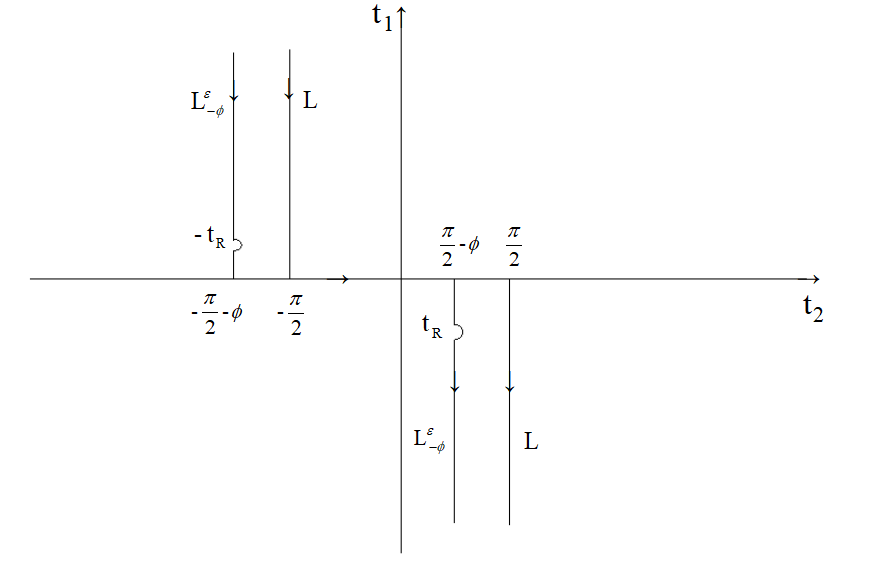
\includegraphics[width=\textwidth]{./Img/graphic/transformation4.png}
	\caption{ 积分路径 $L$ 和 $L^\ep_{-\phi}$.}\label{figure_trans}
\end{figure}
通过简单的计算, 易得相应留数为:
\ben
& &\frac\i 2\sum_{t'=\pm t_R}{\rm Res}(\mathbb{N}_0(t)\cos (t+\phi)e^{\i \lam\cos t},t')\\
&=&\frac \i 2\sum_{\xi=\pm k_R}\sum_{\al=p,s}\frac{\Na(\xi)}{\de'(\xi)}e^{\i (y_2\mu_\al+(x_1-y_1)\xi)}.
\een
另一方面,通过 Cauchy 积分定理, 我们得到 
\ben
& &\frac 1{2\pi}\int_{L^\ep_{-\phi}}\mathbb{N}_0(t)\cos (t+\phi)\,e^{\i \lam\cos t}dt \\
&=&\frac 1{2\pi}\int_{L}\mathbb{N}_0(t)\cos (t+\phi)\,e^{\i \lam\cos t}dt.
\een
最后利用 (\ref{c8}) 和 (\ref{h1}) 引理得证. 
\finproof
 
 上述引理是我们研究 Neumann Green 函数 $\N(x,y)$ 在界面 $\Ga_0$ 上当 $x\to\infty$ 时衰减行为估计的一个出发点.  下面, 我们先回顾下关于振荡积分衰减阶数估计的 Van der Corput 引理 \cite[P.152]{grafakos} . 
 
 \begin{lem}\label{van}
 	令 $\lam\ge 1$, $f\in C[a,b]$且其导函数绝对可积, 如果 $u\in C^k[a,b]$, 其中 $k\ge 1$ 及 $a<b$, 我们就有如下结论 \\
 	{\rm 1}. 如果 $|u'(t)|\ge 1$ 对于任意 $t\in (a,b)$ 成立,且 $u'$ 在 $(a,b)$ 上单调, 就断言
 	\ben
 	\left|\int^b_a f(t)e^{\i\lambda u(t)}dt\right|\le
 	3\lambda^{-1}\left(|f(b)|+\int^b_a |f'(t)|dt\right).
 	\een
 	{\rm 2}. 对于 $k\geq2$ 时, 如果 $|u^{(k)}(t)|\ge 1$ 对于任意 $t\in (a,b)$ 成立, 就断言 
 	\ben
 	\left|\int^b_a f(t)e^{\i\lambda u(t)}dt\right|\le
 	12k\lambda^{-1/k}\left(|f(b)|+\int^b_a|f'(t)|dt\right).
 	\een
 \end{lem}

在文献\cite{RTMhalf_aco}中,Chen 等对半空间逆时偏移算法进行研究时,引理 \ref{van} 起到了关键的作用. 该引理相对于驻相定理的优势在于,对于振幅函数 $f(t)$ 的光滑性要求更低,且对于 $\lambda$ 阶数的刻画具有一致性. 然而, 当振幅函数具有弱奇异点时,直接使用引理 \ref{van} 就行不通了.  幸运的是,经过研究,我们发现 当振幅函数存在弱奇异点, 且其与相位函数 $\phi(t)$ 的驻相点的距离存在正下界时, Van der corput 引理仍然成立,如下述引理刻画. 


\begin{lem}\label{lem:2.5}
	令 $\lam\ge 1$, 假设$f\in C[-\pi/2,\pi/2]$ 且其导函数绝对可积.  于是对任意区间 $(a,b)\subset (-\pi/2,\pi/2)$, 可以得到
	\be\label{c1}
	\left|\int_a^bf(t)e^{\i\lam\cos t}dt\right| 
	\leq C\lam^{-1/2}\left(|f(0)|+\int_a^b|f'(t)|dt\right),
	\ee
	这里常数 $C$ 与 $a,b,\lam$ 及被积函数 $f$ 无关.  
	此外, 令 $\kappa\in (0,1)$ 以及 $\phi\in (-\pi/2,\pi/2)$ 满足条件 $|\phi|\geq\phi^*>\arcsin \kappa:=\phi_\kappa$ , 可以得到
	\be\label{c3}
	 & &\left|\int_{-\frac\pi 2}^{\frac\pi 2}f(t)(\kappa^2-\sin^2(t+\phi))^{-1/2}e^{\i\lam\cos t}dt\right|  \\ \nn
	&\leq& C\lam^{-1/2}\left(|f(0)|+\int_{-\frac\pi 2}^{\frac \pi2}|f'(t)|dt\right),
	\ee
	这里常数 $C$ 只与 $\phi^*$ 和 $\kappa$ 有关. 
\end{lem}
\debproof
我们不妨假定 $\phi>0$ . 
其中估计 (\ref{c1}) 可以由引理 \ref{van} 直接得到.  这是因为区间 $(a,b)$ 可以被切割成若干个互不相交的子区间, 并且在任意一个子区间上面 $\sin t$ 单调且 $|\sin t|$ 存在下界 $1/\sqrt 2$ 或是 $|\cos t|$ 存在下界 $1/\sqrt 2$ . 

令 $g(t)=\kappa^2-\sin^2(t+\phi)$ .  由于 $0<\kappa<1$ $g(t)$, 易知 $g(t)$ 在区间 $(-\pi/2,\pi/2]$ 上有且仅有两个零点 $t_1, t_2$ , 而且可以求出
$t_1=\phi_\kappa-\phi$ 及 $t_2=-\phi_\kappa-\phi$ 或是 $t_2=\pi-\phi_\kappa-\phi$ , 这里 $t_2$ 取决于 $\phi+\phi_\kappa<\pi/2$ 或是 $\phi+\phi_\kappa\ge \pi/2$ .  不失一般性, 我在后面的证明中都假设 $t_2=\pi-\phi_\kappa-\phi$ . 

令 $0<\ep_0 <\min(\frac{\phi^*-\phi_\kappa}{2},\frac{\phi_\kappa}{2})$ .  显然成立 $t_1-\ep_0\geq -\pi/2, \ t_1+\ep_0\le -(\phi^*-\phi_\kappa)/2$ 以及 $t_2-\ep_0\ge(\phi^*-\phi_\kappa)/2$ . 于是, 我们可以把区间 $(-\pi/2,\pi/2)$ 切分成5个互补相交的子区间
\ben
& &I_1=(-\pi/2,t_1-\ep_0), \ I_2=(t_1-\ep_0,t_1+\ep_0), \\  
& &I_3=(t_1+\ep_0,t_2-\ep_0),  I_4=(t_2-\ep_0,t_2+\min(t_2+\ep_0,\pi/2)),\\ & &I_5=(\min(t_2+\ep_0,\pi/2),\pi/2).
\een
于是利用 (\ref{c1}) 可以得到
\be\label{c4}
& &  \left|\int_{I_1\cup I_3\cup I_5}f(t)(\kappa^2-\sin^2(t+\phi))^{-1/2}e^{\i\lam\cos t}dt\right| \\ \nn
&\leq& C\lam^{-1/2}\left(|f(0)|+\int_{-\frac\pi 2}^{\frac\pi 2}|f'(t)|dt\right),
\ee
其中常数 $C$ 只和 $\phi^*$ 及 $\kappa$ 有关.  

现在我们来估计在区间 $I_2, \ I_4$ 上的积分.  首先, 我们观察到, 在区间 $I_2\cup I_4$ 上成立不等式
 $|\sin t|\ge \sin((\phi^*-\phi_\kappa)/2)$ .  此外在该区间上还成立,
 \ben
 |g'(t)|=|\sin(2(t+\phi))|\ge \min(\sin\phi_\kappa,\sin(\phi^*+\phi_\kappa)).
 \een 
  令 $\de\in (0,\ep_0)$ 充分小,因为 $g(t_j)=0, j=1,2$, 于是利用中值定理, 对于任意 $t$ 满足 $ \de\le |t-t_j|\le \ep_0,j=1,2$ 我们有
\ben
\hspace{-1cm}|g(t)|\ge \min(\sin\phi_\kappa,\sin(\phi^*+\phi_\kappa))\de.\ \ 
\een
通过分部积分后,得到
\ben
& &\left|\int_{t_1-\ep_0}^{t_1-\de}f(t)g(t)^{-1/2}e^{\i\lam\cos t}dt\right| \\
&\le& C\delta^{-1/2}\lam^{-1}\left(|f(0)|+\int_{-\frac\pi 2}^{\frac \pi 2}|f'(t)|dt\right).
\een
类似地得到
\ben
& &\left|\int_{t_1+\de}^{t_1+\ep_0}f(t)g(t)^{-1/2}e^{\i\lam\cos t}dt\right| \\
&\le& C\delta^{-1/2}\lam^{-1}\left(|f(0)|+\int_{-\frac\pi 2}^{\frac \pi 2}|f'(t)|dt\right).
\een
最后,我们可以得到
\ben
& &\left|\int_{t_1-\delta}^{t_1+\de}f(t)g(t)^{-1/2}e^{\i\lam\cos t}dt\right| \\
&\leq&C\max_{t\in(-\pi/2,\pi/2)}|f(t)|\int_{-\delta}^{\de}|\kappa -\sin(\phi_\kappa+t)|^{-1/2}dt\\
&\leq&C\de^{1/2}\max_{t\in(-\pi/2,\pi/2)}|f(t)|.
\een
如此, 我们只要取 $\delta=\lam^{-1}$ 就可以得到
\ben
& &\left|\int_{I_2}f(t)(\kappa^2-\sin^2(t+\phi))^{-1/2}e^{\i\lam\cos t}dt\right| \\
&\leq& C\lam^{-1/2}\left(|f(0)|+\int_{-\frac\pi 2}^{\frac \pi 2}|f'(t)|dt\right).
\een
同理,在区间 $I_4$ 上的积分也可以被估计.  结合式子 (\ref{c4}) 中的估计, 引理得证. 

\finproof

\begin{lem}\label{lem:2.7}
	令 $\phi\in (0,\pi/2)$ 以及 $H$ 表示双曲线 
	\ben
	\{\xi=\xi_1+\i\xi_2\in\C:(\xi_1/(k_s\cos\phi))^2-(\xi_2/(k_s\sin\phi))^2=1\}.
	\een 
	定义 $f(\xi)$ 为 $H$ 邻域上的解析函数.  于是, 存在只与 $\kappa$ 有关的常数 $C$, 成立
	\ben
	& &\left|\int_{L\bks [-\pi/2,\pi/2]}f(k_s\sin(t+\phi))e^{\i\lam\cos t}dt\right|\\
	& &+\left|\int_{L\bks [-\pi/2,\pi/2]}f(k_s\sin(t+\phi))\cos te^{\i\lam\cos t}dt\right|\\
	\hskip-2cm&\le&C\lam^{-1}(|f(0)|+\max_{\xi\in H}(k_s|f'(\xi)|)).
	\een 
\end{lem}

\debproof
注意到, 对于 $t=-\pi/2+\i s$, $s>0$ 有 $k_s\sin(t+\phi)=-\cosh(s)\cos\phi+\i\sinh(s)\sin\phi\in H$ .  于是
\ben
I&= &\int_{-\pi/2}^{-\pi/2+\i\infty}f(k_s\sin(t+\phi))e^{\i\lam\cos t}dt\\
&=&\i\int^\infty_0f(-\cosh(s)\cos\phi+\i\sinh(s)\sin\phi)e^{-\lam\sinh(s)}ds.
\een
于是, 利用分部积分就可以得到
\ben
|I|&=&\left|\int^\infty_0f(-\cosh(s)\cos\phi+\i\sinh(s)\sin\phi) /(-\lam\cosh(s)) \ de^{-\lam\sinh(s)}\right| \\
&\leq&\lam^{-1}(|f(0)|+\int^\infty_0\left|\frac{df(-\cosh(s)\cos\phi+\i\sinh(s)\sin\phi)/\cosh(s))} {ds}\right|e^{-\lam\sinh(s)}ds).
\een
由此得到 $\pi/2\to\pi/2-\i\infty$ 上的积分值的估计.  于是, 不等式中的第一项估计得证.  类似地, 可以证明不等式中的第二项的估计.  引理得证. 
\finproof

经过前述若干引理的铺垫, 我们下面给出当 $x\in\Gamma_0$, $y\in\R_+^2$ 时, Neumann Green 函数相对于变量 $x_1$ 的阶数估计.  

\begin{thm}\label{es_NGT}
	假定 $x\in\Gamma_0$, $y\in\R_+^2$ 且满足 $|x_1-y_1|/|x-y|\ge(1+\kappa)/2$ 及 $k_sy_2\ge 1$ . 存在只与 $\kappa$ 有关的常数 $C$ , 使得如下估计成立:
	\ben
	|\N(x,y)|+k_s^{-1}|\na_y\N(x,y)|\leq \frac{C}{\mu}\left(\frac{k_sy_2}{(k_s|x-y|)^{3/2}}+e^{-\sqrt{k_R^2-k_s^2}y_2}\right).
	\een
\end{thm}

\debproof 这里我们只证明关于 $\N(x,y)$ 的估计.  由于 $\na_y\N(x,y)$ 的函数特性和  $\N(x,y)$ 一致, 同理可证.    由引理 \ref{lem:2.3} 中的式子 (\ref{h3}) 启发, 不失一般性, 我们假定 $x_1>y_1$ , 即有 $\phi\in (0,\pi/2)$ 且满足 
\ben
\phi\ge\phi^*=\arcsin (1+\kappa)/2>\phi_\kappa.
\een

 通过引理 \ref{delta} 中的结论 3 ,我们易得式子 (\ref{h3}) 中的第二项存在上界 $C\mu^{-1}e^{-\sqrt{k_R^2-k_s^2}y_2}$ , 即该项随着 $y_2$ 增大指数衰减. 

针对式子 (\ref{h3}) 中的第一项,我们将其分成 p 波和 s 波两项:
\ben
& &\frac 1{2\pi}\int_L\mathbb{N}_0(t)\cos(t+\phi)e^{\i\lam\cos t}dt\\
&=&
\frac 1{2\pi}\int_L\sum_{\al=p,s} k_s\frac{\Na(k_s\sin(t+\phi))}{\de(k_s\sin(t+\phi))}\cos(t+\phi)e^{\i\lam\cos t}dt.
\een
由于, p 波和 s 波在表达形式上是相似的, 这里我们只分析含有 $[\Np(k_s\sin(t+\phi))]_{22}=\mu^{-1}(\varphi\mu_p)(k_s\sin(t+\phi))$ 这项, 然后另一项的分析就同理可得.  为了表达简便, 我们有如下定义:
\ben
g(t)&=&k_s\frac{[\Np(k_s\sin(t+\phi))]_{22}}{\delta(k_s\sin(t+\phi))}\\
&:=&f(t)(\kappa^2-\sin^2(t+\phi))^{1/2}, \\ f(t)&=&\frac{k_s^2}{\mu}\frac{\varphi(k_s\sin(t+\phi))}{\de(k_s\sin(t+\phi))}.
\een
于是, 利用分部积分, 可以得到
\ben
& &\int_{L}g(t)\cos(t+\phi)e^{\i\lam\cos t}dt\\
&=&\cos\phi\int_Lg(t)\cos te^{\i\lam\cos t}dt-\sin\phi\int_{L}g(t)\sin te^{\i\lam\cos t}dt\\
&=&\cos\phi\int_Lg(t)\cos te^{\i\lam\cos t}dt-\frac{\sin\phi}{\i\lam}\int_{L}g'(t)e^{\i\lam\cos t}dt\\
&=&{\rm I}_1+{\rm I}_2.
\een
通过引理 \ref{delta} 中的结论 1 及引理 \ref{lem:2.5} 中的式 (\ref{c1}), 我们得到
\ben
& &\left|\int_{-\frac\pi 2}^{\frac \pi 2}g(t)\cos te^{\i\lam\cos t}dt\right|\\
&\le& C\lam^{-1/2}\left(|g(0)|+\int^{\frac\pi 2}_{-\frac\pi 2}|(g(t)\cos t)'|dt\right) \\
&\le& C\mu^{-1}\lam^{-1/2}.
\een
又因为 $\pm k_R$不在在双曲线 $H$ 上, 于是当 $\xi\in H$ 时, 成立
\ben
|[\Np(\xi)]_{22}|\le C|\xi|^3, \ \ 
|[\Np'(\xi)]_{22}|\le C|\xi|^2 , \ \
\de(\xi)\ge Ck_s^2|\xi|^2 .
\een
利用引理 \ref{lem:2.7} 我们得到
\ben
\left|\int_{L\bks [-\frac\pi 2,\frac\pi 2]}g(t)\cos te^{\i\lam\cos t}dt\right|\le C\mu^{-1}\lam^{-1}.
\een
于是得到 $|{\rm I}_1|\le C\mu^{-1}\lam^{-1/2}\cos\phi$ . 

 类似地,我们可以得到 $|{\rm I}_2|\le C\mu^{-1}\lam^{-3/2}$.  事实上,唯一的区别在于, 因为
\ben
g'(t)=f'(t)(\kappa^2-\sin^2(t+\phi))^{1/2}-f(t)(\kappa^2-\sin^2(t+\phi))^{-1/2}\sin(t+\phi)\cos(t+\phi),
\een
所以, 利用引理 \ref{lem:2.5} 中的  (\ref{c1}) 和 (\ref{c3}) 可以得到
\ben
\left|\int_{-\frac\pi 2}^{\frac \pi 2}g'(t)e^{\i\lam\cos t}dt\right|\le  C\mu^{-1}\lam^{-1/2}.
\een
于是, 我们最终得出
 \ben
 |{\rm I}_1+{\rm I}_2|&\le& C\mu^{-1}\lam^{-1/2}\cos\phi+C\mu^{-1}\lam^{-3/2}\\
 &\le& C\mu^{-1}(k_sy_2)/(k_s|x-y|)^{3/2},
 \een
  这里使用了条件 $k_sy_2\ge 1$.  引理得证. 
\finproof

从以上定理可以得知, $x\in\Gamma_0$, $y\in\R_+^2$ 时, Neumann Green 函数被两项控制, 其中第一项随着 $x_1$ 变大,以 3/2 阶衰减, 而第二项关于 $x_1$ 是常数, 但关于 $y_2$ 指数衰减. 值得注意的是, 弹性波基本解在横向关于 $x_1$ 是以 1/2 阶衰减的. 除了存在表面波, 该横向衰减性质也是弹性波 Neumann Green 函数与 声波 Neumann Green 函数本质不同的一个地方. 




\subsection{Dirichlet Green 函数}\label{Dirichlet Green Tensor}

由于相比于 Dirichlet Green 函数, Neumann Green 函数的形式更为复杂, 所以上一节中,我们先详细讨论了 Neumann Green 函数. 现在,我们可以类似且更加简单地来讨论 Dirichlet Green 函数 $\D(x,y), y\in\R^2_+$ \cite{arens1999}, 其满足如下方程及边界条件 
\be
& & \De_e [\D(x,y)q] + \omega^2 [\D(x,y)q] = -\mathbf{\de}_y(x)q \ \ \mbox{in } \R^2_+ , \label{eq_d1} \\
& &  \D(x,y)q = 0 \ \ \mbox{on } \Ga_0. \label{eq_d2}
\ee 

 类似于 (\ref{a1}) 中的频域 Neumann Green 函数 , 我们定义经过 Fourier 变换后的频域 Dirichlet Green 函数 $\hat{\D}(\xi,x_2;y_2)$.  经过类似地推导, 我们可以将它表达成如下形式:
\be\nn
\hat \D(\xi,x_2;y_2) &=& \hat \G(\xi,x_2;y_2)  -\hat \G(\xi,x_2;-y_2) \\
& &+ \frac{\i}{\omega^2 \gamma(\xi)}\sum_{\al,\beta=s,p}\mathbb{B}_{\al\beta}(\xi)e^{\i(x_2\mu_\alpha+y_2\mu_\beta)},\label{DGT}
\ee
这里有
\ben
& &\gamma(\xi)=\xi^2+\mu_s\mu_p , \ \mathbb{B}_{sp}(\xi)=-\mathbb{B}_{ss}(\xi), \ \mathbb{B}_{ps}(\xi)=-\mathbb{B}_{pp}(\xi),
\\
\\
& &{\mathbb{B}_{ss}(\xi)} =
\left( \begin{array}{ll}
	\xi^2\mu_s & -\xi\mu_s\mu_p \\
	-\xi^3  & \xi^2\mu_p
\end{array} \right),\ \ \ \ \ \
{\mathbb{B}_{pp}(\xi)} =
\left( \begin{array}{ll}
	\xi^2\mu_s & \xi^3 \\
	\xi\mu_s\mu_p  & \xi^2\mu_p
\end{array} \right).
\een
于是, 通过极限吸收原理, Dirichlet Green 函数 $\D(x,y)$ 可以看作是 $\D_{\om(1+\i\ep)}(x,y)$ 当 $\ep\to 0^+$ 时的极限 ,其中 $\mathbb{D}_{\omega(1+\i\ep)}(x,y)$ 为满足将式子(\ref{eq_d1})中将实圆频率$\omega$ 替换为复圆频率$\om(1+\i\ep)$后相应方程的Green函数. 
同样地, 对$\mathbb{D}_{\omega(1+\i\ep)}(x,y)$关于$x_2$变量的Fourier变换,得到$\hat\D_{\omega(1+\i\ep)}(\xi,x_2;y_2)$,且通过相同的推导,其表达式与将(\ref{DGT})中将$k_s, k_p$替换为
$k_s(1+\i\ep), k_p(1+\i\ep)$后相应的式子一致.  于是有:
\ben
\D(x,y)&=&\lim_{\ep\to 0^+} \D_{\om(1+\i\ep)}(x,y)\\
&=&\lim_{\ep\to 0^+}\frac{1}{2\pi}\int_\R\hat \D_{\om(1+\i\ep)}(\xi,x_2;y_2) e^{\i(x_1-y_1)\xi} d\xi.
\een
同样类似于 Rayleigh 方程, 关于 $\gamma(\xi)$ 有如下定理
\begin{lem} \label{root_Ga}
	令 $k_s,k_p\in \C$ 且有 $\Im(k_s)\geq0, \Im(k_p)\geq0$, 于是方程 $\gamma(\xi) = 0$ 在复平面中无零点. 
\end{lem}
\debproof
令 $F(\xi)= \gamma(\xi)*(\xi^2-\mu_s\mu_p)$ , 于是观察到 $\gamma(\xi) = 0$的根一定是 $F(\xi)=0$ 的根.  通过简单的计算, 可以得到 $F(\xi)=(k_s^2+k_p^2)\xi^2-k_p^2 k_s^2$ . 然而, 又易得当且仅当 $\xi_0^2=k_p^2 k_s^2 / (k_s^2+k_p^2)$, $F(\xi_0)=0$ 时, 有 $F(\xi)=0$.  但是此时 $\gamma(\xi_0)=2 k_p^2 k_s^2 / (k_s^2+k_p^2)$ . 
引理得证. 
\finproof
于是, 通过引理 \ref{root_Ga}及极限吸收原理, 我们得到如下 $\D(x,y)$ 的表达式:
\be\label{DGT1}
\D(x,y)&=&\G(x,y)-\G(x,y')\\
& &+\frac{\i}{2\pi\omega^2}\int_{\R}
\sum_{\al,\beta=s,p}\frac{\mathbb{B}_{\al\beta}(\xi)}{\ga(\xi)}e^{\i(\mu_\alpha x_2+\mu_\beta y_2)+\i(x_1-y_1)\xi}d\xi.
\ee
同样地,易得 Dirichlet Green 函数满足如下对称性或是空间互易性,即
\be\label{symm1}
\D(x,y)=\D(y,x)^T \ \ \ \ \ \ \ \forall x,y\in\R^2_+  \ .
\ee

由于我们的成像算法中, 需要对 $\Ga_0$ 上接收的数据反传, 这就需要用到 Dirichlet Green 函数 D(x,y) 的相关应力张量.  特别地, 我们针对 $x\in\Ga_0, y\in\R^2_+$, 定义 $\T_D(x,y)\in\C^{2\times 2}$ 为 Dirichlet Green 函数 $\D(x,y)$ 在 $e_2$ 方向的关于变量 $x_2$ 的应力向量 , 记为
\ben
\T_D(x,y)q=\sigma(\D(x,y)q)e_2, \forall q\in\R^2.
\een 
于是, 通过(\ref{DGT1}) 及求导计算, 我们得到
\be\label{DGT2}
\T_D(x,y)=\frac{1}{2\pi}\int_{\R}\hat \T_D(\xi,0;y_2) e^{\i(x_1-y_1)\xi}d\xi,\ \ \ \ \forall x\in\Ga_0,
\ee
其中 
\be\hspace{-1cm} 
\hat\T_D(\xi,0;y_2)&=&\frac 1{\gamma(\xi)}\left[\left(   \begin{array}{cc}
	\xi^2 & -\xi\mu_p \\
	-\xi\mu_s & \mu_p\mu_s
\end{array} \right)e^{\i\mu_p y_2}+
\left(   \begin{array}{cc}
	\mu_s\mu_p & \xi\mu_p \\
	\xi\mu_s & \xi^2
\end{array}\right)e^{\i\mu_s y_2}\right]\nonumber\\
\\
&:=&\Tp(\xi)e^{\i\mu_p y_2}+\Ts(\xi)e^{\i\mu_s y_2}.\label{d1}
\ee

下面的定理与定理 \ref{es_NGT} 相似, 其阐述了 $\D(x,y)$ 在 $\Ga_0$ 上的应力张量 $\T(x,y)$ 关于变量 $x_1$ 的衰减行为.  观察式子 (\ref{DGT2}), 我们发现与式子 (\ref{c8}) 相比它的形式更为简洁. 于是, 我们用类似于估计 $\N(x,y)$ 的方法, 即通过变量替换, 然后利用引理 \ref{lem:2.5} 及引理 \ref{lem:2.7}, 我们可以证明如下定理, 这里我们省略细节. 

\begin{thm}\label{es_DGT}
	令 $x\in\Gamma_0$, $y\in\R_+^2$ 满足 $|x_1-y_1|/|x-y|\ge (1+\kappa)/2$ 和 $k_s y_2\ge 1$ .  存在只与 $\kappa$ 有关的常数 $C$ 成立如下估计
	\ben
	|\T_D(x,y)|+k_s^{-1}|\na_y\T_D(x,y)|\leq C\frac{k_s^2 y_2}{(k_s|x-y|)^{3/2}}.
	\een
\end{thm}

\bigskip
观察定理 \ref{es_DGT}, 我们发现 $\T_D(x,y)$ 及其导数在 $x_1$ 增大时,其值关于 $x_1$ 是 3/2 阶衰减的, 这与声波 Dirichlet Green 函数的 $e_2$ 方向导数表现一致 \cite{RTMhalf_aco} . 特别地, 相比于文献\cite[Lemma 2.2]{arens1999}中对于该函数的估计,关于常数我们给出了更为准确的刻画, 即分子中的 $y_2$.  而且在 $\N(x,y )$ 中这种依赖于 $y_2$ 的表示估计, 对我们后面的算法分析是非常关键的. 
\begin{remark}
在这一节中, 我们注意到,在对 $\N(x,y)$ 或是 $\T_D(x,y)$ 的估计讨论时, 前提都需要满足条件 $|x_1-y_1|/|x-y|\ge (1+\kappa)/2$ .  这里我们作出说明: 第一,经过分析此条件是必要的, 该条件是为了保证振幅函数的弱奇异点与相位函数的稳相点不在同一点.  若我们去除此条件, 我们只能得到更弱的一致估计; 第二, 在后文分析中, 当需要用到 $\N(x,y)$ 或是 $\T_D(x,y)$ 的衰减性质时, 该假设条件都可以被满足.  
\end{remark}
\section{正散射问题解的适定性}

现在,我们将利用经典的极限吸收原理 (见文献 \cite{leis, wilcox1975, Yves1988}) 来定义半空间正散射问题的散射解. 假设 $D$ 为有界 Lipschitz 区域.  对于 $g\in H^{1/2}(\Ga_D)$,令 $\ep>0$ 以及 $u_\ep$ 满足如下方程
\be
& &\Delta_e u_\ep + [\omega(1+\i\ep)]^2 u_\ep =0 \ \ \mbox{\rm in } \R^2_+\bks \bar{D}, \label{pp3}\\
& &u_\ep= g \ \ \mbox{\rm on } \Ga_D, \ \ \ \ \\
& &\sigma(u_\ep)e_2=0 \ \ \mbox{\rm on } \Ga_0.  \label{pp4}
\ee
 由于上述方程中 $(1+\i\ep)$ 的存在, 将方程转化为变分形式后, 易得相应的双线性算子是有界且椭圆的, 于是由 Lax-Milgram 定理, 可以推出方程
 (\ref{pp3})-(\ref{pp4}) 在空间 $ H^1(\R^2_+\bks\bar D)$ 中存在唯一解 $u_\ep$ . 显然, 当 $s>1/2$ 时,成立 $u^\ep
 \in H^{1,-s}(\R^2_+\bks\bar D)$. 
 
为了后文表述方便, 我们引入如下双线性形式 $\GG(\cdot,\cdot)$:  即对于任意 $u,v\in H^1(\R^2\bks\bar D)$ 且满足 $\De_e u, \De_e v\in L^2(\R^2\bks\bar D)$, 令
\be\label{g1}
\GG(u,v)=\int_{\Ga_D} [u(x)\cdot \sigma(v(x))\nu- \sigma(u(x))\nu\cdot v(x)]ds(x).
\ee 
于是, 由于 $\N_{\om(1+\i\ep)}(x,y)$ 在无穷远处指数衰减,以及 $u^\ep(x)\in H^1(\R^2_+\bks\bar D)$, 利用 Betti 公式 (\ref{betti}) 易得 $u^\ep$ 的 Green 积分表达式,即对于任意 $q\in\R^2$ 有:
\be\label{gg2}
u^\ep(y)\cdot q=\GG(u^\ep(\cdot),\N_{\om(1+\i\ep)}(\cdot,y)q), \ \ \forall y\in\R^2_+\bks\bar D.
\ee

如果当$\ep\to 0^+$ 时, $u^\ep$ 在加权 Sobolev 空间$H^{1,-s}(\R^2_+\bks\bar D)$, $s>1/2$ 中存在极限 $u\in H^{1,-s}(\R^2_+\bks\bar D)$. 显然,$u$ 满足如下方程:
\be
& &\Delta_e u + \omega^2 u =0 \ \ \mbox{\rm in } \R^2_+\bks \bar{D}, \label{pp1}\\
& &u= g \ \ \mbox{\rm on }   \ \ \ \ \ \Ga_D, \ \ \ \ \\
& &\sigma(u)e_2=0 \ \ \ \ \ \ \mbox{\rm on } \Ga_0. \label{pp2}
\ee
由此我们定义 $u$ 为方程(\ref{pp1})-(\ref{pp2})的散射解. 
下面, 我们将说明 $u^\ep$ 在空间 $H^{1,-s}(\R^2_+\bks\bar D)$, $s>1/2$ 中,当 $\ep\to 0^+$时,一定存在极限. 首先,
定义微分算子 $-\De_e$ 的定义域为:
\ben
\mathcal{D}(\De_e,\R^2_+\bks\bar D)&=&\{v\in H^1(\R^2_+\bks\bar D): \De_e v\in L^2(\R^2_+\bks\bar D), \\
& &v=0\ \ \mbox{on }\Ga_D, \ \  \sigma(v)e_2=0\ \ \mbox{on }\Ga_0\}.
\een
 对文献 \cite{Yves1988}中的结果作适当的拓展, 我们可以得到如下结论:
 \begin{lem}\label{lap1}
 	若 $\om^2$ 不是算子 $-\De_e$ 在定义域 $\mathcal D(\De_e,\R^2_+\bks\bar D)$ 中的特征值, 则存在 $u\in H^{1,-s}(\R^2_+\bks\bar D)$ 当 $\ep\to0$ 时, $u_\ep$ 在空间  $H^{1,-s}(\R^2_+\bks\bar D)$ 中收敛到 u, 即
 	\ben
 	\lim_{\ep\to 0} \|u^\ep-u\|_{H^{1,-s}(\R^2_+\bks\bar D)}=0,
 	\een 
 	且 u 满足方程 (\ref{pp1})-(\ref{pp2}). 
 \end{lem}
根据引理 \ref{lap1}, 只需要证明算子 $-\De_e$ 在定义域 $\mathcal D(\De_e,\R^2_+\bks\bar D)$ 中不存在正特征值,就可以得到半空间障碍物散射问题的适定性.  在文献 \cite{sini2004} 中,Sini 针对半空间局部扰动问题证明了 
算子    $-\De_e$  在定义域 $\mathcal D'(\De_e,\Om)$ 中不存在正特征值,其中
   \ben
   \mathcal D'(\De_e,\Om)=\{v\in H^1(\Om), \ \De_e v\in L^2(\Om), \ \ \sigma(v)\nu=0\ \mbox{on }\Gamma_\Om \}.
   \een
   这里 $\Om\subset\R^2_+$ 是半空间 $\R^2_+$ 在边界 $\Ga_0$ 上局部扰动后的无界区域, $\Gamma_\Om$ 表示 $\Om$ 的边界, 且对于足够大的$R>0$, 满足
   \ben
   \{x\in\Om: \ \|x\|> R\}=\{x\in\R^2_+: \ \|x\|> R\}.
   \een

下面我们将 \cite{sini2004} 中的结果推广到半空间障碍物外问题,即算子
$-\De_e$ 在定义域 $\mathcal D(\De_e,\R^2_+\bks\bar D)$ 也不存在正特征值. 
\begin{lem}\label{2.1}\label{absence1}
	假设 $\om\in \R$ 以及 $u\in \mathcal{D}(\De_e,\R^2_+\bks\bar D)$ 满足如下方程: 
	\be\label{elastic_eq}
& &	\Delta_e u + \omega^2 u=0   \ \ \ \ \mbox{in } \ \ \ \R_+^2\bks \bar{D},\\ \label{elastic_bd}
& &	u=0 \ \ \ \ \ \ \ \mbox{on} \  \ \  \ \ \  \Ga_D , \ \ \\
& & \sigma(u)\cdot e_2=0 \ \ \ \ \ \mbox{on} \ \ \  \ \ \ \Ga_0 \ .
	\ee
	于是我们断言有 $u=0$. 
\end{lem}
在证明引理 \ref{absence1} 前, 我们先引入如下结果.  有了该结果可以发现上述定理中的边界条件 (\ref{elastic_bd}) 不是本质的, 当将其换成其它边界条件时,例如 Neumann 或是 阻抗边界条件, 引理 \ref{absence1} 依然成立. 

\begin{lem}\label{absence2}
	令函数 $f\in L^2(\R^2_+)$ 且有紧支集 $B\subsetneq \R\times(h,+\infty), \ h>0$.  假设 $\omega\in \R$ 以及 $u\in \mathcal{D'}(\De_e,\R^2_+)$ 满足如下方程:
	\be\label{eqq2}
	\De_e u +\om^2u = f.
	\ee
	我们断言在 $\mathcal{D'}(\De_e,\R\times(h,+\infty))$ 中 $u=0$. 
\end{lem}
\debproof
令 $\mathcal{F}_{x_1}(\cdot): L^2(R^2_+) \rightarrow L^2(R^2_+)$ 是针对单变量 $x_1$ 的 Fourier 变换, 即对于任意 $\xi\in \R$,
\ben
\hat{g}(\xi,x_2):=\mathcal{F}_{x_1}(g):=\int_\R g(x_1,x_2)e^{\i x_1\xi}dx_1.
\een
于是对于方程 (\ref{eqq2}) 两端作变换 $\mathcal{F}_{x_1}(\cdot)$ 后得到关于变量 $x_2\in R_+$ 的常微分方程组, 即对于任意 $\xi\in \R$ 有,
\ben
& & \mu \frac{d^2\hat u_1}{dx_2^2}+\i(\lambda+\mu)\xi\frac{d\hat u_2}{dx_2}+(\omega^2-(\lambda+2\mu)\xi^2)\hat u_1 =\hat{f_1} ,\\
& & (\lambda+2 \mu)\frac{d^2\hat u_2}{dx_2^2}+\i(\lambda+\mu)\xi\frac{d\hat u_1}{dx_2}+(\omega^2-\mu \xi^2)\hat u_2 = \hat{f_2} .
\een
以及在 $x_2=0$ 处的边界条件,
\ben
& & \mu\frac{d\hat u_1}{dx_2}+\i\mu\xi\hat u_2 = 0,\\
& & (\lambda+2\mu)\frac{d\hat. u_2}{dx_2}+\i\lambda\xi\hat u_1 = 0 .
\een
为了将上述方程组的系数变化成实数, 我们作如下函数替换:
\ben
v_1=\i \hat{u}_1 , \ \ \ \  v_2=\hat{u}_2,  \ \ \ \  \v=(v_1,v_2)^T, \\
q_1=\i \hat{f}_1 , \ \ \ \  q_2=\hat{f}_2,  \ \ \ \  \q=(q_1,q_2)^T.
\een
于是通过整理得到只含实系数的方程组:
\be\label{eq3}
& &[\A_1 \frac{d^2}{dx_2^2} +(\A_2-(\A_2)^T)\xi\frac{d}{dx_2}-\A_3\xi^2+\omega^2]\v=\q \ \ \ \ \ \mbox{in} \ \  \R_+ ,\\
& &(\A_1 \frac{d}{dx_2} +\A_2\xi) \ \ \v =0 \ \   \ \ \ \ \  \ \ \ \  \ \ \mbox{on} \ \ x_2=0.
\ee
其中 
\ben
\A_1=\Bigg( \begin{array}{cc}
	\mu &  0\\
	0 & \lambda+2\mu
\end{array} \Bigg) ,\ \  \ \ \
\A_2=\Bigg( \begin{array}{cc}
	0 & -\mu\\
	\lambda & 0
\end{array} \Bigg), \ \ \ \
\A_3=\Bigg( \begin{array}{cc}
	\lambda+2\mu &  0\\
	0 & \mu
\end{array} \Bigg).
\een
为了消去方程 (\ref{eq3}) 中的源函数 $\q$, 我们引入辅助函数 $\w$ 且其满足如下二次常微分方程组初值问题,
\ben
& &[\A_1 \frac{d^2}{dx_2^2} +(\A_2-(\A_2)^T)\xi\frac{d}{dx_2}-\A_3\xi^2+\omega^2]\w=\q \ \ \ \ \ \mbox{in} \ \  (0,h) ,\\
& &\w=0, \ \ \  (\A_1 \frac{d}{dx_2} +\A_2\xi) \ \ \w =0 \ \ \ \mbox{on} \ \  \ \ \ \ \ \ x_2=h.
\een
引入新的向量函数 $\W=(\w,(\A_1 \frac{d}{dx_2} +\A_2\xi) \w)^T$, $\Q=(0,0,\q)^T$, 可以将关于 $\w$ 的二次常微分方程组转化成关于 $\W$ 的一次常微分方程组,
\ben
& &\frac{d}{dx_2}\W = \A \W +\Q \ \ \ \ \ \mbox{in} \ \  (0,h), \\
& &\W=0  \ \ \ \mbox{on} \ \ \ \ \ \ \ \ \ x_2=h.
\een
其中 
\ben
\A=\left(
\begin{array}{cc}
	-\A_1^{-1}\A_2\xi & \A_1^{-1} \\
	-\A_2^T\A_1^{-1}\A_2\xi^2+\A_3\xi^2-\om^2 & \A_2^T\A_1^{-1}\xi
\end{array}
\right).
\een
利用针对常系数一次常微分方程组的标准理论, 我们可以得到,
\ben
\W(\xi,x_2)=-\Phi(\xi,x_2) \int_{h}^{x_2} \Phi^{-1}(\xi,t)\Q(\xi,t)dt,
\een
其中
\ben
\Phi(\xi,t)=\left(\begin{array}{cccc}
	-\mu_s(\xi) e^{\i \mu_s(\xi) t} & -\xi e^{\i\mu_p(\xi) t} & -\mu_s(\xi) e^{-\i \mu_s(\xi) t} & \xi e^{-\i\mu_p(\xi) t}  \\
	-\i \xi e^{\i \mu_s(\xi)(\xi) t} & \i\mu_p(\xi) e^{\i\mu_p(\xi) t} & \i \xi e^{-\i \mu_s(\xi) t} & \i\mu_p(\xi)  e^{-\i\mu_p(\xi) t} \\
	-\i\mu\beta(\xi) e^{\i \mu_s(\xi) t} & -2\i\mu \xi\mu_p(\xi)  e^{\i\mu_p(\xi) t} & \i\mu\beta e^{-\i \mu_s(\xi) t} & -2\i\mu \xi\mu_p(\xi)  e^{-\i\mu_p(\xi) t} \\
	2\mu \xi \mu_s(\xi) e^{\i \mu_s(\xi) t} & -\mu \beta(\xi)  e^{\i\mu_p(\xi) t} & 2\mu \xi \mu_s(\xi) e^{-\i \mu_s(\xi) t} & \mu \beta(\xi)   e^{-\i\mu_p(\xi) t}
\end{array}\right).
\een
\\
下面, 我们将 $\w(\xi,x_2)$ 在区间 $(h,\infty)$ 上延拓为零.  易得 $\w(\xi,x_2)$ 在关于 $x_2\in\R_+$ 满足方程组 (\ref{eq3}). 
因此,由 $\mu_p(\xi)$ 和 $\mu_s(\xi)$ 的性质及引理 \ref{rayleigh}, 易得 对于任意 $t\geq0$ 有 
$\Phi(\xi,t)$ 及 $\Phi(\xi,t)^{-1}$ 关于 $\xi$ 在 $\R\bks\{\pm k_p,\pm k_s,\pm k_R\}$ 中实解析, 即在 $\R\bks\{\pm k_p,\pm k_s,\pm k_R \}$ 中任一点的某个小邻域内函数都存在 Taylor 级数展开.  又因为 $f(x)$ 存在紧支集, 我们可以推出关于几乎所有的 $\xi\in \R$,  $\w(\xi,x_2), \ x_2\geq 0$ 实解析. 同理 $(\A_1 \frac{d}{dx_2} +\A_2\xi) \w$ 也具有该性质. 



令 $\UU=\v-\w$ 且表示为 $\UU=(U_1,U_2)^T$.  于是, 易得 $\UU$ 满足如下方程组:
\be\label{eq4}
& &[\A_1 \frac{d^2}{dx_2^2} +(\A_2-(\A_2)^T)\xi\frac{d}{dx_2}-\A_3\xi^2+\omega^2]\UU=0 \ \ \ \mbox{in} \ \ \  x_2\in\R_+ ,\\
& &(\A_1 \frac{d}{dx_2} +\A_2\xi)  \UU =(\A_1 \frac{d}{dx_2} +\A_2\xi)    \w \ \ \ \ \ \ \ \mbox{on} \ \ x_2=0. \label{bd2}
\ee
又因为上述方程组的系数相对于变量 $x_2$ 是常数,于是可以得到 $\UU(\xi,x_2)$ 有如下表达形式,
\ben\hspace{-2.5cm}
\UU(\xi,x_2)&=&c_1(\xi)\left(\begin{array}{l}
	-\mu_s \\
	-\i \xi
\end{array}\right)e^{\i \mu_s x_2}+c_2(\xi)\left(\begin{array}{l}
	-\xi \\
	\i \mu_p
\end{array}\right)e^{\i \mu_p x_2}\\
& &+c_3(\xi)\left(\begin{array}{l}
	-\mu_s \\
	\i \xi
\end{array}\right)e^{-\i \mu_s x_2}+c_4(\xi)\left(\begin{array}{l}
	\xi \\
	\i \mu_p
\end{array}\right)e^{-\i \mu_p x_2}.
\een

当 $\xi^2\leq k^2_p$ 时, 易得在 $L^2_{x_2}(\R_+)$ 中有 $\UU=0$ .  因此, 由边界条件 (\ref{bd2}) 易得当 $\xi^2\leq k^2_p$ 时 ,
\ben
(\A_1 \frac{d}{dx_2} +\A_2\xi)   \w|_{x_2=0} =0.
\een
于是由 $(\A_1 \frac{d}{dx_2} +\A_2\xi)   \w|_{x_2=0}$
 关于几乎所有的 $\xi \in \R$ 解析及边界条件 (\ref{bd2}) 我们可以推出, 关于几乎所有的 $\xi \in \R$,成立
\be\label{bd_1}
(\A_1 \frac{d}{dx_2} +\A_2\xi)  \UU =0  \ \ \ \ \ \mbox{on} \ \ \ x_2=0.
\ee
进一步, 当 $\xi^2>k^2_p$, $\UU\in L^2_{x_2}(\R_+)$ 存在如下形式,
\ben
\UU(\xi,x_2) = \left\{
\begin{array}{l}
	c_0(\xi)\left(\begin{array}{l}
		-\xi \\
		\i \mu_p
	\end{array}\right)e^{\i \mu_p x_2},     \ \ \ \ \   k_p^2<   \xi^2\leq k_s^2 , \\
	c_1(\xi)\left(\begin{array}{l}
		-\mu_s \\
		-\i \xi
	\end{array}\right)e^{\i \mu_s x_2}+c_2(\xi)\left(\begin{array}{l} 
		-\xi \\
		\i \mu_p
	\end{array}\right)e^{\i \mu_p x_2}, \ \ \xi^2>k_s^2
\end{array}.
\right. 
\een
于是有
\ben 
(\A_1 \frac{d}{dx_2} +\A_2\xi)  \UU = \left\{
\begin{array}{l}
	c_0(\xi)\left(\begin{array}{l}
		-2\i\mu\xi\mu_p \\
		-\mu\beta
	\end{array}\right)e^{\i \mu_p x_2},     \ \ \ \ \   k_p^2<   \xi^2\leq k_s^2,  \\
	c_1(\xi)\left(\begin{array}{l}
		-\i\mu\beta \\
		2\mu\xi\mu_s
	\end{array}\right)e^{\i \mu_s x_2}+c_2(\xi)\left(\begin{array}{l} 
		-2\i\mu\xi\mu_p \\
		-\mu\beta
	\end{array}\right)e^{\i \mu_p x_2}, \ \ \xi^2>k_s^2
\end{array}.
\right. 
\een
因此, 利用条件 (\ref{bd_1}), 易得 $c_0(\xi)=0$  和

\be
\mathbf{det} \left(\begin{array}{ll}
	-\i\mu\beta & -2\i\mu\xi\mu_p \\
	2\mu\xi\mu_s &	-\mu\beta
\end{array}\right)=-\i\mu(\beta^2+4\xi^2\mu_s\mu_p)=0
\ \ \ \  \mbox{for} \ \ \xi^2>k_s^2.
\ee
 利用引理 \ref{rayleigh},易得当$\xi\neq\pm k_R$ 时 $c_1(\xi)=c_2(\xi)=0$ . 于是, 关于几乎所有的 $\xi\in\R$ 及 $x\in \R^+$, 成立$\UU(\xi,x_2)=0$. 由于 $\v=\UU+\w$, 易知关于几乎所有的   $\xi\in\R$ 及 $x_2\in(h,+\infty)$ 成立 $\v(\xi,x_2)=0$.  于是通过将 $\hat{\u}(\xi,x_2)$ 作逆 Fourier 变换,引理得证. 
\finproof



{\noindent \bf 引理 \ref{absence1} 的证明:} 

由于 $D\subsetneq\R^2_+$, 我们可以找到半径分别为 $R_1$ 和 $R_2$ 的同心圆 $B_{R_1},B_{R_2}$ 且满足关系式 $D\subsetneq B_{R_1}\subsetneq B_{R_2}  \subsetneq \R^2_+$.  令 $\chi \in C_{0}^{\infty}(\R^2_+)$ 是一截断函数, 且满足 $0 \leq \chi \leq 1$,当$x\in B_{R_1}$ 时 $\chi=0$  以及当 $x\notin \overline{B_{R_2}}$ 时 $\chi=1$. 

进一步, 我们定义 $v=\chi u$,
易得 $v$ 满足方程 (\ref{eqq2}), 且其中
\ben
f=\sigma(u)\na\chi+(\lambda+\mu)(\na^2 \chi u+ \na u \na\chi)+\mu\Delta\chi u +\mu\div u\na\chi,
\een
 这里 $\na^2 \chi$ 是 $\chi$ Hessian 矩阵.  显然成立 $f\in L^2(\R^2_+)$ 且存在紧支集.  因此, 利用引理 \ref{absence2}, 可以得到存在足够大的 $h>0$, 当 $x\in \R\times(h,+\infty)$ 时, $u=v=0$.  最后,利用弹性波方程的唯一延拓性原理 \cite{Morassi2001STRONG},
立得在 $\R^2_+$ 中, u=0 .  引理得证. 
\finproof

利用相似的理论推导, 上述结果可以推广到可穿透障碍物情形,即有如下定理,
\begin{lem}
	假设 $\om\in \R$ 以及 $u\in \mathcal{D}(\De_e,\R^2_+)$ 满足如下方程: 
	\ben
	\De_e \u + \om^2 (1+n(x)) \u =0,
	\een
	这里 $n(x)\in L^{\infty}(D)$ 是一个在 $D$ 存在紧支集的正标量函数,
	于是我们断言有 $\u=0$.
\end{lem}


现在, 我们利用引理 \ref{lap1} 和引理 \ref{absence1}, 易得如下半空间弹性波散射问题解的适定性. 
\begin{thm} \label{thm:4.1}\label{lap2}
	对于任意 $g \in H^{1/2}(\Ga_D)$, 半空间散射问题 (\ref{pp1})-(\ref{pp2})
	存在唯一的散射解 $u\in H^{1}_{\rm loc}(\R^2_+ \backslash \bar D)$. 此外, 对于任意有界区域 $\mathcal O\subset \R^2_+\bks\bar D$ 存在常数 $C>0$ 成立如下估计:
	\ben
	\|u\|_{H^{1}(\mathcal O)}\le C\|g\|_{H^{1/2}(\Ga_D)}.
	\een
\end{thm}

关于半空间散射问题在其它边界条件的情形或是对于可穿透障碍的情形, 以上论证都可以类似推广到相应情形. 利用 $u^\ep$ 的 Green 表示公式 (\ref{gg2}), 令 $\ep\to 0$, 可以得到关于半空间弹性波问题散射解 $u$ 的 Green 表示公式: 
\be\label{g2}
u(y)\cdot q=\GG(u(\cdot),\N(\cdot,y)q), \ \ \forall y\in\R^2_+\bks\bar D,\ \ \forall q\in\R^2.
\ee
\begin{remark}
	我们针对散射解做一说明,在通篇全文中提到的散射解, 无论方程建立在哪种背景介质或是无界区域 $\Om
	$ 内,散射解 $u$ 都是指将原方程中的角频率 $\om$ 替换成 $\om(1+\i\ep)$ 后得到相应方程的解 $u^\ep$ 在空间 $H^{1,-s}(\Om)$, $s>1/2$ 中的极限. 特别地, 利用极限吸收原理得到的全空间散射问题的散射解 \cite{leis, cxz2016} 与所谓的 Kupradze's 辐射条件下得出的散射解等价. 
\end{remark}

从上面的讨论, 我们得知由于半空间表面的自由边界条件存在, 使得相应的散射问题与全空间弹性波散射问题的研究截然不同. 于是, 一个自然的想法就是, 当散射体远离半空间的表面时,该自由边界条件对于散射波的影响是否可以忽略, 即此时是否可以近似看成一个全空间弹性波散射问题. 


下面的定理推广了文献 \cite[Theorem 4.1]{RTMhalf_aco} 中关于声波情形下半空间散射解与相应的全空间散射解的差距的刻画. 事实上, 当障碍物远离半空间表面 $\Ga_0$ 时,我们可以认为半空间散射解和全空间散射解非常相近. 

\begin{thm}\label{thm:4.2}
	假设 $g\in H^{1/2}(\Ga_D)$ ,\\
	 $u_1$ 是如下半空间散射问题的散射解,
	\be\label{e11}
& &	\Delta_e u_1 + \omega^2 u_1=0 \ \ \ \ \ \ \mbox{\rm in } \R^2_+\bks \bar{D},\ \ \\
& &	 u_1= g \ \ \mbox{\rm on } \Ga_D,\ \ \sigma(u_1)e_2=0 \ \ \mbox{\rm on } \Ga_0, \label{e12}
\ee
	$u_2$是如下全空间散射问题的散射解,
	\be\label{e21}
& &	\Delta_e u_2 + \omega^2 u_2=0 \ \ \ \ \ \ \mbox{\rm in }\R^2\bks \bar{D},\ \ \\
& &	u_2 = g \ \ \mbox{\rm on } \Ga_D. \label{e22}
	\ee
	于是存在仅依赖于 $\kappa$ 而与 $k_s, h,d_D$ 都无关的常数 $C>0$, 成立如下估计,
	\ben
	& &\|\sigma(u_1-u_2)\nu\|_{H^{-1/2}(\Gamma_D)}\\
	&\le&\frac{C}{\mu}(1+\|T_1\|)(1+\|T_2\|)(1+k_s d_D)^2(k_sh)^{-1/2}\|g\|_{ H^{1/2}(\Ga_D)}.
	\een
	这里 $T_1, \ T_2 \ :H^{1/2}(\Ga_D)\to H^{-1/2}(\Ga_D)$  是弹性波散射问题 (\ref{e11})-(\ref{e12}) 和 (\ref{e21})-(\ref{e22}) 相应的 Dirichlet-to-Neumann 算子.  $\|T_1\|, \|T_2\|$ 表示相应的算子范数. 
\end{thm}
\debproof
 我们先做如下说明,以下过程中如有必要,都是先在将 $\om$ 替换成  $\om(1+\i\ep)$ 后进行的, 最后通过令 $\ep\to 0$ 得到结果. 为了表述简便, 后文中我们将省略极限吸收这一步骤的叙述. 

令 $w(x)$ 为如下方程的散射解:
\be\label{f2}
& &\Delta_e w + \omega^2 w=0 \ \ \mbox{\rm in } \R^2_+,\ \  \\ \label{f21}
& &\sigma(w)e_2=-\sigma(u_2)e_2 \ \ \mbox{\rm on } \Ga_0 .
\ee
于是易得 $u_1-u_2-w$ 是方程 (\ref{e11})-(\ref{e12}) 的散射解, 且满足边界条件
 \ben
 u_1-u_2-w=-w \ \ \ \ \ \ \ \mbox{on} \ \ \ \ \ \Gamma_D.
 \een
于是利用定理 \ref{absence2} 和估计 (\ref{q0}), 我们得到:
\be
\|\sigma(u_1-u_2)\nu\|_{H^{-1/2}(\Gamma_D)}&\leq&\|T_1(u_1-u_2-w)\|_{H^{-1/2}(\Gamma_D)}+\|\sigma(w)\nu\|_{H^{-1/2}(\Gamma_D)}\nn\\
&\leq&C (1+\|T_1\|)\max_{x\in \bar D}(|w(x)|+d_D|\nabla w(x)|),\label{f5}
\ee
这里第二个不等式利用了 $T_1:H^{1/2}(\Ga_D)\to H^{-1/2}(\Ga_D)$ 是半空间散射问题(\ref{e11})-(\ref{e12}) 的 Dirichlet-to-Neumann 算子的定义. 

利用积分表示公式, 散射问题 (\ref{f2})-(\ref{f21}) 的散射解 $w(x)$ 有如下表示:
\be\label{f3}
w(y)\cdot e_j=\int_{\Ga_0} \sigma(u_2(x))e_2\cdot \N(x,y) e_j ds(x),\ \ \forall y\in \R^2,\ j=1,2.
\ee
另一方面, 同样利用全空间散射解的积分表达公式, 我们有:
\ben
u_2(x)\cdot e_j=\GG(u_2(\cdot),\G(\cdot,x)e_j),\ \ \forall x\in\Ga_0, \ j=1,2 \ \ ,
\een
这里的双线性算子 $\GG(\cdot,\cdot)$ 在 (\ref{g1}) 中定义.  $\G(\cdot,\cdot)$ 是基本解 (\ref{Green}). 对于任意 $x\in\Ga_0, z\in\R^2$, 我们定义 $\T(z,x)\in\C^{2\times 2}$ 是基本解 $\G(z,x)$ 在 $e_2$ 方向的应力张量, 即对于任意 $q\in\R^2$ 有: \ben
\T(z,x)q=\sigma(\G(z,x)q)e_2,
\een
其中 $\T(z,x)$ 的第 $(i,j)$ 个元素表示为:
\ben
[\T(z,x)]_{ij}=[\sigma(\G(z,x)e_j)e_2]e_i,\ \ i,j=1,2.
\een
利用基本解的对称性 $\G(x,y)=\G(x,y)^T$, 通过简单的计算,可以得到:
\ben
\sigma(u_2(x))e_2\cdot e_i=\GG(u_2(\cdot),\T(\cdot,x)^Te_i),\ \ \forall x\in\Ga_0, i=1,2,
\een
于是, 将上式代入式 (\ref{f3}) 易得:
\be
w(y)\cdot e_j&=&\GG(u_2(\cdot),\left[\int_{\Ga_0}\sum^2_{i=1}[\T(\cdot,x)^Te_i]\cdot [e_i^T\N(x,y)e_j]ds(x)\right])\nn\\
\hskip-1cm&=&\GG(u_2(\cdot),\V(\cdot,y)e_j),\label{f4}
\ee
其中有: 
\ben
\V(z,y)=\int_{\Ga_0}\T(z,x)^T\N(x,y)ds(x),\ \ \forall y\in \R^2, z\in\Ga_D.
\een
注意到 $T_2:H^{1/2}(\Ga_D)\to H^{-1/2}(\Ga_D)$ 全空间散射问题(\ref{e21})-(\ref{e22}) 的 Dirichlet-to-Neumann 算子,所以有:
\ben
\|\sigma(u_2)\nu\|_{H^{-1/2}(\Gamma_D)}\leq \|T_2\| \|g\|_{H^{1/2}(\Gamma_D)}.
\een
通过等式 (\ref{f4}) 及估计 (\ref{q0}) ,我们得到:
\be
& & |w(y)|+d_D|\na w(y)|\\
&\le&C (1+\|T_2\|) \|g\|_{H^{1/2}(\Gamma_D)}
\max_{z\in \Ga_D}\sum^1_{i,j=0}d_D^{i+j}|\na_z^i\na_y^j\V(z,y)|.\label{f6}
\ee
为了估计 $\V(z,y)$, 类似于推导 Neumann Green 函数的方法 利用 Parseval 等式和引理 \ref{cauchy_pv} 得到:
\ben
\V(z,y)&=&\frac 1{2\pi}\,\pv\int_{\R}\hat{\T}(z_2;\xi,0)^T\hat{\N}(\xi,0;y_2)e^{-\i\xi(y_1+z_1)}d\xi\\
&&-\frac\i 2
\left[\hat{\T}(z_2;\xi,0)^T\hat{\N}(\xi,0;y_2)e^{-\i\xi(y_1+z_1)}\right]^{k_R}_{-k_R}.
\een
利用基本解 $\G(z,x)$ 在频域中的表达式 (\ref{G1})-(\ref{G2}),可以得到 
\ben 
\hat{\T}(z_2;\xi,0)&=&\frac \mu{2\om^2}\Bigg( \begin{array}{cc}
	\varphi & \frac{\xi\varphi}{\mu_s} \\
	2\xi\mu_s & 2\xi^2
\end{array} \Bigg)e^{\i\mu_s z_2}
+\frac{\mu}{2\om^2}
\Bigg(\begin{array}{cc}
	2\xi^2 & -2\xi\mu_p \\
	-\frac{\xi\varphi}{\mu_p} & \varphi
\end{array}\Bigg)e^{\i\mu_p z_2} \\
&:=&\tilde{\mathbb{T}}_{s}(\xi)e^{\i\mu_p z_2}+\tilde{\mathbb{T}}_{p}(\xi)e^{\i\mu_s z_2}.
\een
进一步, 利用表达式 (\ref{d2}) , 我们得到
\ben
\hskip-1cm\V(z,y)&=&\frac 1{2\pi}\sum_{\al,\beta=p,s}{\rm p.v.}\int_{\R}\frac{\tilde{\mathbb T}_{\alpha}(\xi)^T{\mathbb N}_\beta(\xi)}{\de(\xi)}e^{\i(\mu_\al z_2+\mu_\beta y_2)-\i(y_1+z_1)\xi}d\xi\\
\hskip-1cm& &-\frac\i 2\sum_{\al,\beta=p,s}\left[\frac{\tilde{\mathbb T}_\alpha(\xi)^T{\mathbb{N}}_\beta(\xi)}{\de'(\xi)}e^{\i(\mu_\al z_2+\mu_\beta y_2)-\i(y_1+z_1)\xi}\right]^{k_R}_{-k_R}\\
&:=&{\rm V}_1+{\rm V}_2.
\een
为了估计 ${\rm V}_1$ 我们将积分区间分解成 $(-k_s,k_s)$ 和 $\R\bks[-k_s,k_s]$.  利用 Van der Corput 引理 \ref{van} 易得在区间 $(-k_s,k_s)$ 上的相应积分的估计.  利用第\ref{chap:RTM}章中引理 \ref{decay_2}中的论证,可以得到在区间 $\R\bks[-k_s,k_s]$ 上相应积分的估计. 由此得到, 
\ben
|{\rm V}_1|\le C\mu^{-1}(k_sh)^{-1/2}.
\een
进一步, 通过第\ref{chap:RTM}章中引理
 \ref{decay_1} 的论证方法易得:
 \ben
 |{\rm V}_2|\le C\mu^{-1}e^{-\sqrt{k_R-k_s}h}.
 \een
 最终,结合以上两个估计, 我们得到:
\ben
\max_{z\in\Ga_D}|\V(z,y)|\le \frac C\mu (k_sh)^{-1/2},\ \ \forall y\in \bar D.
\een
通过类似的理论推导可以得到:
\ben
\max_{z\in\Ga_D} k_s^{i+j}|\na_z^i\na^j_y\V(z,y)|\le \frac C\mu (k_sh)^{-1/2},\ \ \forall y\in \bar D,\ i,j=0,1.
\een
将上述两个估计代入式子 (\ref{f6}) 中, 我们有:
\ben
\max_{y\in \bar D}(|w(y)|+d_D|\na w(y)|)\le\frac C\mu (1+\|T_2\|)(1+k_sd_D)^2(k_sh)^{-1/2} \|g\|_{H^{1/2}(\Gamma_D)}.
\een
利用式子估计式 (\ref{f5}), 引理得证. 
\finproof


\section{本章小结}

本章通过严格的数学推导给出了新的 Neumann Green 函数 $\N(x,y)$ 的表达式 (\ref{NGT1}), 进一步为了分析其衰减性质给出了表达式 (\ref{NGT3}).  同样的论证手段可以用于 Dirichlet Green 函数 $\D(x,y)$及其应力张量 $\T_D(z,y)$. 利用 Van der Corput 的推广, 我们给出了上述 Green 函数的在特定区域的衰减性质, 从而保证了后文点扩散函数存在的意义.  然后,通过经典的极限吸收原理证明了半空间弹性波散射问题解的适定性. 最后, 我们描述了半空间障碍物散射问题的散射解与相应的全空间障碍物散射问题的散射解之间的差随着障碍物远离半空间表面而逐渐衰减. 


\chapter{半空间反散射问题的逆时偏移算法} \label{chap:RTM}
从本章开始, 我们将研究半空间弹性波逆散射问题。 在地球物理反问题, 弹性介质的无损检测等领域中, 半空间弹性波模型得到了非常重要的实际应用。 不同于半空间声波模型, 半空间弹性波模型存在一种表面波, 这种波只在半空间表面传播且其波数比相应的弹性波体波要大。

我们先针对障碍物为一点源时,提出点扩散函数,并对点扩散函数进行分辨率分析及数值实验。 然后, 
我们提出了求解开半空间弹性介质中的障碍物成像问
题的单频逆时偏移算法。该算法能够对不同类型的障碍物进行有效成像,确定其
位置、大小和形状,并且不需要提前知道障碍物的先验信息。由于, 每一个散射波都可以利用 Green 积分公式看成是在障碍物表面的二次点源波的叠加,即为惠更斯原理。 于是我们可以利用点扩散函数及相应方程的正则性来研究逆时偏移成像函数的分辨率。 最后, 我们用大量的数值算例验证了开波导逆时偏移
算法对障碍物成像问题的有效性。
\section{问题介绍}
我们先来介绍半空间弹性波反散射问题的模型设置, 如图。 
\begin{figure}[htbp]
	\centering
	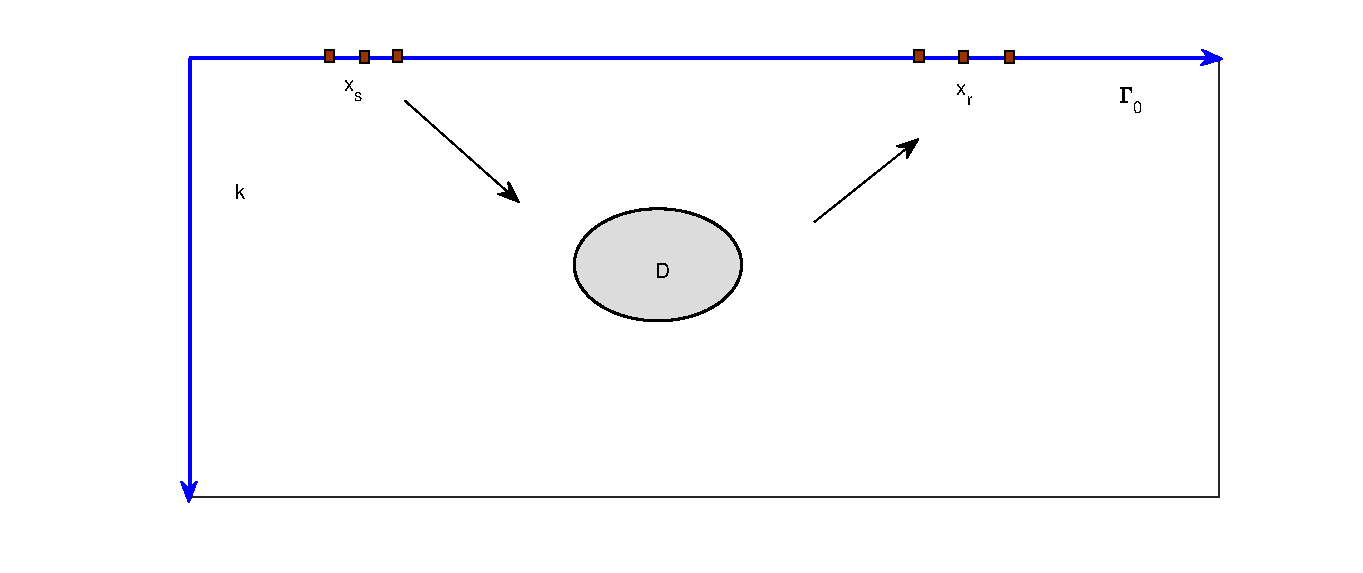
\includegraphics[width=\textwidth]{./Img/graphic/half_forward.eps}
	\caption{半空间弹性波障碍物散射模型} \label{figure_half}
\end{figure}
 令 $D\subset\R_+^2=\{(x_1,x_2)^T\in\R^2:x_2>0\}$ 是嵌入在半空间中的有界 Lipschitz 区域, 其中 $\nu$ 是边界 $\Ga_D$ 的单位外法向。 我们假设入射波是由位于半空间表面 $\Ga_0=\{(x_1,x_2)^T\in\R^2:x_2=0\}$ 上的 $x_s$ 的点源激发,且其激发的极化方向为 $q\in\R^2$。 假设半空间中的背景介质是弹性介质,且其表面满足自由边界条件 (Traction Free), 于是入射波即为半空间弹性波的 Neumann Green 函数 $\N(x,x_s)$ 。
假设接收点 $x_r\in \Ga_0$, 于是接受到的测量数据为 $u_q(x_r,x_s)=u^s_q(x_r,x_s)+\N(x_r,x_s)q, x_r\in\Ga_0$, 其中 $u_q^s(x,x_s)$ 是如下半空间弹性波方程的散射解。
\be
& &\Delta_e u_q^s(x,x_s)+ \rho\,\omega^2u_q^s(x,x_s)= 0 \ \ \ \ \mbox{in }\R_+^2\bks \bar{D},\label{p1}\\
& &u^s_q(x,x_s)=-\N(x,x_s)q \ \ \mbox{on} \ \Ga_D,\\
& & \sigma(u_q^s(x,x_s))e_2=0 \ \ \mbox{on} \ \Ga_0,\label{p2}
\ee
这里 
$e_i$ 是沿着 $x_i$, $i=1,2$ 轴的单位向量。

如何通过测量到的散射数据来确定散射体 $D$ 的位置、大小和形状就是本章将
要解决的问题。
\section{点扩散函数}
在这一节中, 我们将详细介绍半空间弹性波点扩散函数(point spread function)。 点扩散函数是一种针对半空间介质中点源的成像函数。 在文献 \cite{RTMhalf_aco} 中, Chen 等提出了半空间声波的点扩散函数, 我们这里将其推广到半空间弹性波的情形, 特别的, 此时的点扩散函数是一个 $2\times2$ 的矩阵。
假设在半空间的表面 $\Ga_0^d=\{(x_1,x_2)^T\in\Ga_0: x_1\in (-d,d)\}$ 上接受到的数据为 Neumann Green 函数 $\N(x,y)$, 即位于 $y$ 处的点源的数据, 这里 $d>0$ 称为孔径。 于是, 我们将有限孔径点扩散函数 $\J_d(x,y)$, $x,y\in\R^2_+$ 定义为将数据 $\N(x,y)\chi_{(-d,d)}$ 作为在 $\Ga_0$ 上的 Dirichlet 边界条件的反传波长, 这里 $\chi_{(-d,d)}$ 为区间 $\chi_{(-d,d)}$ 上的特征函数。 
更准确的来说, $\J_d(x,y)e_j, j=1,2,$ 是如下散射问题的解:
\ben
& &\De_e[\J_d(x,y)e_j]+\om^2[\J_d(x,y)e_j]=0\ \ \mbox{in }\R^2_+,\\
& &\J_d(x,y)e_j=[\overline{\N(x,y)}e_j]\chi_{(-d,d)}\ \ \mbox{on }\Ga_0.
\een
利用弹性波的积分表示公式, 我们有,对于任意 $z,y\in\R^2_+$ ,
\ben
[\J_d(z,y)]_{ij}&=&e_i\cdot[\J_d(z,y)e_j]\\
&=&\int_{\Ga_0^d}\T_D(x,z)e_i\cdot\overline{\N(x,y)}e_jds(x),\ \ i,j=1,2,
\een
利用矩阵表达, 可以简化为
\be\label{jd}
\J_d(z,y)=\int_{\Ga_0^d}\T_D(x,z)^T\overline{\N(x,y)}ds(x).
\ee

观察表达式 (\ref{jd}) 及定理\ref{es_NGT}, 定理 \ref{es_DGT}不难发现, 当 $d\to\infty$时, $\J_d(z,y)$ 收敛。 因此, 自然地, 我们就可以定义半空间弹性波点扩散函数 $\J(x,y)\in \C^{2\times 2}$, $x,y\in\R^2_+$, 即为
\be\label{j}
\J(z,y)=\int_{\Ga_0}\T_D(x,z)^T\overline{\N(x,y)}ds(x).
\ee
于是, 利用极限吸收原理, 我们有
\ben
\J(z,y)=\lim_{\ep\to 0^+}\int_{\Ga_0} \T_D^{\,\omega(1+\i\ep)}(x,z)^T\,
\overline{\N_{\om(1+\i\ep)}(x,y)}ds(x),
\een
这里 $\T_D^{\,\omega(1+\i\ep)}(x,z)q=\sigma(\D_{\om(1+\i\omega)}(x,z)q)e_2,\forall q\in\R^2$。
利用 Parserval 等式, Lemma \ref{cauchy_pv}, (\ref{d2}) and (\ref{d1}), 我们可以得到
\be
\J(z,y)&=&\frac{1}{2\pi}\sum_{\al,\beta=p,s}{\rm p.v.}\int_{\R}\frac{{\Ta}(\xi)^T \overline{\Nb(\xi)}}{\overline{\delta(\xi)}} e^{\i (\mu_\alpha z_2-\overline{\mu}_\beta y_2)+\i(y_1-z_1)\xi} d\xi \nn \\
& &-\frac\i 2\sum_{\al,\beta=p,s}\left[\frac{{\Ta}(\xi)^T \overline{\Nb(\xi)}}{\overline{\delta'(\xi)}} e^{\i (\mu_\alpha z_2-\overline{\mu}_\beta y_2)+\i(y_1-z_1)\xi}\right]^{k_R}_{-k_R}. \label{d3}
\ee
为了后文讨论方便, 我们把 $\J(z,y)$ 中的一部分定义为:
\be
\F(z,y)&=&\frac{1}{2\pi}\int^{k_p}_{-k_p} \  \frac{{\Tp}(\xi)^T \overline{\Np(\xi)}}{\overline{\delta(\xi)}} e^{\i \mu_p (z_2- y_2)+\i(y_1-z_1)\xi} d\xi\nn \\
&&+\frac{1}{2\pi}\int^{k_s}_{-k_s} \  \frac{{\Ts}(\xi)^T \overline{\Ns(\xi)}}{\overline{\delta(\xi)}} e^{\i \mu_s (z_2- y_2)+\i(y_1-z_1)\xi} d\xi. \label{d4}
\ee

在研究半空间弹性波点扩散函数之前, 我们先来定义成像函数的采样区域。 令 $\Omega$ 为成像函数的采样区域, 定义 $h=\dist(\Omega,\Gamma_0)$ 是 $\Omega$ 与 $\Gamma_0$ 的距离。 我们假设存在常数 $0<c_1<1,c_2>0$ 成立
\be\label{d0}
|x_1|\leq c_1 d , \ \ |x-y|\leq c_2 h ,\ \ \ \ \forall x,y \in \Omega.
\ee
\begin{remark}
	上述假设中, 第一个条件代表成像函数的采样区域不能太靠近孔径边缘, 第二个条件代表采样区域的尺寸相比于其与 $\Ga_0$的距离不能太大。第二个条件通常是合理的, 因为我们感兴趣的障碍物的尺寸大小要比入射波的波长小或是相当, 也就是 $k_s h\gg 1$。
\end{remark}

下面的引理不仅说明了 $\J(z,y)$ 是 $\J_d(z,y)$ 在 $d\to\infty$ 的极限, 而且还给出了 $\J_d(z,y)$ 与 $\J(z,y)$ 关于 $(h/d)$ 的误差估计。
\begin{lem} \label{error_jd}
	假设 $k_s h\geq 1$ 和 $d\gg h$ 。 对于任意 $z,y\in\Omega$ , 我们有
	\ben
	& &|\J(z,y)-\J_d(z,y)|+k_s^{-1}|\nabla_y(\J(z,y)-\J_d(z,y))| \\
	&\leq&\frac{C}{\mu} \left[\left(\frac{h}{d}\right)^{2}+(k_s h)^{1/2}e^{-k_s h\sqrt{\kappa_R^2-1}}\left(\frac{h}{d}\right)^{1/2}\right],
	\een
	这里常数 $C$ 只依赖于 $\kappa$ 。
\end{lem}
\debproof
我们利用定理 \ref{es_NGT} 和定理 \ref{es_DGT},作变量替换 $ t=x_1-z_1$,得到当 $k_s h\geq 1$ 和 $d\gg h$ 时有
\ben
& &\left| \int_{d}^{\infty} \left[\T_D(x,z)^T\overline{\N(x,y)}\right]_{x_2=0}dx_1
\right| \\
&\leq&
\frac{C}{\mu}\int_{d}^{\infty}\frac{k_s^{1/2} z_2}{|x-z|^{3/2}}\left(
\frac{k_s^{-1/2} y_2}{|x-y|^{3/2}}+e^{-\sqrt{k_R^2-k_s^2}y_2}\right) dx_1\\
&\leq&
\frac{C}{\mu}\int_{(1-c_1)d/h}^{\infty}\left(\frac{1}{(1+t^2)^{3/2}}+\frac{(k_s h)^{1/2}}{(1+t^2)^{3/4}} e^{-\sqrt{k_R^2-k_s^2}h}\right)  dt\\
&\leq&\frac{C}{\mu} \left[\left(\frac{h}{d}\right)^{2}+\frac{(k_s h)^{1/2}}{ e^{\sqrt{k_R^2-k_s^2}h}}\left(\frac{h}{d}\right)^{1/2}\right].
\een
上面的第二不等式我们使用了 (\ref{d0}) 的假定。 类似地, 我们也可以证明在 $(-\infty,-d)$ 上的不等式估计。 这就说明了 $\J(z,y)-\J_d(z,y)$ 的误差大小。 同样地, 针对 $\nabla_y(\J(z,y)-\J_d(z,y))$ 的估计也可以被证明。
\finproof

 有了以上引理, 现在我们可以只研究 $\J(z,y)$ 的性质, 然后通过引理 \ref{error_jd} 得到 $\J_d(z,y)$ 的性质。 由于我们只关心障碍物远离边界 $\Ga_0$ 时的情况, 即 $k_s h \gg 1$ , 所以, 针对点扩散函数 $\J(z,y)$, 我们希望将其分成两项, 其中第一项与 $k_s h$ 无关, 即主项; 第二项关于 $k_s h $ 是衰减的。
下面, 我们将说明当 $z,y\in\Om$时, $\F(z,y)$ 是 $\J_d(z,y)$ 的 $\F(z,y)$ 主项, 而且当 $|z-y|\to\infty$ 时, 它是衰减的。 特别地, 对于 $\F(z,y)$ 的虚部 $|\Im\F_{ii}(z,y)|, i=1,2$, 其在 $z=y$ 处存在峰值。

下面我们将用几个引理来说明 $\J_d(z,y)-\F(z,y)$ 关于 $k_s h$ 及 $h/d$ 的误差估计。 如下引理将说明式 (\ref{d3}) 中的第二项是随着 $k_s h$ 变大而指数衰减的。 

\begin{lem}\label{decay_1}
	存在只与 $\kappa$ 有关的常数 $C$, 当 $z,y\in\Om$ 时, 成立
	\ben
	\left|\sum_{\al,\beta=p,s}\left[\frac{{\Ta}(\xi)^T \overline{\Nb(\xi)}}{\overline{\delta'(\xi)}} e^{\i (\mu_\alpha z_2-\overline{\mu}_\beta y_2)+\i(y_1-z_1)\xi}\right]^{k_R}_{-k_R}\right|\le \frac C\mu e^{-\sqrt{k_R^2-k_s^2}h}.
	\een
\end{lem}
\debproof
观察式子 (\ref{d1}) , (\ref{d2}) ,我们发现, 对于 $\al=p,s$, 成立 $|\Ta(\pm k_R)|\le Ck_R^2/k_s^2\le C$, $|\Na(\pm k_R)|\le Ck_R^3$ 。利用引理 \ref{delta}, 该引理得证。
\finproof

\begin{lem}\label{lem:3.3}
	假设 $g(t)\in C^1(\R)\cap L^1(\R)$ 。存在只与 $\kappa$ 有关的常数 $C$,对于任意 $z,y\in\Om$ 成立
	\ben
	& & \left|{\rm p.v.}\int_{|\xi|>k_s}\frac{g(\xi)}{\delta(\xi)}d\xi\right| \\
	&\leq& Ck_s^{-4}\int_{|\xi|>k_s}|g(\xi)|d\xi+
	Ck_s^{-3}\max_{\xi\in(k_R-d_R,k_R+d_R)}(|g(\xi)|+k_s|g'(\xi)|).
	\een
	这里 $d_R =(k_R-k_s)/2$。
\end{lem}
\debproof
不失一般性,这里我们只针对在区间 $(k_s,\infty)$ 上的积分来证明该引理。 如引理 Lemma \ref{delta} 中一样, 我们有如下表示 $\de(\xi)=(\xi^2-k_R^2)\de_1(\xi)$ , 其中当 $\xi>k_s$ 时, $\de_1(\xi)\not=0$ 。 利用 Cauchy 主值的定义, 我们有
\be\label{l4}
\pv\int^\infty_{k_s}\frac{g(\xi)}{\delta(\xi)}d\xi&=&\int_{k_s}^{k_R-d_R}\frac{g(\xi)}{\delta(\xi)}d\xi+
\int^\infty_{k_R+d_R}\frac{g(\xi)}{\delta(\xi)}d\xi\nn\\
& &+\int^{k_R+d_R}_{k_R-d_R}\frac{g(\xi)((\xi+k_R)\de_1(\xi))^{-1}-g(k_R)(2k_R\de_1(k_R))^{-1}}{(\xi-k_R)}d\xi.
\ee
利用引理 \ref{delta}, 我们易得
\ben
\left|\int_{k_s}^{k_R-d_R}\frac{g(\xi)}{\delta(\xi)}d\xi+
\int^\infty_{k_R+d_R}\frac{g(\xi)}{\delta(\xi)}d\xi\right|\le Ck_s^{-4}\int^\infty_{k_s}|g(\xi)|d\xi.
\een
同样利用引理 \ref{delta} 中对 $\de(\xi),\de_1(\xi)$ 的估计及中值定理,我们可以得到
\ben
& &|\int^{k_R+d_R}_{k_R-d_R}\frac{g(\xi)((\xi+k_R)\de_1(\xi))^{-1}-g(k_R)(2k_R\de_1(k_R))^{-1}}{(\xi-k_R)}d\xi| \\
&\leq& 2d_R\max_{\xi\in(k_R-d_R,k_R+d_R)}(|\frac{g'(\xi)}{(\xi+k_R)\de_1(\xi)}|
\\
& &+|\frac{g(\xi)\delta_1(\xi)}{(\xi+k_R)\de_1(\xi))^2})|+|\frac{g(\xi)\delta_1'(\xi)}{(\xi+k_R)\de_1(\xi))^2}|)\\
&\leq&Ck_s^{-3}\max_{\xi\in(k_R-d_R,k_R+d_R)}(|g(\xi)|+k_s|g'(\xi)|)
\een
引理得证。
\finproof

下面的引理继续说明了 $\J(z,y)$ 中在区间 $|\xi|>k_s$ 上相应的积分是随 $k_s h$ 增大衰减的。
\begin{lem}\label{decay_2}
	令 $k_sh\ge 1$。 存在只与 $\kappa$ 有关的常数$C$, 对任意  $z,y\in\Om$ 成立
	\ben
	\left|\sum_{\al,\beta=p,s}{\rm p.v.}\int_{|\xi|>k_s}\frac{{\Ta}(\xi)^T \overline{\Nb(\xi)}}{\overline{\delta(\xi)}} e^{\i (\mu_\alpha z_2-\overline{\mu}_\beta y_2)+\i(y_1-z_1)\xi} d\xi\right|\le \frac C\mu(k_sh)^{-1}.
	\een
\end{lem}
\debproof
关于 $\al,\beta=p,s$, 我们定义 $g_{\al\beta}(\xi)=\Ta(\xi)^T\overline{\Nb(\xi)}e^{\i (\mu_\alpha z_2-\overline{\mu}_\beta y_2)+\i(y_1-z_1)\xi}$。于是利用引理 \ref{lem:3.3},我们可以易得
\ben
& &\left|\pv\int_{|\xi|>k_s}\frac{g_{\al\beta}(\xi)}{\overline{\de(\xi)}}d\xi\right| \\
&\le&\frac {C}{k_s^6\mu}\int^\infty_{k_s}|\xi|^5e^{-\sqrt{\xi^2-k_s^2}(y_2+z_2)}d\xi+\frac C\mu(k_sh) e^{-\sqrt{(k_R-d_R)^2-k_s^2}(y_2+z_2)}\\
&\le&\frac C\mu\int^\infty_1t^5e^{-\sqrt{t^2-1}k_s(y_2+z_2)}dt+\frac C\mu (k_sh) e^{-\sqrt{(k_R-d_R)^2-k_s^2}(y_2+z_2)}\\
&\le&\frac C\mu (k_sh)^{-1}+\frac C\mu (k_sh) e^{-\sqrt{(k_R-d_R)^2-k_s^2}(y_2+z_2)},
\een
这里我们使用了条件 $y_2,z_2 \geq h$ 和 $d_R=(k_R-k_s)/2\ge C_1k_s$, 其中常数 $C_1>0$ 只依赖于 $\kappa$。
又因为上面不等式的第二项是关于 $k_sh$ 指数衰减,则可以被 $(k_s h)^{-1}$ 控制。 引理得证。
\finproof
下面的引理将有助于我们分析在区间 $(-k_p,k_p)$ 上 , 当 $\al\neq\beta$时的积分。
\begin{lem}\label{cross_term}
	令 $\phi(t)=\sqrt{1-t^2}-\tau\sqrt{\kappa^2-t^2}+\nu t$, 这里 $\kappa\in (0,1), \tau\ge\tau_0>0, \nu\in\R$。
	存在仅依赖于 $\kappa, \tau_0$ 而与 $\nu$ 无关的常数 $C$ , 对于任意 $\lam\ge 1$ 以及 $f\in C[0,\kappa]$ 且其存在绝对连续的导函数, 成立:
	\ben
	& &
	\left|\int^\kappa_{-\kappa}f(t)e^{\i\lam\phi(t)}dt\right|+\left|\int^\kappa_{-\kappa}f(t)e^{-\i\lam\phi(t)}dt\right| \\
	&\leq& C\lambda^{-1/4}\left(|f(0)|+\int_{-\kappa}^{\kappa}|f'(t)|dt\right).
	\een
\end{lem}
\debproof
这里我们只要证明第一个在区间 $(0,\kappa)$ 上的积分的估计。 在区间 $(-\kappa,0)$ 上的积分的估计可以被类似证明,我们省略其证明细节。 通过简单的求导计算, 我们可以得到对于任意 $t\in (0,\kappa), m\ge 2$, 函数 $\phi(t)$ 的 $m$次导函数为 $\phi^{(m)}(t)=\tau\kappa^{-(m-1)}\psi_m(t/\kappa)-\psi_m(t)$, 其中
\ben
& &\psi_2(t)=(1-t^2)^{-3/2},\ \ \psi_3(t)=3t(1-t^2)^{-5/2},\ \  \\
& &\psi_4(t)=3(1+4t^2)(1-t^2)^{-7/2}.
\een
显然有, $\psi_m(t),m\ge 2$ 在区间 $(0,\kappa)$ 中是单调增函数。 

首先我们考虑当 $\tau\ge \kappa^2$ 时的情况。 这就意味着 $\tau\kappa^{-3}\ge\kappa^{-1}$ 而且有
\ben
\phi^{(4)}(t)\ge(\kappa^{-1}-1)\psi_4(t)\ge 3(\kappa^{-1}-1).
\een
利用 Van der Corput 引理 \ref{van},立即得到
\be\label{k2}
\left|\int^\kappa_{0}f(t)e^{\i\lam\phi(t)}dt\right|\leq C\lambda^{-1/4}\left(|f(0)|+\int_{-\kappa}^{\kappa}|f'(t)|dt\right).
\ee

接下去,我们考虑当 $\tau<\kappa^2$ 时的情况。 令 $\phi''(t)=0$, 可以得到
\ben
\tau\kappa^{-1}(1-(t/\kappa)^2)^{-3/2}=(1-t^2)^{-3/2}
\een 
易得 $\phi''(t)$ 在区间 $(0,\kappa)$ 上存在且只存在一个零点 $t=t_2$, 且有
\ben
t_2^2=\kappa^2-\frac{1-\kappa^2}{(\tau\kappa^2)^{-2/3}-1},
\een
观察 $\phi'''(t)$ , 我们可以得到, 当 $\kappa^3\le\tau<\kappa^2$ 时,在 $(0,\kappa)$ 上成立 $\phi'''(t)\ge 0$ ; 或是当 $\tau<\kappa^3$ 时, 有 $\phi'''(t)$ 在区间 $(0,\kappa)$ 上有且仅有一个零点 $t_3$, 且有
\ben
 t_3^2=\kappa^2-\frac{1-\kappa^2}{(\tau\kappa^2)^{-2/5}-1}.
\een
于是当 $\kappa^3\le\tau<\kappa^2$ 时, $\phi''(t)$在区间 $(0,\kappa)$ 为式单调增函数。 因此对于充分小的 $\de>0$,
\be\label{k3}
\hskip-1cm|\phi''(t)|\ge \min(|\phi''(t_2+\de)|,|\phi''(t_2-\de)|),\ \ \forall t\in (0,t_2-\de)\cup( t_2+\de,\kappa).
\ee
另一方面, 当$\tau<\kappa^3$ 时, 可以得到 $t_3<t_2$。而且成立当 $t\ge t_3$ 时有 $\phi'''(t)\ge 0$ 以及当 $t\le t_3$ 时有 $\phi'''(t)\le 0$ 。因此 $\phi''(t)$ 在区间 $(t_3,\kappa)$ 上单调递增而在 $(0, t_3)$ 上单调递减。 于是
\be\label{k4}
|\phi''(t)|\ge \min(|\phi''(t_2+\de)|,|\phi''(t_2-\de)|,|\phi''(0)|),\ \ \forall t\in (0,t_2-\de)\cup(t_2+\de,\kappa).
\ee

为了估计 $|\phi''(t_2\pm\de)|$ 的正下界, 我们观察到 $\tau\kappa^2<\kappa^4$。 因此, 我们得到 
\ben
t_2^2\ge\kappa^2-(1-\kappa^2)/(\kappa^{-8/3}-1).
\een
于是即得 $|\phi'''(t_2)|\ge c_0\tau\ge c_0\tau_0$ 其中常数 $c_0$ 仅依赖于 $\kappa$。
此外,对于任意 $t\in [t_2-\de,t_2+\de]$,有
\ben
|\phi'''(t)-\phi'''(t_2)|\le\max_{t\in [t_2-\de,t_2+\de]} |\phi''''(t)||t-t_2|\le c_1\de
\een
其中常数 $c_1$ 仅依赖于 $\kappa$。于是,如果取 $\de\le c_0\tau_0/(2C_1)$,对于$t\in[t_2-\de,t_2+\de]$, 就有 $|\phi'''(t)|\ge c_0\tau_0/2$。 

利用中值定理,我们可以得到 $|\phi''(t_2\pm\de)|\ge (c_0\tau_0/2)\de$。 观察到 $|\phi''(0)|=1-\tau\kappa^{-1}\ge 1-\kappa$, 从估计式 (\ref{k3})-(\ref{k4}) 我们可以得到对于充分小的 $\de>0$,
\be\label{k5}
|\phi''(t)|\ge (c_0\tau_0/2)\de,\ \ \forall t\in (0,t_2-\de)\cup( t_2+\de,\kappa).
\ee
现在,我们可以将积分分解成如下
\ben
& &\int^{\kappa}_0f(t)e^{\i\lam\phi(t)}dt\\
&=&\int^{t_2-\de}_0f(t)e^{\i\lam\phi(t)}dt+\int^{t_2+\de}_{t_2-\de}f(t)e^{\i\lam\phi(t)}dt+\int_{t_2+\de}^\kappa f(t)e^{\i\lam\phi(t)}dt\\
&:=&{\rm II}_1+{\rm II}_2+{\rm II}_3.
\een
利用不等式 (\ref{k5}) 及 Van der Corput 引理 \ref{van}, 我们有
\ben
|{\rm II}_1+{\rm II}_3| \le C(\lam\de)^{-1/2}\left(|f(0)|+\int^\kappa_0|f'(t)|dt\right).
\een
显然有 $|{\rm II}_2|\le 2\de\max_{t\in (0,\kappa)}|f(t)|$。我们取 $\de=\lam^{-1/3}$, 就可以得到
\ben
\left|\int^\kappa_{0}f(t)e^{\i\lam\phi(t)}dt\right|\leq C\lam^{-1/3}\left(|f(0)|+\int_{-\kappa}^{\kappa}|f'(t)|dt\right).
\een
联合 (\ref{k2}), 引理得证。
\finproof

下面的定理是本节的重要定理, 他说明了点扩散函数 $\J(z,y)$ 与其主项 $\F(z,y)$ 之间关于 $k_s h$ 的误差控制。
\begin{thm}\label{J_F_diff}
	令 $k_s h\ge 1$ 。存在只与 $\kappa$ 有关的常数 $C$, 对于任意 $z,y\in\Om$, 成立
	\ben
	|\J(z,y)-\F(z,y)|+k_s^{-1}|\na_y(\J(z,y)-\F(z,y))|\leq \frac{C}{\mu}(k_s h)^{-1/4}.
	\een
\end{thm}

\debproof
通过利用引理 \ref{decay_1}及引理 \ref{decay_2}, 观察 $\J(z,y),\F(z,y)$ 的定义 (\ref{d3})-(\ref{d4}), 我们只需要估计如下两项
\ben
& &\frac 1{2\pi}\sum_{\al,\beta=p,s}\int_{-k_s}^{k_s}\frac{{\Ta}(\xi)^T \overline{\Nb(\xi)}}{\overline{\delta(\xi)}} e^{\i (\mu_\alpha z_2-\overline{\mu}_\beta y_2)+\i(y_1-z_1)\xi} d\xi-\F(z,y)\\
\hskip-1cm&=&\frac {1}{2\pi}\sum_{\stackrel{\al,\beta=p,s}{_{(\al,\beta)\not= (s,s)}}}\int_{(-k_s,k_s)\backslash[-k_p,k_p]}\frac{{\Ta}(\xi)^T \overline{\Nb(\xi)}}{\overline{\delta(\xi)}} e^{\i (\mu_\alpha z_2-\overline{\mu}_\beta y_2)+\i(y_1-z_1)\xi} d\xi\\
\hskip-1cm&+&\frac 1{2\pi}\int_{-k_p}^{k_p}\left[\frac{\Tp(\xi)\overline{\Ns(\xi)}}{\overline{\de(\xi)}}e^{\i(\mu_py_2-\mu_s z_2)}+\frac{\Ts(\xi)\overline{\Np(\xi)}}{\overline{\de(\xi)}}e^{\i(\mu_sy_2-\mu_p z_2)}\right]e^{\i(y_1-z_1)\xi}d\xi\\
\hskip-1cm&:=&{\rm II}_1+{\rm II}_2.
\een
当 $k_p<|\xi|<k_s$ 时, 由引理 \ref{delta} 得, 我们知道有 $|\de(\xi)|\ge Ck_s^4$ 。 于是, 对于 $\al,\beta=p,s$, 我们有 $|\Ta(\xi)|\le C, |\Nb(\xi)|\le C\mu^{-1}k_s^2$。 于是, 我们马上可以得到如下不等式:
\ben
|{\rm II_1}|\le \frac{C}{k_s\mu}\int^{k_s}_{k_p}e^{-\sqrt{\xi^2-k_p^2}h}d\xi\le\frac C\mu (k_sh)^{-1}.
\een
而对于式子 ${\rm II}_2$ 我们将会使用引理 \ref{cross_term}。 通过简单的变量替换 $\xi=k_s t$, 我们可以把式 ${\rm II}_2$ 中的第一项转化成引理 \ref{cross_term} 中的形式, 即有
\ben
f(t)=k_s\frac{\Tp(k_st)\overline{\Ns(k_st)}}{\overline{\de(k_st)}},\ \ \ \lam=k_sz_2,\tau=\frac{y_2}{z_2},\nu=\frac{y_1-z_1}{z_2}.
\een
利用前面针对采样区域的尺寸的假设 (\ref{d0}), 直接利用引理 \ref{cross_term} 就可以得到,
\ben
\left|\int_{-k_p}^{k_p}\frac{\Tp(\xi)\overline{\Ns(\xi)}}{\overline{\de(\xi)}}e^{\i(\mu_py_2-\mu_s z_2)}d\xi\right|\le\frac{C}{\mu}(k_sh)^{-1/4}.
\een
而式子 ${\rm II}_2$ 中的第二项也可以被类似估计。 且 $|\na_y(\J(z,y)-\F(z,y))|$ 的估计也可以被类似证明, 这里不再赘述。 引理得证。
\finproof
\begin{figure}[htbp]
	\centering
	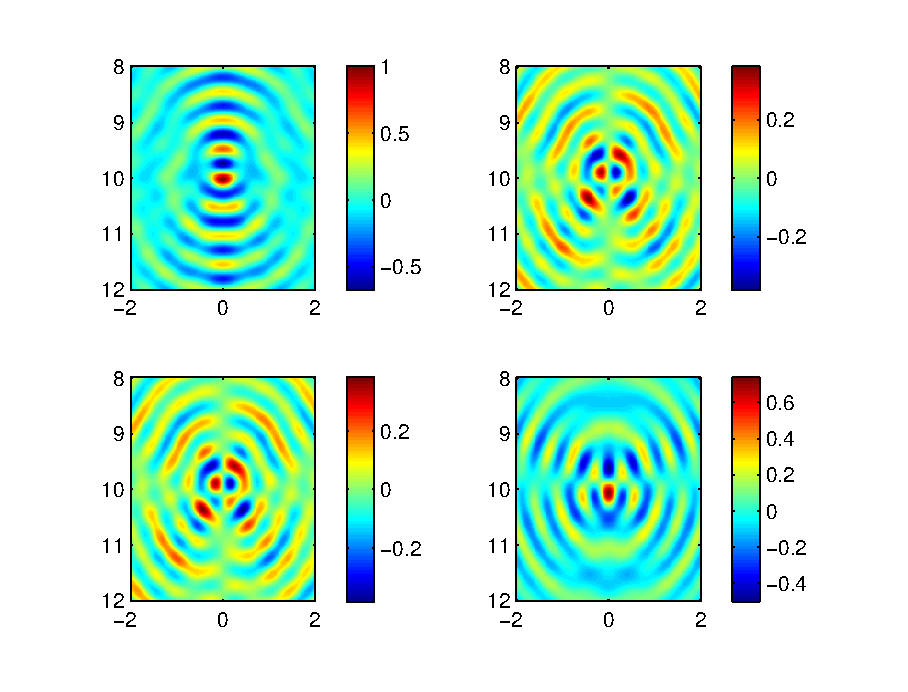
\includegraphics[width=\textwidth]{./Img/graphic/psf_om_2_lm_5_mu_25_im.eps}	
	\caption{$-Im(J_d(z,y))$ for $y=(0,8)^T$, $\omega=2\pi$, $d=100$}\label{figure_green}
\end{figure}
\begin{figure}[htbp]
	\centering
	\includegraphics[width=\textwidth]{./Img/graphic/green_om_2_lm_5_mu_25_im.eps}	
	\caption{$Im(G(z,y))$ for $y=(0,8)^T$, $\omega=2\pi$}\label{figure_psf}
\end{figure}

下面的引理告诉我们,点扩散函数 $\F(z,y)$ 的虚部与弹性波基本解 $\Im\G(z,y)$ 的虚部有相似的函数特性。于是, 利用定理 \ref{J_F_diff} 和引理 \ref{error_jd}, 当 $d\gg h$ 和 $k_s h\gg 1$, 我们可以认为 $\J_d(z,y)$ 的虚部也与弹性波基本解 $\Im\G(z,y)$ 的虚部有相似的函数特性, 见图 \ref{figure_psf} 和 图\ref{figure_green} 所展示。

\begin{remark}
	如图\ref{figure_psf} 和 图\ref{figure_green}中, 每幅图中4副子图, 其中子图的位置对应相应矩阵该位置的函数。其中, 每幅图的采样区域都为 $[-2,2]\times[8,12]$, 角频率 $\om=2\pi$, {Lam\'{e}} 常数 $\lambda=0.5$, $\mu=0.25$。 特别地, 每幅子图中, 颜色越深代表该处的值越大, 因此我们可以看到图\ref{figure_psf} 和 图\ref{figure_green}中对角线上的子图, 他们颜色的最深处正式图的中心位置, 即代表峰值在 $z=y$ 处。
\end{remark}
\begin{thm} \label{thm:3.2}
	对于任意 $z,y\in \R_+^2$, $\F(z,y)^T=\F(z,y)$。 当 $z=y$ 时,  $\Im [\F(z,y)]_{12} = \Im [\F(z,y)]_{21} =0$ 以及
	\be\label{d6}
	-\Im [\F(z,y)]_{ii}\geq \frac{1}{4(\lambda+2\mu)} \ , \ i =1 ,2.
	\ee
	当 $z\neq y$ 时,
	\be\label{d7}
	|\F(z,y)|&\le \frac{C}{\mu}\left(\frac 1{(k_s|z-y|)^{1/2}}+\frac 1{k_s|z-y|}\right),
	\ee
	这里的常数 $C$ 只依赖于 $\kappa$。
\end{thm}

\debproof
将式子 (\ref{d1}) 和式子 (\ref{d2}) 代入式子 (\ref{d4}), 我们可以得到
\be   
\F(z,y)&=&-\frac{1}{2\pi}\int_{-k_p}^{k_p} \frac{\i k_s^2\mu_s}{\mu\gamma(\xi)\delta(\xi)}
\Bigg(
\begin{array}{cc}
	\xi^2 & -\xi\mu_p \\
	-\xi\mu_p & \mu_p^2
\end{array}\Bigg)e^{\i\mu_p (z_2-y_2) +\i\xi(y_1-z_1)}d\xi \nn\\
\hskip-1.5cm& &-\frac{1}{2\pi}\int_{-k_p}^{k_p} \frac{\i k_s^2\mu_p}{\mu\gamma(\xi)\delta(\xi)}
\Bigg(
\begin{array}{cc}
	\mu_s^2 & \xi\mu_s \\
	\xi\mu_s & \xi^2
\end{array}		\Bigg)e^{\i\mu_s (z_2-y_2) +\i\xi(y_1-z_1)}d\xi \nn\\ 
\hskip-1.5cm& &
-\frac{1}{2\pi}\int_{(-k_s,k_s)\bks[-k_p,k_p]} \frac{\i(k_s^2-4\xi^2)\mu_p}{\mu\gamma(\xi)\overline{\delta(\xi)}}
\Bigg(
\begin{array}{cc}
	\mu_s^2 & \xi\mu_s \\
	\xi\mu_s & \xi^2
\end{array}		\Bigg)e^{\i\mu_s (z_2-y_2) +\i\xi(y_1-z_1)}d\xi \nn\\
\hskip-1.5cm&:=&{\rm III}_1+{\rm III}_2+{\rm III}_3. \label{d8}
\ee
由于 $\mu_p(\xi)$ 及 $\mu_s(\xi)$ 关于 $\xi$ 存在对称性, 所以我们易得当 $z=y$ 时, $\Im [\F(z,y)]_{12} = \Im [\F(z,y)]_{21} =0$。

现在我们来证明当 $i=j=1$ 时的不等式(\ref{d6}), 而其他情形时可以被类似证明, 这里将省略细节。 观察到, 当 $\xi\in (-k_p,k_p)$ 时,由引理 \ref{delta} 得 $\delta(\xi)\le k_s^4$ 及易得 $\mu_p\le\mu_s$。 于是当 $z=y$ 时:
\ben
& &-\Im ({\rm III}_1+{\rm III}_2)=\frac{1}{2\pi\mu}\int^{k_p}_{-k_p}\frac{k_s^2\mu_s}{\de(\xi)}d\xi\\
&\geq&\frac{1}{2\pi\mu}\int_{-k_p}^{k_p} \frac{\mu_p}{k_s^2}d\xi = \frac{1}{4(\lambda+2\mu)}.
\een
而当 $\xi\in(-k_s,k_s)\bks[-k_p,k_p]$时,成立 $\mu_p=\i\sqrt{\xi^2-k_p^2}$, 于是我们有
\ben
-{\rm III}_3=\frac{1}{2\pi\mu}\int_{(-k_s,k_s)\bks(-k_p,k_p)} \frac{-\mu_s^2\sqrt{\xi^2-k_p^2}(k_s^2-4\xi^2)}{(\xi^2+\i\mu_s\sqrt{\xi^2-k_p^2})(\varphi^2-\i4\xi^2\mu_s\sqrt{\xi^2-k_p^2})} d\xi.
\een
通过简单的直接计算, 我们有 \ben
\Im[(\xi^2+\i\mu_s\sqrt{\xi^2-k_p^2})(\varphi^2-\i4\xi^2\mu_s\sqrt{\xi^2-k_p^2})]=k_s^2\mu_s\sqrt{\xi^2-k_p^2}(k_s^2-4\xi^2).
\een
 通过分母有理化, 我们可以得到 $-\Im({\rm III}_3)\ge 0$。 因此, 当 $z=y$ 时, 我们有 $-\Im[\F(z,y)]_{11}\ge 1/[4(\lam+2\mu)]$ 。

当 $z\neq y$ 时, 我们可以有如下三角函数表示 $y-z=|y-z|(\cos\phi,\sin\phi)^T$ ,其中 $0\le\phi\le \pi$。 于是, 将此三角变量替换代入 ${\rm III}_1$, 我们可以得到
\ben
{\rm III}_1=\frac{1}{\mu}\int_{0}^{\pi} A(\theta,\kappa) e^{\i k_s |z-y| \cos(\theta-\phi)}d\theta,
\een
显然,简单的代入计算可以得到函数 $A(\theta,\kappa)$ 及其导函数 $\pa A(\theta,\kappa)/\pa\theta$ 在区间 $(0,\pi)$。 而且区间 $(0,\pi)$ 可以分割成若干个互补相交的子区间, 在每个子区间上成立 $|\cos(\theta-\phi)|\ge 1/\sqrt 2$ 或是 $|\sin(\theta-\phi)|\ge 1/\sqrt 2$ 以及 $-\sin(\theta-\phi)$ 在盖子区间上单调。 于是, 当$k_s|z-y|\ge 1$ 时,  Van der Corput 引理 \ref{van} , 我们易得
\ben
|{\rm III}_1|\le \frac C\mu\left(\frac 1{(k_s|z-y|)^{1/2}}+\frac 1{k_s|z-y|}\right).
\een
而当 $k_s|z-y|< 1$ 时,显然有 $|{\rm III}_1|\le C\mu^{-1}\le C\mu^{-1}(k_s|z-y|)^{-1}$。 而针对 ${\rm III}_2+{\rm III}_3$ 的估计可以类似地使用 Van der Corput 引理 \ref{van} 来证明。 引理得证。
\finproof

结合引理 \ref{error_jd}, 定理\ref{J_F_diff}, 定理\ref{thm:3.2} 及图\ref{figure_psf}, 我们发现点扩散函数 $J_d(z,y)$ 确实可以把位于 $y$ 的点源分辨出来, 即在 $z=y$ 处达到峰值, 在 $z$ 远离 $y$ 其值渐渐衰减。如文献 \cite{RTMhalf_aco} 中针对声波点扩散函数的表述, 我们也可以认为弹性波点扩展函数是对寻找弹性点源分辨率的度量函数。

为便于后文分析, 我们介绍如下在范数意义下的估计式。
\begin{lem}\label{lem:4.1}
	令 $k_s h\geq 1, d\gg h$, 存在只依赖于 $\kappa$ 却与 $k_s, h, d, d_D$ 无关的常数 $C$ , 对于任意 $z\in\Om$, $j=1,2$, 成立
	\ben
	& &\|\F(z,\cdot)e_j\|_{H^{1/2}(\Ga_D)}+\|\sigma(\F(z,\cdot)e_j)\nu\|_{H^{-1/2}(\Ga_D)}\le\frac C\mu(1+k_sd_D),\\
	& &\|\R_d(z,\cdot)e_j\|_{H^{1/2}(\Gamma_D)}+\|\sigma(\R_d(z,\cdot)e_j)\nu\|_{H^{-1/2}(\Gamma_D)} \le
	\frac{C}{\mu}(1+k_sd_D)\left[\left(\frac hd\right)^{2}+(k_sh)^{-1/4}\right],
	\een	
	其中 $\R_d(z,\cdot)=\J_d(z,\cdot)-\F(z,\cdot)$.
\end{lem}


\debproof
由 $\F(z,\cdot)$ 的定义 (\ref{d4}), 我们易得:
\ben
|F(z,y)|\leq \frac{C}{\mu}
\een 
于是, 上面第一估计式可有不等式 (\ref{q0}) 立即得到。 第二估计式可有不等式 (\ref{q0}), 由引理 \ref{error_jd} 和定理 \ref{J_F_diff} 立即得到。这里我们将不再赘述细节。 引理得证。
\finproof
\section{逆时偏移算法}
这一节, 我们将提出半空间弹性波散射问题的逆时偏移算法 (Reverse Time Migration, RTM)。 该逆时偏移算法是对文献 \cite{RTMhalf_aco} 中半空间声波散射问题的逆时偏移算法的一个推广。 我们的逆时偏移算法可以分成两步 \cite{zhang2009,Zhang2007}, 第一步为将在半空间表面的孔径 $\Ga_d$ 上接受到的 s-波与 p-波的混合全波数据取复共轭化, 然后反传到半空间中。 第二步,将反传后的数据和入射波数据在采样区域 $\Om$ 内进行互相关, 然后关于各个炮点进行叠加。特别地,类似与文献 \cite{RTMhalf_aco} , 这里的入射波是将点源放在 $\Ga_d$ 上, 然后作为 Dirichlet 边界条件后弹性波方程的解。而反传波是将接受到的数据共轭化后作为 Dirichlet 边界条件后弹性波方程的解。

\begin{alg}\label{alg_rtm}
	假设在 $\Ga_d$ 内均匀分布着 $N_s$ 个发射器, 位于 $x_s, \ s= 1,...,N_s$, 及分布着 $N_r$ 个接收器, 位于 $x_r, \ r=1,...,N_r$。 假设障碍物 $D\subset \Om$。 假设散射数据 $u_q^s(x_r,x_s)$ 为在 $x_r$ 处接受, 由位于 $x_s$ 处的点源沿着极化方向 $q=e_1, e_2$ 激发。
	
	$1^\circ$ 反传: 计算反传波 $v_q(x,x_s)$ 是如下半空间弹性波散射问题的解
	\ben
	& &\Delta_e v_q(x,x_s) + \omega^2 v_q(x,x_s) =0 \ \ \ \ \ \mbox{\rm in } \ \ \R^2_+, \\
	& &v_q(x,x_s)=\frac{|\Ga_0^d|}{N_r}\sum_{r=1}^{N_r}\overline{u_q^s(x_r,x_s)}\delta_{x_r}(x) \ \ \mbox{\rm on }  \ \ \Ga_d.
	\een
	
	$2^\circ$ 互相关: 对于任意 $q\in\R^2$,令入射波 $u^i_q$ 为如下半空间弹性波方程的解
	\ben
	& &\Delta_e u_q^i(x,x_s) + \omega^2 u_q^i(x,x_s) =0 \ \ \mbox{\rm in } \ \ \R^2_+,\ \ \\ & &u^i_q(x,x_s)=q\de_{x_s}(x)\ \ \mbox{on } \ \ \Ga_d.
	\een
	
	对于任意 $z\in\Om$, 计算成像函数:
	\be\label{cor1} 
	I_d(z)=\Im\sum_{q=e_1,e_2}\left\{\frac{|\Gamma_0^d|}{N_s}\sum^{N_s}_{s=1} u^i_q(z,x_s)\cdot v_q(z,x_s)\right\}. 
	\ee
\end{alg}
于是, 由 Green 表示公式可以得到:
\ben
& &u^i_q(x,x_s)=\T_D(x_s,x)^Tq, \\
& &v_q(x,x_s)\cdot e_j=\frac{|\Ga_0^d|}{N_r}\sum_{r=1}^{N_r}\T_D(x_r,x)e_j\cdot\overline{u_q^s(x_r,x_s)},
\een 
于是马上可以得到:
which yields
\be\label{cor}
I_d(z)=\Im\sum_{q=e_1,e_2}\left\{\frac{|\Gamma_0^d|^2}{N_sN_r}\sum^{N_s}_{s=1}\sum^{N_r}_{r=1}
[\T_D(x_s,z)^Tq]\cdot[\T_D(x_r,z)^T\overline{u^s_q(x_r,x_s)}]\right\}.
\ee

上面的成像函数是离散形式的, 可以直接用于数值计算。 为了便于后面的理论分析, 我们令 $N_s,N_r\to\infty$, 于是离散形式的成像函数 (\ref{cor1}) 可以看成是采用数值积分对如下连续形式的成像函数的一种积分逼近:
\be
\hat{I}_d(z)=\Im\sum_{q=e_1,e_2}\int_{\Gamma_0^d}\int_{\Gamma_0^d}\,
[\T_D(x_s,z)^Tq]\cdot[\T_D(x_r,z)^T\overline{u^s_q(x_r,x_s)}]\,ds(x_r)ds(x_s).\label{cor2}
\ee


下面我们将障碍物的成像函数 $\hat I_d(z)$ 与前文中的点扩散函数 $\J_d(z,y)$ 联系起来。 有了前文中对 $\J_d(z,y)$ 相关分析结论,我们可以由此来分析半空间反弹性波散射问题的逆时偏移方法的分辨率。下面的定理, 告诉我们当采样点 $z$ 远离障碍物边界的时候, 成像函数在改点的值是非常小的。这种现象反映在后面的数值实验中, 就是在原理边界的时候, 在该处的颜色会非常浅。下面的定理是当障碍物边界为 $Dirichlet$ 边界时的成像函数分辨率分析。 其它边界条件的相关结论可以被类似证明, 我们会不加证明地罗列在后文。
\begin{thm}\label{thm:4.3}
	对于任意 $z\in\Omega$, 令 $\U(z,x)\in\C^{2\times2}$ 且 $\U(z,x)e_j$, $j=1,2$, 是如下弹性波方程的散射解:
	\ben
	& &\Delta_e [\U(z,x)e_j]+ \omega^2[\U(z,x)e_j]= 0 \ \  \ \ x\in\R^2\bks \bar{D},  \\
	& &
	\U(z,x)e_j= -\overline{\F(z,x)}e_j \ \  \ \ x\in\Ga_D.  
	\een
	于是, 成像函数 $\hat{I}_d(z)$ 有如下表达:
	\be
	\hat{I}_d(z)=\Im\sum_{j=1}^2\int_{\Gamma_D}[\sigma(\U(z,x)e_j+\overline{\F(z,x)}e_j)\nu]\cdot [\overline{\F(z,x)}e_j]ds(x)+R_d(z),\label{id}
	\ee
	这里 
	\ben
	|R_d(z)|\leq C\mu^{-2}(1+\|T_1\|)(1+\|T_2\|)(1+k_s d_D)^3\left[\left(\frac hd\right)^{2}+(k_sh)^{-1/4}\right],
	\een
	其中常数 $C$ 仅依赖与 $\kappa$ 而与 $k_s,k_p, h, d, d_D$ 无关。
\end{thm}
\debproof
观察算法中的 (\ref{cor2}) 我们可以得到:
\be\label{g5}
\hat I_d(z)=\Im\sum_{q=e_1,e_2}\int_{\Ga_0^d}[\T_D(x_s,z)^Tq]\cdot\hat v_q(z,x_s)ds(x_s),
\ee
其中 $j=1,2$,
\ben
\hat v_q(z,x_s)\cdot e_j=\int_{\Ga_0^d}\T_D(x_r,z)e_j\cdot\overline{u^s_q(x_r,x_s)}ds(x_r).
\een
利用 (\ref{g2}) 我们得到 
\ben
u^s_q(x_r,x_s)\cdot e_i=\GG(u^s_q(\cdot,x_s),\N(\cdot,x_r)e_i), i=1,2,
\een
 于是有
\ben
\hat v_q(z,x_s)\cdot e_j&=&\int_{\Ga_0^d}\T_D(x_r,z)e_j\cdot\overline{[u^s_q(x_r,x_s)\cdot e_1,u^s_q(x_r,x_s)\cdot e_2]^T}ds(x_r)\\
&=&\GG(\overline{u^s_q(\cdot,x_s)},\left[\int_{\Ga_0^d}\sum^2_{i=1}[\T_D(x_r,z)]_{ij}\overline{\N(\cdot,x_r)}e_ids(x_r)\right]\,).
\een
利用 Neumann Green 函数的空间互易性 
\ben
\N(x,x_r)=\N(x_r,x)^T,
\een
 以及点扩展函数 $\J_d(\cdot,\cdot)$ 的定义 (\ref{jd}), 我们有
\be\nn
& &\int_{\Ga_0^d}\sum^2_{i=1}[\T_D(x_r,z)]_{ij}\overline{\N(x,x_r)}e_ids(x_r)\\ \nn
&=&\int_{\Ga_0^d}\sum^2_{i=1}[\T_D(x_r,z)]_{ij}\overline{\N(x_r,x))^Te_i}ds(x_r)\\ \nn
&=&\int_{\Ga_0^d}(\T_D(x_r,z)e_j)^T\overline{\N(x_r,x)^T)}ds(x_r) \\  \nn
&=&\J_d(z,x)^Te_j. v \label{g6}
\ee
进一步可以推出
 \ben
 \hat v_q(z,x_s)e_j=\GG(\overline{u^s_q(\cdot,x_s)},\J_d(z,\cdot)^Te_j).
 \een
  将上式代入 (\ref{g5}) 中, 我们可以得到
\be\nn
\hat I_d(z)&=&\Im\sum_{j=1}\sum_{q=e_1,e_2}\int_{\Ga_0^d}[\T_D(x_s,z)^Tq\cdot e_j][\hat v_q(z,x_s)\cdot e_j]ds(x_s)
\\  \nn
&=&\Im\sum_{j=1}^2\GG(\sum_{k=1}^2[\T_D(x_s,z)^Te_k\cdot e_j]\overline{u^s_{e_k}(x,x_s)},\J_d(z,\cdot)^Te_j)
\\ 
\label{g3}
&=&\Im\sum_{j=1}^2\GG(\W(z,\cdot)e_j,\J_d(z,\cdot)^Te_j),
\ee
这里 $\W(z,x)\in \C^{2\times 2}$ 是一个 $2\times2$ 的矩阵, 定义为
\ben
\W(z,x)e_j=\int_{\Ga_0^d}\sum^2_{k=1}[\T_D(x_s,z)]_{kj}\overline{u^s_{e_k}(x,x_s)}ds(x_s),\ \ j=1,2.
\een
注意到 $\overline{\W(z,x)}e_j$ 可以看成是 $u^s_{e_k}(x,x_s)$ 加权叠加, 于是它满足如下方程:
\be\label{g7}
& &\De_e[\overline{\W(z,x)}e_j]+\om^2[\overline{\W(z,x)}e_j]=0\ \ \mbox{in } \ \R^2_+\bks\bar D,\ \ \ \\
& & \sigma(\overline{\W(z,x)}e_j)e_2=0\ \ \mbox{on } \ \Ga_0.
\ee
由于在边界 $\Gamma_D$, $u^s_{e_k}(x,x_s)$ 满足 Dirichlet 边界条件,即 $u^s_{e_k}(x,x_s)=-\N(x,x_s)e_k$。 于是利用式 (\ref{g6}) 我们得到
\be\nn
& &\overline{\W(z,x)}e_j\\ \nn
&=&-\int_{\Ga_0^d}\sum^2_{k=1}[\overline{\T_D(x_s,z)}]_{kj}\N(x,x_s)e_kds(x_s) \\
&=&-\overline{\J_d(z,x)}^Te_j.\label{g8}
\ee
现在我们定义矩阵 $\W_d(z,x)\in \C^{2\times 2}$ , 其中向量  $\W_d(z,x)e_j$, $j=1,2$ , 是如下半空间弹性波方程的散射解:
\be
& & \Delta_e [\W_d(z,x)e_j]+ \omega^2 [\W_d(z,x)e_j]= 0 \ \ \ \ \mbox{in }\R^2_+\bks \bar{D},\label{g9}\\
& &\W_d(z,x)e_j= -\overline{\F(z,x)}e_j \ \ \mbox{on } \ \ \Ga_D,\ \ \ \  \\
& &\sigma(\W_d(z,x)e_j)e_2=0 \ \ \ \ \ \ \ \mbox{on }  \ \ \ \Ga_0 \label{g10}
\ee
利用 (\ref{g3}) 我们可以推出:
\be
\hat I_d(z)&=&\Im\sum^2_{j=1}\GG(\W(z,\cdot)e_j,J_d(z,\cdot)^Te_j-\F(z,\cdot)e_j)\nn\\
& &+\Im\sum^2_{j=1}\GG(\W(z,\cdot)e_j-\overline{\W_d(z,\cdot)}e_j,\F(z,\cdot)e_j)\nn\\
& &+\Im\sum^2_{j=1}\GG(\overline{\W_d(z,\cdot)}e_j-\overline{\U(z,\cdot)}e_j,\F(z,\cdot)e_j)\nn\\
& &+\Im\sum^2_{j=1}\GG(\overline{\U(z,\cdot)}e_j,\F(z,\cdot)e_j) \nn \\
&:=&{\rm VI}_1+{\rm VI}_2+{\rm VI}_3+{\rm VI}_4.\label{g11}
\ee
观察 $\F(z,y)$ 的定义 ($\ref{d4}$), 易得 $\F(z,y)^T=\F(z,y)$。 利用引理 \ref{lem:4.1}, 
\ben
& &\|\J_d(z,\cdot)e_j\|_{H^{1/2}(\Ga_D)}+\|\sigma(\J_d(z,\cdot)e_j)\nu\|_{H^{-1/2}(\Ga_D)}\\ &\le&
\|\F(z,\cdot)e_j\|_{H^{1/2}(\Ga_D)}+\|\sigma(\F(z,\cdot)e_j)\nu\|_{H^{-1/2}(\Ga_D)}\\
& &+\|\R_d(z,\cdot)e_j\|_{H^{1/2}(\Ga_D)}+\|\sigma(\R_d(z,\cdot)e_j)\nu\|_{H^{-1/2}(\Ga_D)}\\
&\le&\frac C\mu (1+k_sd_D).
\een
这就意味着,通过 (\ref{g7})-(\ref{g8}) 以及引理 \ref{lem:4.1}, 可以得到:
\ben
|{\rm VI}_1|&\le&\sum_{j=1}^2\Big(\|\W(z,\cdot)e_j\|_{H^{1/2}(\Ga_D)}\|\sigma(\J_d(z,\cdot)^Te_j-\F(z,\cdot)e_j)e_2\|_{H^{-1/2}(\Ga_D)}\\
& &+\|\sigma(\W(z,\cdot)e_j)e_2\|_{H^{-1/2}(\Ga_D)}\|\J_d(z,\cdot)^Te_j-\F(z,\cdot)e_j\|_{H^{1/2}(\Ga_D)}\Big)\\
&\le&\frac C{\mu^2}(1+\|T_1\|)(1+k_sd_D)^2\left[\left(\frac hd\right)^{2}+(k_sh)^{-1/4}\right].
\een
类似地, 通过 (\ref{g7})-(\ref{g8}) 和 (\ref{g9})-(\ref{g10}), 及引理 \ref{lem:4.1} , 可以得到:
\ben
|{\rm VI}_2|\le\frac C{\mu^2}(1+\|T_1\|)(1+k_sd_D)^2\left[\left(\frac hd\right)^{2}+(k_sh)^{-1/4}\right].
\een
对于第三项 ${\rm VI}_3$, 我们可以针对 $\W_d(z,x)$ 和 $\U(z,y)$, 使用定理 \ref{thm:4.2} 和引理 {\ref{lem:4.1}, 可以得到:
	\ben
	|{\rm VI}_3|\le\frac C{\mu^2}(1+\|T_1\|)(1+\|T_2\|)(1+k_sd_D)^3(k_sh)^{-1/2}.
	\een
	最后, 由定义有, 当$z\in\Ga_D$ 时 $\U(z,x)e_j=-\overline{\F(z,x)}e_j$  $\Ga_D$。 于是,可以推出
	\ben
	{\rm IV}_4&=&\Im\sum^2_{j=1}\int_{\Ga_D}(\overline{\U(z,x)}e_j\cdot\sigma(\F(z,x)e_j)\nu-\sigma(\overline{\U(z,x)}e_j)\nu\cdot\F(z,x)e_j)ds(x)\\
	\hskip-1.5cm&=&-\Im\sum^2_{j=1}\int_{\Ga_D}\sigma(\overline{\U(z,x)}e_j+\F(z,x)e_j)\nu\cdot\F(z,x)e_jds(x)\\
	\hskip-1.5cm&=&\Im\sum^2_{j=1}\int_{\Ga_D}\sigma(\U(z,x)e_j+\overline{\F(z,x)}e_j)\nu\cdot\overline{\F(z,x)}e_jds(x).
	\een
	综上所述, 利用式子 (\ref{g11}), 引理得证。
	\finproof


由于本文中关心的障碍物都为扩展障碍物(Extended Obstacles),即为 $k_s d_D\approx 1$。由于 $k_s=2\pi/\lambda_s$, 这里 $\lambda_s$ 为 s-波的波长, 于是意味着障碍物的尺寸与入射波的s-波的波长相当。然后,通过定理 \ref{thm:4.3}, 我可以看到, 当障碍物 $D$ 远离半空间表面 $\Ga_0$ 时, 即 $k_s h \gg 1$, 且孔径较大时,即 $d\gg h$, 我们可以认为 $\R_d(z)$ 是非常小的。于是, 我们在这种情况下可以把式 (\ref{id}) 右端第一项看作是该成像函数的 $\hat I_d(z)$ 的主项
\ben
\hat{I}_d(z)&\approx&\Im\sum_{j=1}^2\int_{\Gamma_D}[\sigma(\U(z,x)e_j+\overline{\F(z,x)}e_j)\nu]\cdot [\overline{\F(z,x)}e_j]ds(x) \\
&:=&\hat{I}_F(z)
\een 

观察 $\F(z,x)$ 的表达式 (\ref{d8}), 对于任意 $z\in\Om$,存在标量函数 $A_j(\xi), B_j(\xi)$, $j=1,2$,可以将 $\F(z,x)$ 表示成
\ben\nn
\F(z,x)e_j&=&\int_{-k_p}^{k_p}A_j(\xi)\left(\begin{array}{c}
	\hskip-6pt-\xi \hskip-6pt \\
	\hskip-6pt \mu_p \hskip-6pt
\end{array}\right)e^{\i(z-x)\cdot(-\xi,\mu_p)^T}d\xi\\ \nn
& &+\int_{-k_s}^{k_s}B_j(\xi)\left(\begin{array}{c}
	\hskip-6pt\mu_s \hskip-6pt\\
	\hskip-6pt\xi \hskip-6pt
\end{array}\right)e^{\i(z-x)\cdot(-\xi,\mu_s)^T}d\xi\\ \nn
&=&\int^\pi_0\tilde A_j(\theta)\tau(\theta)e^{\i k_p(z-x)\cdot\tau(\theta)}d\theta \\  \label{F_theta}
& &+\int^\pi_0\tilde B_j(\theta)\tau(\theta)^\perp e^{\i k_s(z-x)\cdot\tau(\theta)}d\theta,
\een
其中第二个等式使用了变量替换 $\xi=\cos\theta$, 且有
\ben
 & &\tilde A_j(\theta)=k_pA_j(k_p\cos\theta)\sin\theta, \\
 & &  \tilde B_j(\theta)=k_sB_j(k_s\cos\theta)\sin\theta, \\ 
 & &\tau(\theta)=(-\cos\theta,\sin\theta)^T, \ \\ 
 & &\tau(\theta)^\perp=(\sin\theta,\cos\theta)^T.
\een

于是 $\overline{\F(z,x)}e_j$ 可以看成是弹性波 $p$ 平面波加权叠加与 $s$ 平面波的加权叠加之和, 显然对于固定的 $z$, $\overline{\F(z,x)}e_j$ 关于变量 $x$ 满足弹性波方程。 因此, 由 $\U(z,x)e_j$ 的定义, 自然地可以把它看成是以 $\overline{\F(z,x)}e_j$ 为入射波且满住 Dirichlet 边界条件的弹性波散射解。 通过定理 \ref{thm:3.2} , 我们知道 $\overline{\F(z,x)}$ 随着 $|x-z|$ 增大而逐渐衰减。于是易知, 当$x\in \Ga_D$ 时,$\sigma(\U(z,x)e_j+\overline{\F(z,x)}e_j)\nu$ 也随着 $|x-z|$ 增大而逐渐衰减。 因此, 当点 $z$ 远离障碍物边界 $\Ga_D$ 时, $\hat{I}_F(z)$ 变得非常小。 于是, 当 $k_s h \gg 1$ , $d\gg h$ 以及 $z$ 远离障碍物边界 $\Ga_D$ 时, $\hat{I}_d(z)$ 变得非常小, 即此时在 $z$ 点无法成像。

为了分析当 $z$ 靠近障碍物边界时成像函数主项$\hat{I}_F(z)$ 的函数性质, 我们将提出平面入射波在障碍物边界处的散射系数。 类似与声波散射系数, 我们将给弹性波散射系数如下定义。

\begin{definition}\label{scarr_con}
	对于任意单位向量 $\tau\in \R^2$, 令 $u^i_p =\tau e^{\i k_p x\cdot \tau}$ ,  $u^i_s= \tau^\perp e^{\i k_s x\cdot \tau}$ 分别是 $p$ 平面入射波和 $s$ 平面入射波。   令 $u^s_\alpha (x) := u^s_\alpha(x;\tau), \al=p,s$ 为相应的弹性波散射解:
	\be\label{sc1}
	& &\De_e u^s_\alpha + \om^2u^s_\alpha = 0\ \ \mbox{in }   \ \ \R^2\bks\bar{D}, \ \ \ \  \\
	& & u^s_\alpha =-u^i_\alpha \ \ \mbox{on }  \ \ \Ga_D.
	\ee
	于是相应的散射系数 $R_\al(x;\tau)$, $x\in\Ga_D$ 满足如下关系
	\ben
	\sigma(u^s_\alpha(x)+u^i_\alpha(x))\nu(x)= \i k_\alpha R_\alpha(x;\tau)e^{\i k_\alpha x\cdot \tau}  \ \ \ \mbox{on } \ \ \  \Ga_D.
	\een
	其中对于 $\tau=(\tau_1,\tau_2)^T\in\R^2$,, 有$\tau^\perp=(\tau_2,-\tau_1)^T$。
\end{definition}
\begin{remark}
	由全空间弹性波散射问题的唯一性和存在性 \cite{cxz2016,ku63}, 可以认为散射系数的定义是合理的。 类似地, 我们可以针对其它障碍物边界条件, 如 Neumann 边界条件, Robbins 边界条件 等, 也可以定义相应的散射系数。 特别地, 上面定义的散射系数是对文献\cite{RTMhalf_aco} 中的声波散射系数的推广。
\end{remark}

事实上, 由弹性波散射系数的定义可知, 当得知入射波与散射系数时,我们就可以得到在障碍物处表面的弹性总场的法向应力。 于是下面我们将来讨论, 如何去逼近弹性波的散射系数。自然地, 我们先来讨论最简单的情形, 当障碍物为一平面时的散射系数。特别地,先假设平面为 $x_1$ 轴。

\subsection{反射面为$x_1$轴}

我们考虑入射波为 $p$ 平面波 $\hat u_p$ (或是 $s$-wave $\hat u_s$) ,其中入射方向为 $\hat d_0=(\sin t_0, \cos t_0)^T, t_0\in (0,2\pi)$。 反射平面为 $\Gamma := \{x \in \R^2 :x _2 = 0\}$, 于是法向为 $\hat\nu=(0,1)^T$。


\subsubsection{$p$-波情形}
我们定义入射波 $p$ 平面波 \cite[p172]{achenbach1980} 如下:
\ben
& &\hat u_p=A_0(\sin t_0,\cos t_0)^Te^{\i k_p(x_1\sin t_0+x_2 \cos t_0)}.
\een
于是, 反射 $p$ 波可以被表示成:
\ben
& &\hat u_{p,p}=A_1(\sin t_1,-\cos t_1)^Te^{\i k_p(x_1\sin t_1-x_2 \cos t_1)}.
\een
 反射 $s$ 波可以被表示成:
\ben
& &\hat u_{p,s}=A_2(-\cos t_2,-\sin t_2)^Te^{\i k_s(x_1\sin t_2-x_2 \cos t_2)}.
\een
由于在反射面 $\Ga$ 上满足 Dirichlet 边界条件, 于是马上可以得到:
\ben
\hat u_p(x_1,0)+\hat u_{p,p}(x_1,0)+\hat u_{p,s}(x_1,0)=0,\ \ \forall x_1\in\R.
\een
通过简单的计算可以得到:
\ben
& & t_1=t_0, \ \ \frac{\sin t_2}{\sin t_0}=\frac{k_p}{k_s}:=\kappa, \\
& & \frac{A_1}{A_0}=\frac{\cos(t_0+t_2)}{\cos(t_0-t_2)}, \ \ \ \  \\
& & \frac{A_2}{A_0}=\frac{\sin 2t_0}{\cos(t_0-t_2)}.
\een 
于是, 易知当入射角 $t_0\neq0$ 时, 入射波为 p 平面波时, 不仅会引发 p 反射波, 而且有 s 反射波。
特别地, 若我们可以将总场表示成如下向量形式:
\be\label{a1}
\hat u^{\rm total}_p=A_0\hat d_0e^{\i k_px\cdot\hat d_0}+A_1\hat d_1e^{\i k_px\cdot\hat d_1}+A_2\hat d_2^\perp e^{\i k_s x\cdot\hat d_2},
\ee
这里对于任意 $\tau=(\tau_1,\tau_2)^T\in\R^2$, 有 $\tau^\perp=(\tau_2,-\tau_1)^T$, 且其中有:
\be
& &\hat d_1=\hat d_0-2(\hat d_0\cdot\hat\nu)\hat\nu, \\
& &\hat d_2=\kappa\hat d_0-\left[\kappa(\hat d_0\cdot\hat\nu)+{\rm sgn}(\hat d_0\cdot\hat\nu)\sqrt{1-\kappa^2(\hat d_0\cdot\hat\nu^\perp)^2}\,\right]\hat\nu,\\
& &\frac{A_1}{A_0}=\frac{-\hat d_0\cdot\hat d_2}{\hat d_1\cdot\hat d_2}, \ \  \ \ \\
& &\frac{A_2}{A_0}=\frac{2(\hat d_0\cdot\hat\nu)(\hat d_0\cdot\hat\nu^\perp)}{\hat d_1\cdot\hat d_2}.\label{a2}
\ee

\subsubsection{$s$-波情形}
类似地, 我们可以定义 $s$ 平面波如下
\ben
& &\hat u_s=A_0(\cos t_0,-\sin t_0)^Te^{\i k_s(x_1\sin t_0+x_2 \cos t_0)}.
\een
于是, 反射 $p$ 波可以被表示成:
\ben
& &\hat u_{s,p}=A_1(\sin t_1,-\cos t_1)^Te^{\i k_p(x_1\sin t_1-x_2 \cos t_1)}.
\een
反射 $s$ 波可以被表示成:
\ben
& &\hat u_{s,s}=A_2(-\cos t_2,-\sin t_2)^Te^{\i k_s(x_1\sin t_2-x_2 \cos t_2)}.
\een
同理, 由于在反射面 $\Ga$ 上满足 Dirichlet 边界条件, 于是马上可以得到:
\ben
\hat u_s(x_1,0)+\hat u_{s,p}(x_1,0)+\hat u_{s,s}(x_1,0)=0,\ \ \forall x_1\in\R.
\een
通过简单的计算可以得到:
\ben
& &t_2=t_0,\ \ \frac{\sin t_1}{\sin t_0}=\frac{k_s}{k_p}=\kappa_1,\\
& & \frac{A_1}{A_0}=\frac{-\sin 2t_0}{\cos(t_0-t_1)}, \ \ \\
& &\frac{A_2}{A_0}=\frac{\cos(t_0+t_1)}{\cos(t_0-t_1)}
\een
于是, 易知当入射角 $t_0\neq0$ 时, 入射波为 s 平面波时, 不仅会引发 s 反射波, 而且有 p 反射波。
特别地, 若我们可以将总场表示成如下向量形式:
\be\label{b1}
\hat u^{\rm total}_s=A_0\hat d_0^\perp e^{\i k_sx\cdot\hat d_0}+A_1\hat d_1e^{\i k_px\cdot\hat d_1}+A_2\hat d_2^\perp e^{\i k_s x\cdot\hat d_2},
\ee
其中
\be
& &\hat d_1=\kappa_1\hat d_0-\left[\kappa_1(\hat d_0\cdot\hat\nu)+{\rm sgn}(\hat d_0\cdot\hat\nu)\sqrt{1-\kappa_1^2(\hat d_0\cdot\hat\nu^\perp)^2}\,\right]\hat\nu,  \\
& &\hat d_2=\hat d_0-2(\hat d_0\cdot\hat\nu)\hat\nu,\\
& &\label{b2} \frac{A_1}{A_0}=\frac{-2(\hat d_0\cdot\hat\nu)(\hat d_0\cdot\hat\nu^\perp)}{\hat d_1\cdot\hat d_2}, \ \  \  \ \\
& &\frac{A_2}{A_0}=\frac{-\hat d_0\cdot\hat d_1}{\hat d_1\cdot\hat d_2}
\ee

\subsection{反射面为任意平面}

我们考虑入射波为 $p$ 平面波 $u_p$ (或是 $s$-wave  $u_s$) ,其中入射方向为 $ d_0=(\sin t_0, \cos t_0)^T, t_0\in (0,2\pi)$。 反射平面为 $\Gamma := \{x \in \R^2 : x \cdot \nu = 0\}$ , 该反射面穿过原点, 且其法向量为 $\nu=(\sin\phi,\cos\phi)^T,\phi\in (0,2\pi)$。  我们将其总场表示为;
\be
u_p^{\rm total}=A_0d_0 e^{\i k_p x\cdot d_0}+A_1 d_1 e^{\i k_p x\cdot d_1}+A _2d_2^\perp e^{\i k_s x\cdot d_2},\\
u_s^{\rm total}=A_0d_0^\perp e^{\i k_s x\cdot d_0}+A_1 d_1 e^{\i k_p x\cdot d_1}+A_2 d_2^\perp e^{\i k_s x\cdot d_2},
\ee
这里 $i=0,1,2$, $d_i$ 是单位向量, $A_i$ 是相应的振幅。由于在反射面$\Ga$ 上满足 Dirichlet 边界条件, 意味着有 $u_p^{\rm total}=0, u_s^{\rm total}=0$ , $x\in\Gamma$。 为了将任意平面与 $x_1$ 轴联系起来, 我们令  
$\hat x= S x$, 这里 $S\in\R^{2\times 2}$ 是旋转角度为 $\phi$ 的旋转矩阵, 即为
\ben
S= \left( \begin{array}{ll}
	\cos\phi& -\sin\phi \\
	\sin\phi & \cos\phi
\end{array}\right).
\een
定义 $\hat\nu=S\nu$。下面的定理告诉我们, 当 $u(x)$ 在坐标 $x$ 下满足弹性波方程时, 则$u(x)$ 在旋转后得到的 $S u(x)$ 在旋转后的坐标 $\hat{x}$ 下同样满足弹性波方程。

\begin{lem}\label{axis_trans}
	令 $u(x)\in \C^2$ 且定义如下弹性波算子 $\Delta_e^x$
	\ben
	\Delta_e^x := \left(\begin{array}{ll}
		(\lambda +2\mu)\frac{\pa^2 }{\pa x_1^2}+(\lambda +\mu) \frac{\pa^2}{\pa x_1\pa x_2} +\mu \frac{\pa^2}{\pa x_2^2}\\
		\mu \frac{\pa^2}{\pa x_1^2}+(\lambda +\mu) \frac{\pa^2}{\pa x_1\pa x_2}+(\lambda +2\mu)\frac{\pa^2 }{\pa x_12^2}
	\end{array}\right).
	\een
	假设 u(x) 满足 
	\ben
	\Delta_e^x u(x)+\omega^2 u(x)=0
	\een, 于是我们有 $\hat u(\hat x)$ 满足
	\ben
	\Delta_e^{\hat x} \hat u(\hat x)+\omega^2 \hat u(\hat x)=0
	\een
	 其中 $\hat u(\hat x):= S u(S^T\hat x)$ 或是 $u(x)=S^T\hat u(Sx)$。
\end{lem}

\debproof
利用链式法则,我们有
\ben
& &\frac{\pa^2}{\pa \hat x_1^2}=\cos^2\phi \frac{\pa^2}{\pa  x_1^2}-2\cos\phi\sin\phi \frac{\pa^2}{\pa  x_1\pa x_2}+\sin^2\phi \frac{\pa^2}{\pa  x_2^2} \\
& &\frac{\pa^2}{\pa \hat x_2^2}=\sin^2\phi \frac{\pa^2}{\pa  x_1^2}+2\cos\phi\sin\phi \frac{\pa^2}{\pa  x_1\pa x_2}+\cos^2\phi \frac{\pa^2}{\pa  x_2^2} \\
& &\frac{\pa^2}{\pa \hat x_1 \pa\hat x_2}=\cos\phi\sin\phi\frac{\pa^2}{\pa  x_1^2}+(\cos^2\phi-\sin^2\phi) \frac{\pa^2}{\pa  x_1\pa x_2}-\cos\phi\sin\phi\frac{\pa^2}{\pa  x_2^2}
\een
将上述等式代入 $\Delta_e^{\hat x} \hat u(\hat x)$ 后, 简单的整理可以得证引理。
\finproof
于是易得此时, 反射面 $\Ga$ 在坐标 $\hat x$ 下为 $\Gamma := \{\hat x \in \R^2 :\hat x _2 = 0\}$ 且法向为 $\nu=(0,1)^T$.
利用定理 \ref{axis_trans}, 我们可以得到 $\hat u_p(x):=Su_p(S^T \hat x)$ 和 $\hat u_p^{\rm total}(x):=Su_p(S^T \hat x)$ 在坐标 $\hat x$ 下满足弹性波方程, 且有$ \hat u_p=0, \ \ \hat{x} \in \Ga$, 其中有
\ben
& &\hat u_p=A_0\hat d_0 e^{\i k_p \hat x\cdot \hat d_0} \\
& &\hat u_p^{\rm total}=A_0\hat d_0 e^{\i k_p \hat x\cdot \hat d_0}+A_1 \hat d_1 e^{\i \hat k_p x\cdot \hat d_1}+A _2\hat d_2^\perp e^{\i k_s \hat x\cdot \hat d_2}
\een
其中 $\hat d_i=S d_i, \ i=0,1,2$。于是通过 (\ref{a1})-(\ref{a2}), 我们可以得到 $A_i,\hat d_i, \ i=0,1,2$。 利用 
\ben
& &d_i= S^T d_i, \nu= S^T d_i\\
& &\hat d_i\cdot \hat d_j = d_i\cdot d_j,\ \\
& & \hat \nu\cdot \hat d_i=\nu\cdot d_i, \ i,j=0,1,2.
\een
 最终, 我们有
\ben
& & d_1=\kappa_1 d_0-\left[\kappa_1( d_0\cdot\nu)+{\rm sgn}( d_0\cdot\nu)\sqrt{1-\kappa_1^2( d_0\cdot\nu^\perp)^2}\,\right]\nu,  \\
& & d_2= d_0-2( d_0\cdot\nu)\nu,\\
& & \frac{A_1}{A_0}=\frac{-2( d_0\cdot\nu)( d_0\cdot\nu^\perp)}{ d_1\cdot d_2}, \ \  \  \ \\
& &\frac{A_2}{A_0}=\frac{- d_0\cdot d_1}{ d_1\cdot d_2}
\een
于是我们得到 $u^{\rm total}_p(x)$。
类似地, 对于 $u_s^{\rm total}$, 我们也可以得到:
\ben
& & d_1=\kappa_1 d_0-\left[\kappa_1( d_0\cdot\nu)+{\rm sgn}( d_0\cdot\nu)\sqrt{1-\kappa_1^2( d_0\cdot\nu^\perp)^2}\,\right]\nu,  \\
& & d_2= d_0-2( d_0\cdot\nu)\nu,\\
& & \frac{A_1}{A_0}=\frac{-2( d_0\cdot\nu)( d_0\cdot\nu^\perp)}{ d_1\cdot d_2}, \ \  \  \ \\
& &\frac{A_2}{A_0}=\frac{- d_0\cdot d_1}{ d_1\cdot d_2}
\een
于是总场 $u(x)$ 在反射面 $\Gamma$ 处的法向应力可以计算得到:
\be
\sigma(u_p^{\rm total})\cdot\nu&=&[\i k_p A_0 (\lambda\nu+2\mu(d_0,\nu)d_0)\nn\\
& &+\i k_p A_1 (\lambda\nu+2\mu(d_1,\nu)d_1)\nn\\
& &+\i k_s A_2\mu((d_2,\nu)d_2^\perp+(d_2^\perp,\nu)d_2)]e^{\i k_p x\cdot d_0}\nn\\
&:=&\i k_p A_0 \hat{\mathbf{R}}_p(x,d_0,\nu) e^{\i k_p x\cdot d_0},\label{kir_p}\\
\sigma(u_s^{\rm total})\cdot\nu&=&[\i k_s A_0 \mu((d_0,\nu)d_0^\perp+(d_0^\perp,\nu)d_0)\nn \\
& &+\i k_p A_1 (\lambda\nu+2\mu(d_1,\nu)d_1)\nn\\
& &+\i k_s A_2\mu((d_2,\nu)d_2^\perp+(d_2^\perp,\nu)d_2)]e^{\i k_s x\cdot d_0}\nn\\
&:=&\i k_s A_0\hat {\mathbf{R}}_s(x,d_0,\nu) e^{\i k_s x\cdot d_0}.\label{kir_s}
\ee
其中, 上式中针对 $u_p^{\rm total}$ 利用了条件: 当$x\in \Ga$ 时,
\ben
e^{\i k_p x\cdot d_0}=e^{\i k_p x\cdot d_1} =e^{\i k_s x\cdot d_2},
\een
针对 $u_s^{\rm total}$ 利用了条件:当$x\in \Ga$ 时,
\ben
e^{\i k_s x\cdot d_0}=e^{\i k_p x\cdot d_1} =e^{\i k_s x\cdot d_2}.
\een
这里的 $\hat{\mathbf{R}}_p(x,d_0,\nu)$ ($\hat{\mathbf{R}}_s(x,d_0,\nu)$) 就是 p 平面波 (s 平面波) 入射到法向为 $\nu$ 的平面时的散射系数。

下面我们就要利用平面的反射系数来近似凸的障碍物的散射系数。 对于一个凸的障碍物 $D$, 我们依据入射波方向 $d$, 将其表面分成两部分: 
\ben
x \in \pa D^{-}_d=\{x\in \pa D, \nu(x)\cdot d<0\}
\een
 和 
 \ben
 x \in \pa D^{+}_d=\{x\in \pa D, \nu(x)\cdot d\geq0\},
 \een
  即通常称为阳面和阴面。 类似与声波中的散射的 Kirchhoff 近似 \cite{bleistein2013mathematics,melrose1985near,colton-kress}, 我们可以认为在阴面区域时, 散射系数为0 ; 而在阳面区域, 我们局部地把每一个点 $x$ 的小领域是一个法向为$\nu(x)$ 的平面。 于是, 关于障碍物 $D$ 的散射系数, 我们作如下弹性波 Kirchhoff 近似:
\be\label{kir}
\mathbf{R}_\alpha(x;d)\approx\left\{ \begin{array}{ll}
	\hat {\mathbf{R}}_\alpha(x;d,\nu(x))    \ \  \  \mbox{if} \ \ x \in \pa D^{-}_d=\{x\in \pa D, \nu(x)\cdot d<0\},\\ 
	0 \ \ \ \ \ \ \ \  \ \  \ \ \ \ \ \ \ \  \ \ \ \ \ \ \mbox{if} \ \ x \in \pa D^{+}_d=\{x\in \pa D, \nu(x)\cdot d\geq0\}.
\end{array} \right.
\ee
\begin{remark}
	在高频情况下,$k_\al\gg1, \ \al=p,s$, 可以得到此时的波长是很小的,$\lambda_\al\ll 1, \ \al=p,s$, 所以凸边界上的每一点附近的一小段相比较于很小尺寸的波长是平坦的, 故可以看成平面。
\end{remark}
为便于分析, 对于$\al=s,p$, 我们记
\ben
& &\mathbf{R}_\alpha(x;d)=(\mathbf{R}_\alpha^1(x;d),\mathbf{R}_\alpha^2(x;d))^T,   \\
& &\hat {\mathbf{R}}_\alpha(x;d,\nu(x)) =(\hat {\mathbf{R}}_\alpha^1(x;d,\nu(x)) ,\hat {\mathbf{R}}_\alpha^2(x;d,\nu(x)) )^T.
\een
下面我们将用几个数值实验来对比真实的散射系数与 Kirchhoff 逼近的散射系数。 为了合成真实的散射系数, 我们需要计算 $\sigma(u^s_\alpha+u^i_\alpha)\cdot \nu$。 由于当入射波为平面波时, 散射波可以表示成以基本解 $\G(x,y)$ 为积分核的单层位势,
\ben
u^s(x)=\int_{\Ga_D} - \G(y,x)^T\sigma(u^s(y)+u^i(y))\nu ds(y) \ \ \ \   \ \ x\in \ \R^2\bks\bar D,
\een 
由于 $\G(x,y)$ 在 $x=y$ 处是弱奇异的, 令 $x\to \Ga_D$, 由 边界条件 
\ben
u^s(x)+u^i(x)=0 \ \ \ \ x\in \Ga_D
\een
可以得到如下边界积分方程:
\ben
u^i(x)=\int_{\Ga_D}  \G(y,x)^T\sigma(u^s(y)+u^i(y))\nu ds(y) \ \ \ \   \ \ x\in \  \Ga_D,
\een 
于是利用 Nystr\"{o}m 方法 \cite{colton-kress} 离散上述积分方程,可以求得 $\sigma(u^s_\alpha+u^i_\alpha)\cdot \nu$ 。于是, 我们可以计算真实的散射系数:
\be
\mathbf{R}_\alpha^j(x;d)=\frac{\sigma(u^s(y)+u^i(y))\nu\cdot e_j}{\i k_\alpha e^{\i k_\alpha x\cdot d} }.
\ee
然后利用式子 (\ref{kir_p}) 和 (\ref{kir_s}) 来计算 $\hat {\mathbf{R}}_\alpha(x;d)=(\hat {\mathbf{R}}_\alpha^1(x;d),\hat {\mathbf{R}}_\alpha^2(x;d))^T$。

特别地, 在该数值实验中, 我们取 {Lam\'{e}} 常数 $\lambda=1/2$, $\mu=1/4$ 以及入射波
\ben
& &u^i_p=(\cos t,\sin t )^T e^{\i k_p(x_1 \cos t +x_2\sin t)} \\
& &u^i_s=(\sin t,-\cos t)^T e^{\i k_s(x_1 \cos t +x_2\sin t)}
\een 其中
$t\in[0,2\pi]$。 
我们针对两种形状的边界做实验, 它们的参数表达如下:
\ben
\mbox{圆:}\ \ \ \ & & x_1=\cos(\theta),\ \ x_2=\sin(\theta);\ \  \\
\mbox{梨形:}\ \ \ \  & & \rho = 0.5(2+0.3\cos(3\theta)), \\
 & &x_1=\sin\frac{\pi}{4}\rho(\cos\theta-\sin\theta),x_2=\sin \frac{\pi}{4}\rho(\cos\theta+\sin\theta),
\een
其中
$\theta\in[0,2\pi]$ (见图 \ref{shape})。


\begin{figure}[htbp]
	\centering
	\includegraphics[width=0.48\textwidth]{./Img/figure_sc_elastic/circle.eps}
	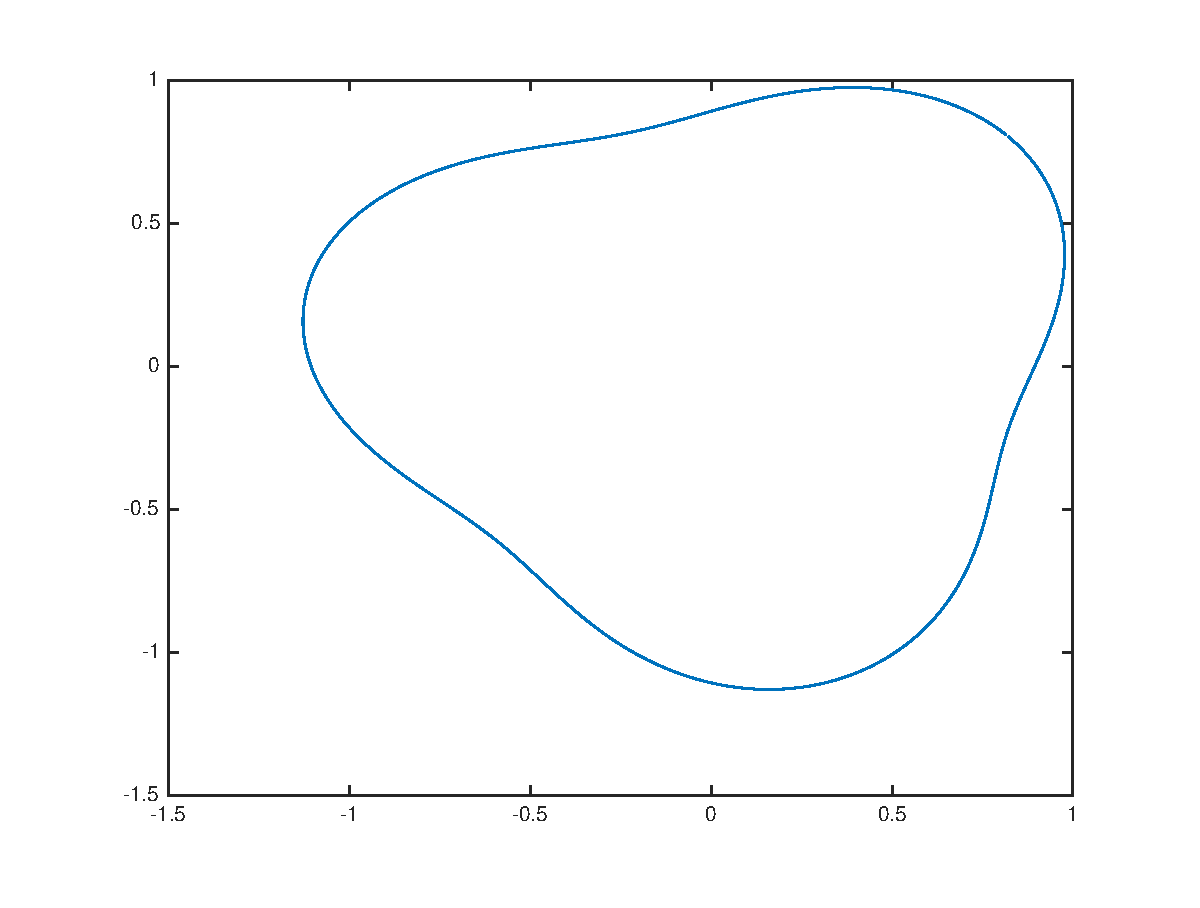
\includegraphics[width=0.48\textwidth]{./Img/figure_sc_elastic/pear.eps}
	\caption{散射系数实验中的障碍物形状:第一个是圆,第二个是梨形}\label{shape}
\end{figure}


为了比较不同角频率情况下,散射系数的逼近情况,我们分别取 $\omega= \pi,2\pi,4\pi,8\pi$。如图 \ref{figure_2}-\ref{figure_9} 所示,其中每一幅图对应某种形状的 $\mathbf{R}_\alpha^i(x;d) \ , \  \hat {\mathbf{R}}_\alpha^i(x;d,\nu(x)), \ \al=s,p,  \ i=1,2$ 的对比。
\begin{figure}[htbp]
	\centering
	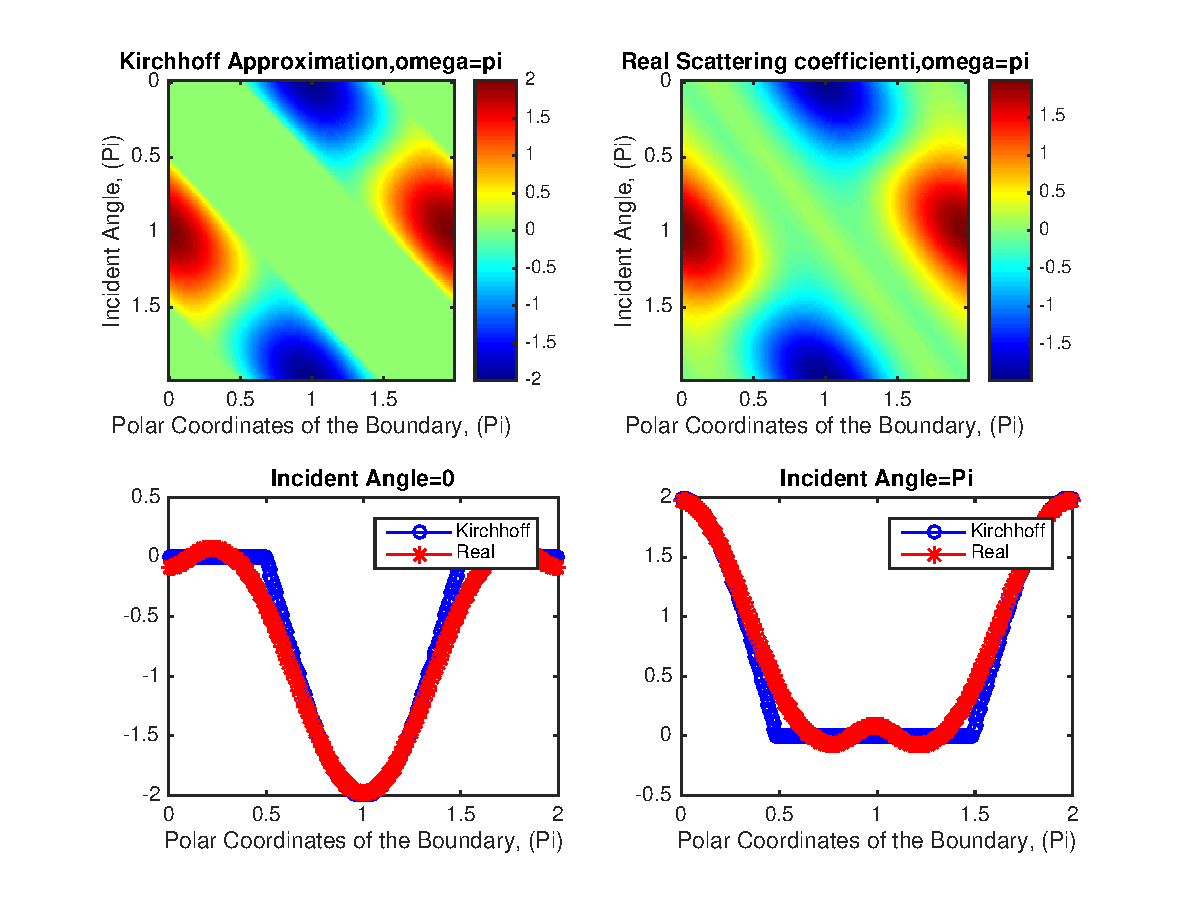
\includegraphics[width=0.48\textwidth]{./Img/figure_sc_elastic/sc_p1_circle_1.eps}
	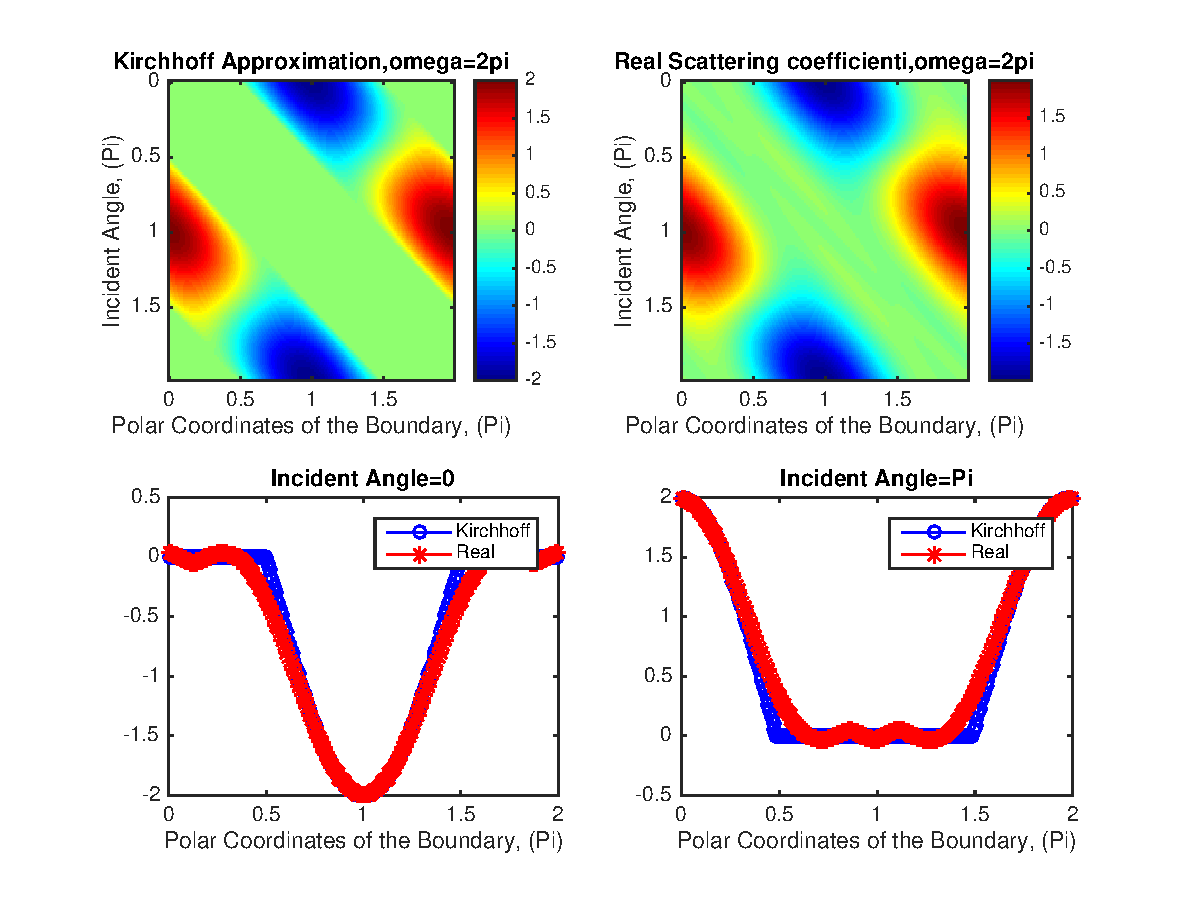
\includegraphics[width=0.48\textwidth]{./Img/figure_sc_elastic/sc_p1_circle_2.eps}
	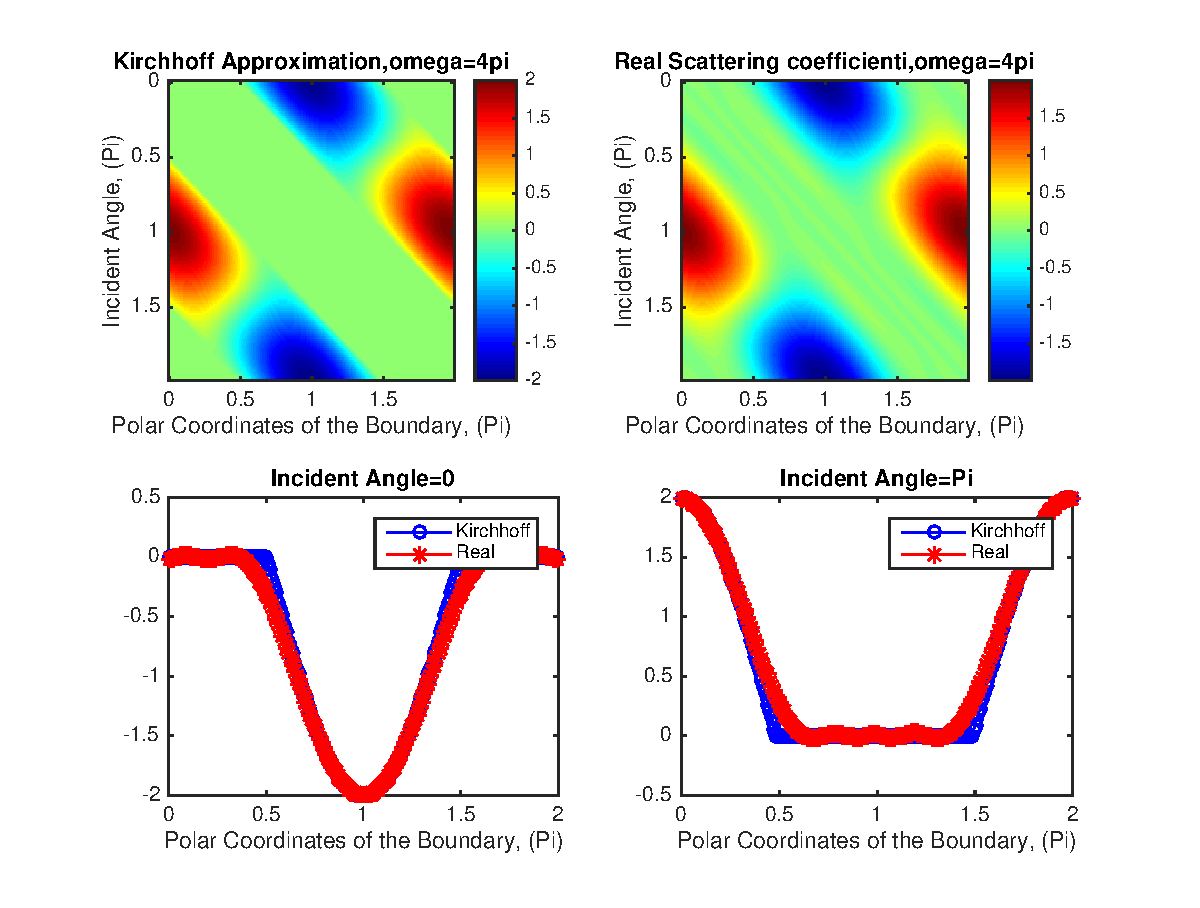
\includegraphics[width=0.48\textwidth]{./Img/figure_sc_elastic/sc_p1_circle_4.eps}
	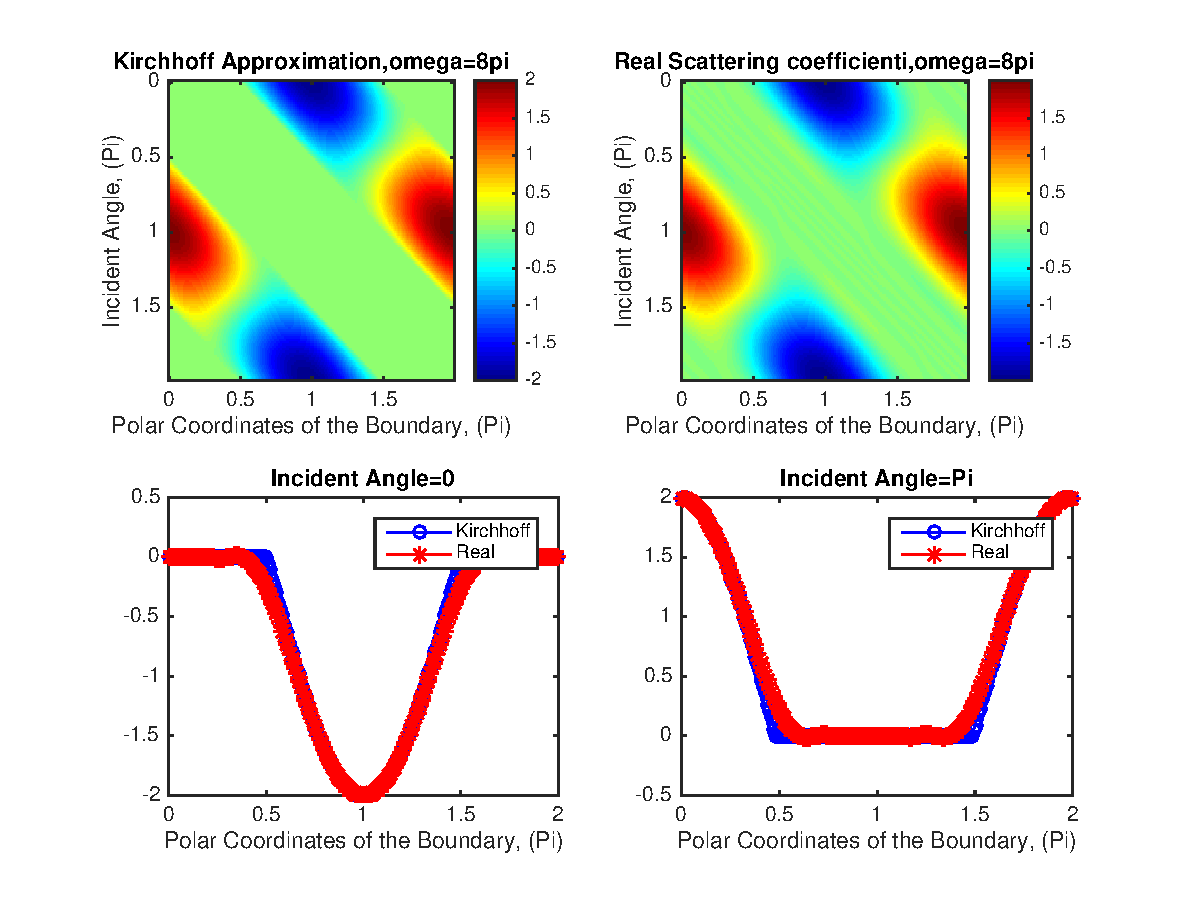
\includegraphics[width=0.48\textwidth]{./Img/figure_sc_elastic/sc_p1_circle_8.eps}		
	\caption{圆形的$\mathbf{R}_p^1$ 和 $\hat {\mathbf{R}}_p^1$ .}\label{figure_2}
\end{figure}

 每幅图含四幅针对不同角频率的子图, 每幅子图中第一行中的第一列代表真实的散射系数,第二列代表 Kirchhoff 逼近的散射系数; 第一行中的横坐标是边界的参数化 $\theta/2\pi$,纵坐标是入射方向 $t/2\pi$。第二行是入射角为 $0$ 和 $\pi$ 对于的图, 其中每幅图中红线代表真实的散射系数,蓝线代表 Kirchhoff 逼近的散射系数。
\begin{figure}[htbp]
	\centering
	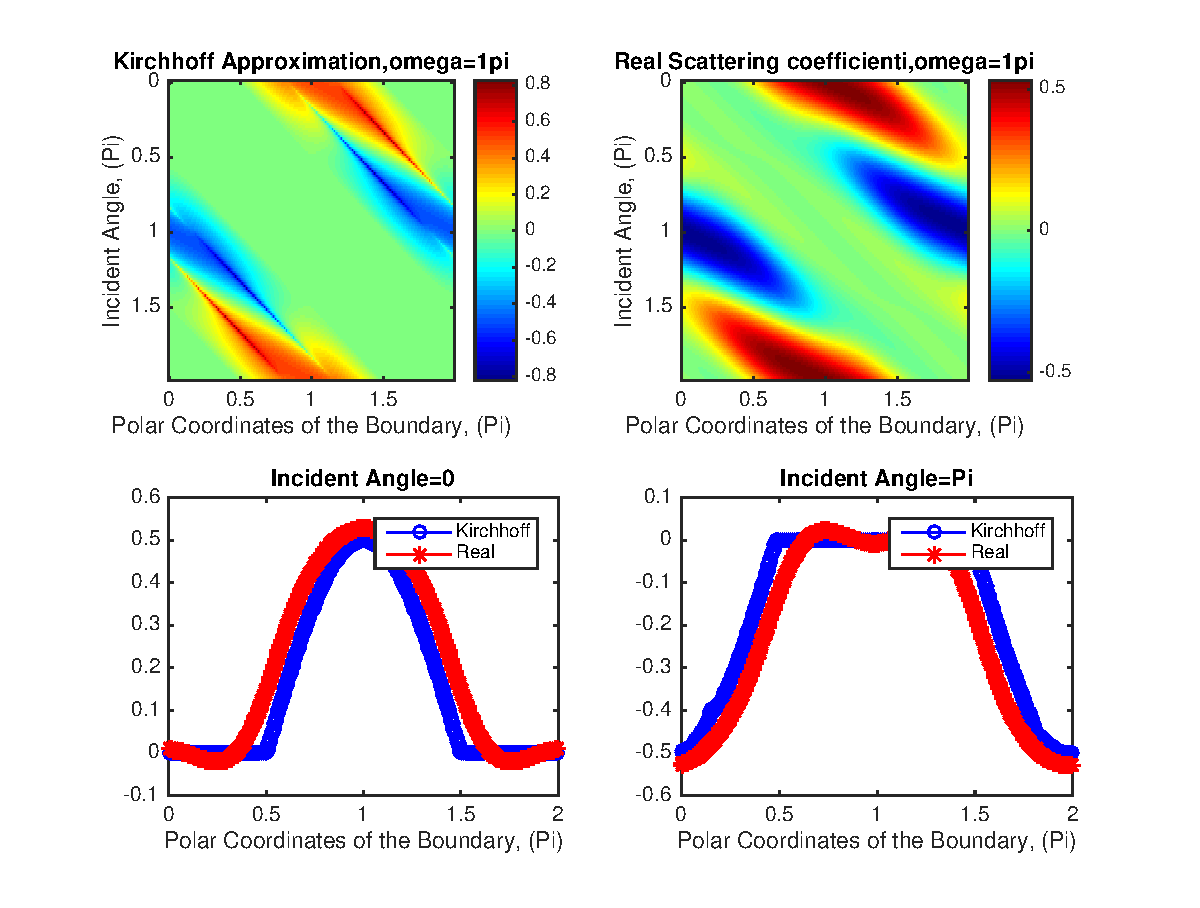
\includegraphics[width=0.48\textwidth]{./Img/figure_sc_elastic/sc_s2_circle_1.eps}
	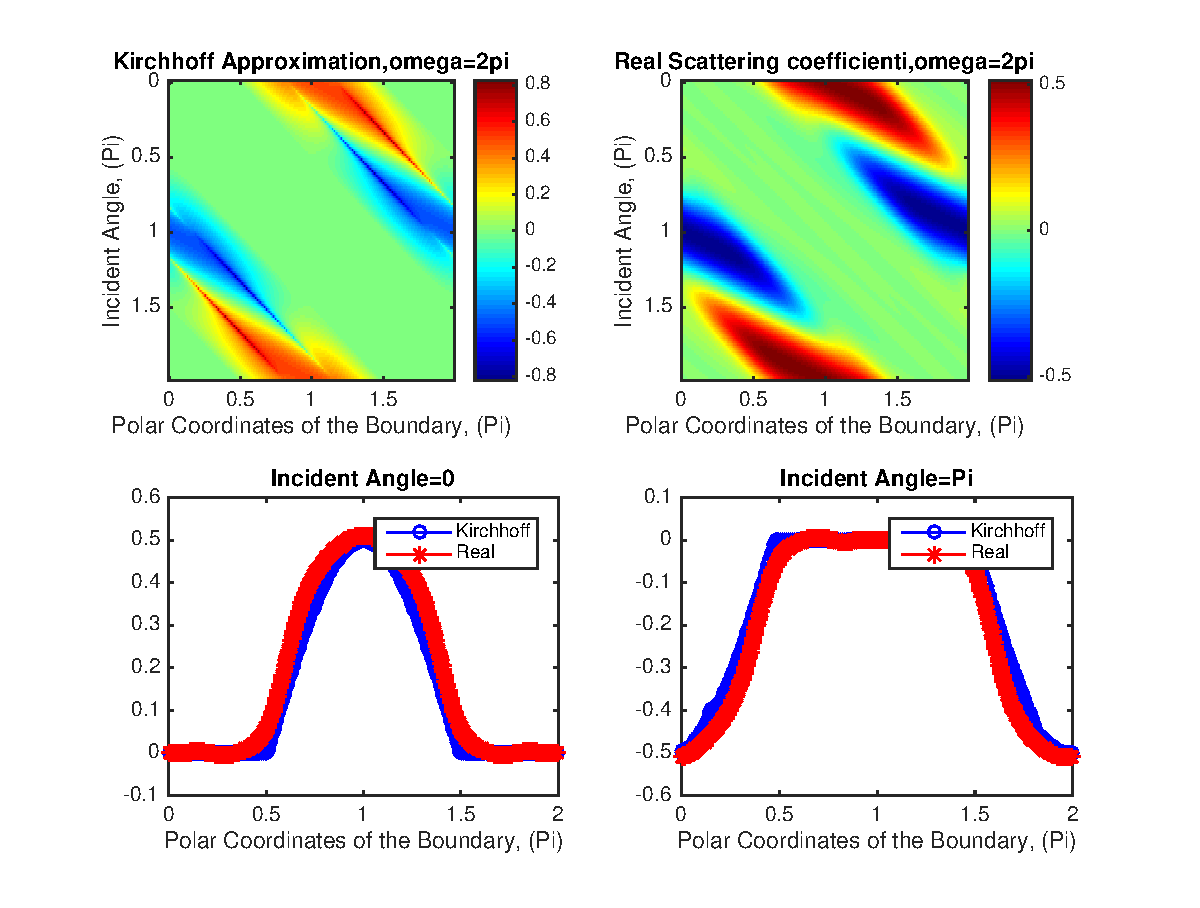
\includegraphics[width=0.48\textwidth]{./Img/figure_sc_elastic/sc_s2_circle_2.eps}
	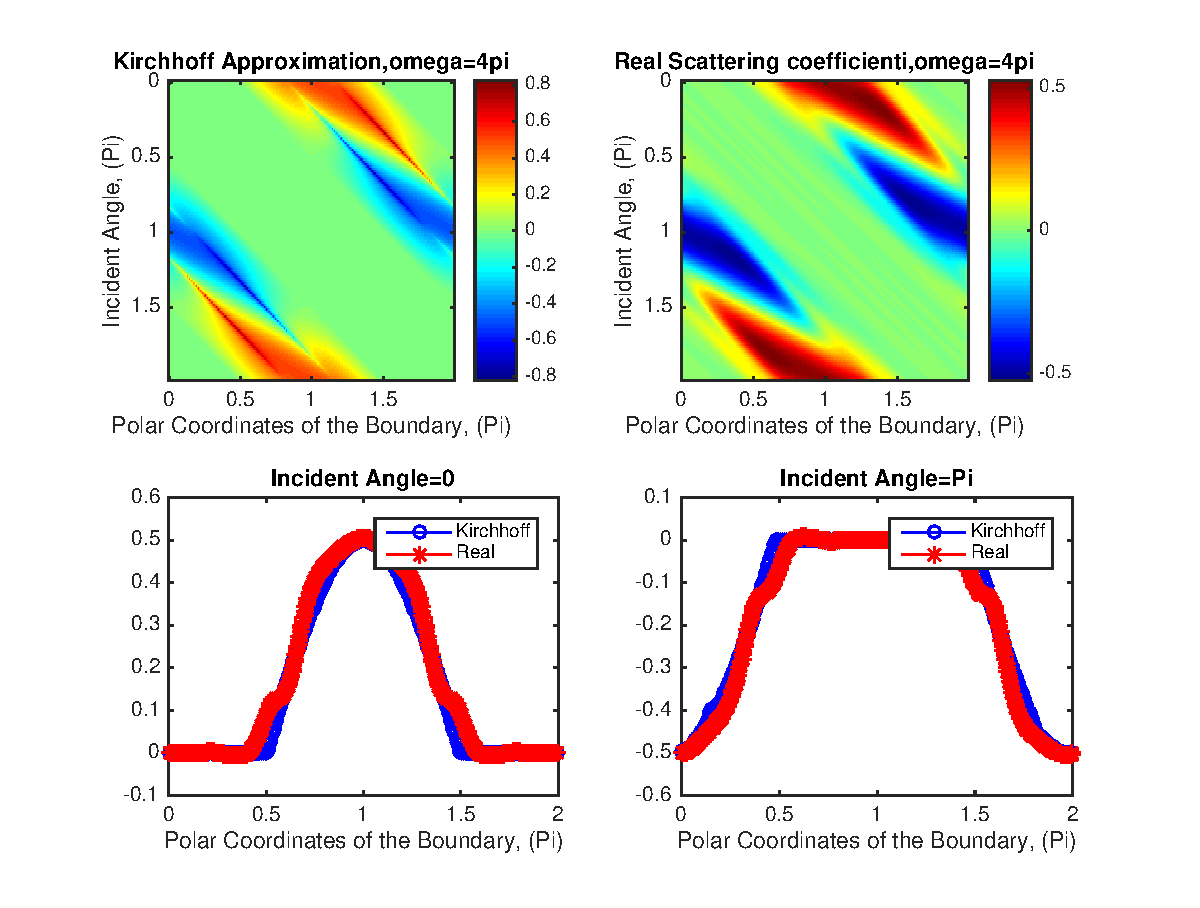
\includegraphics[width=0.48\textwidth]{./Img/figure_sc_elastic/sc_s2_circle_4.eps}
	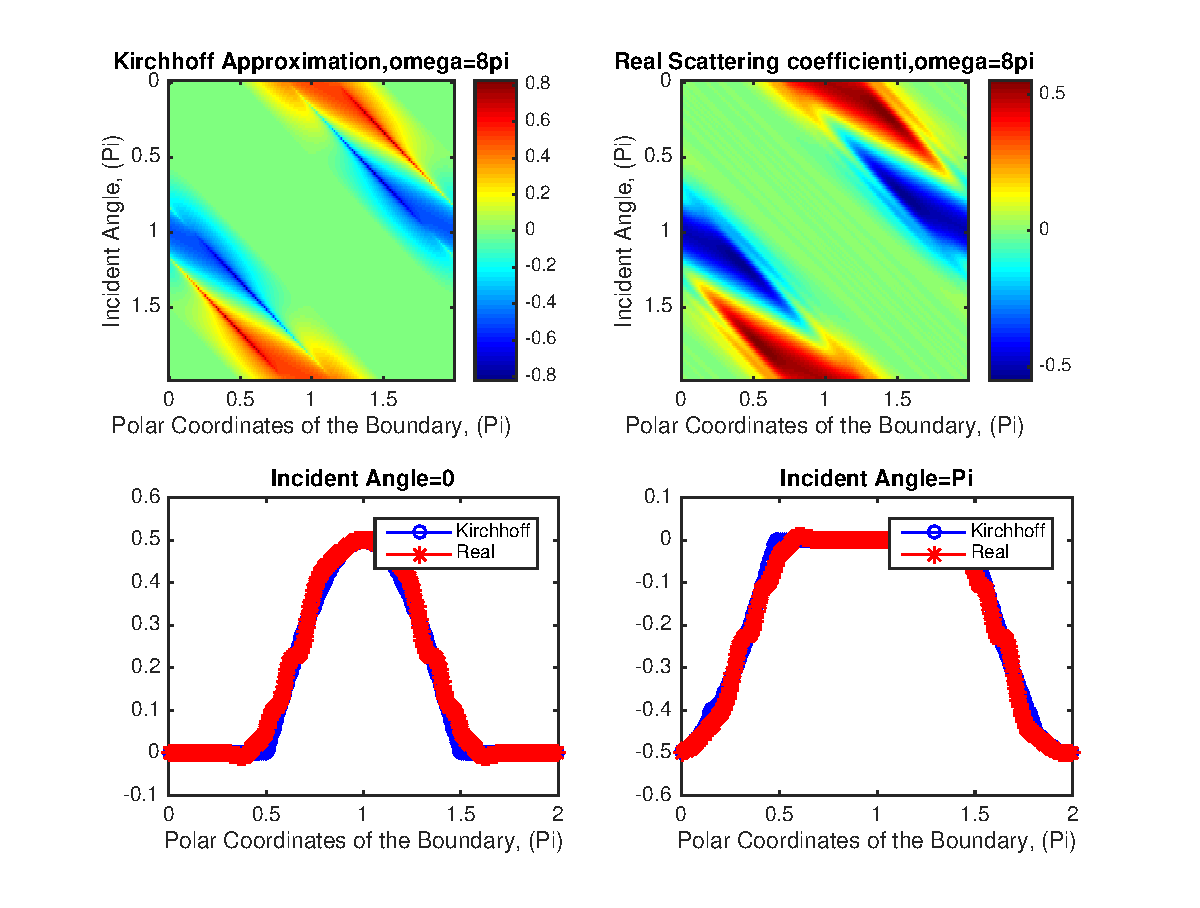
\includegraphics[width=0.48\textwidth]{./Img/figure_sc_elastic/sc_s2_circle_8.eps}		
	\caption{圆形的 $\mathbf{R}_s^2$ 和 $\hat {\mathbf{R}}_s^2$ }\label{figure_5}
\end{figure}
由图\ref{figure_2}-\ref{figure_9}, 我们可以看到, 当角频率比较大时,Kirchhoff 逼近 (\ref{kir}) 的效果是非常好, 符合高频光学近似。 然后, 我们发现当角频率不是很大的是, Kirchhoff 逼近的效果还是非常理想的。

\begin{figure}[htbp]
	\centering
	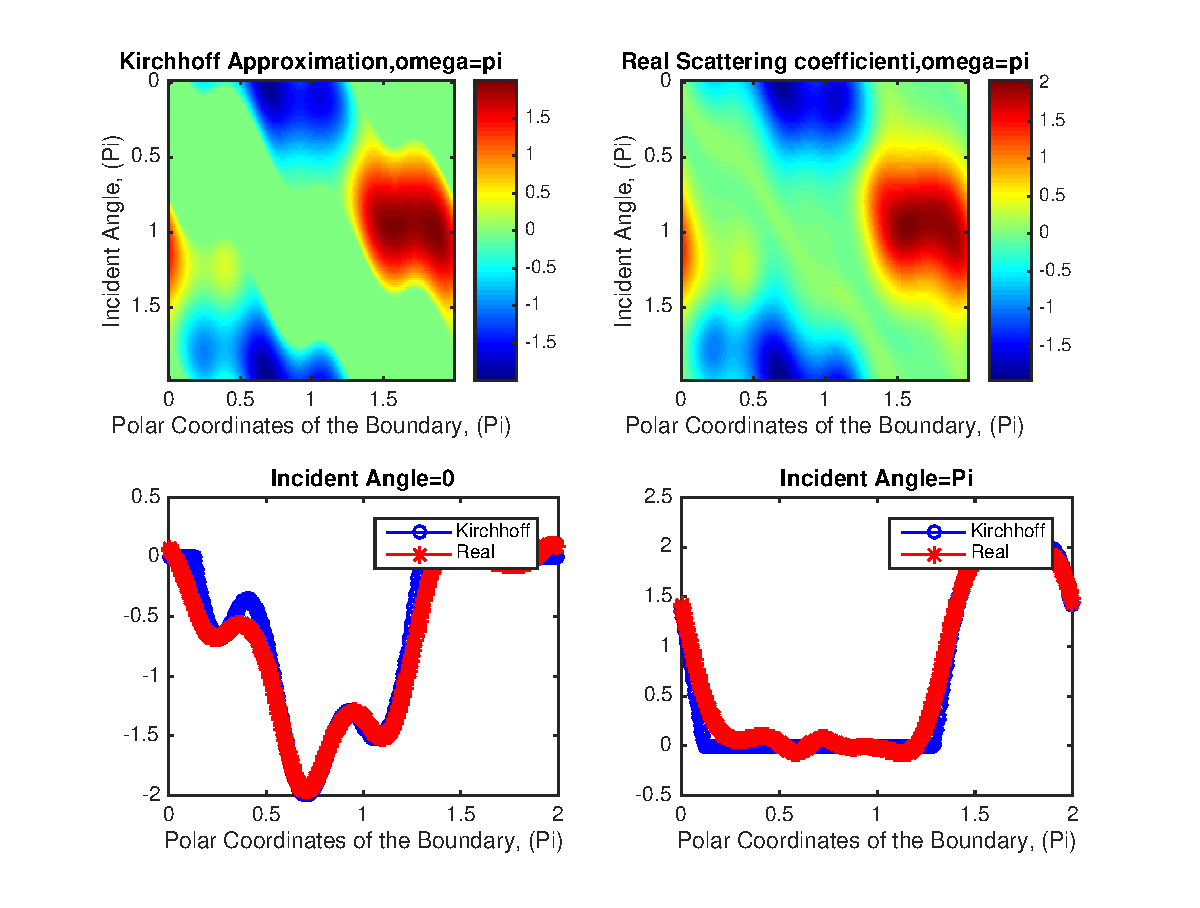
\includegraphics[width=0.48\textwidth]{./Img/figure_sc_elastic/sc_p1_pear_1.eps}
	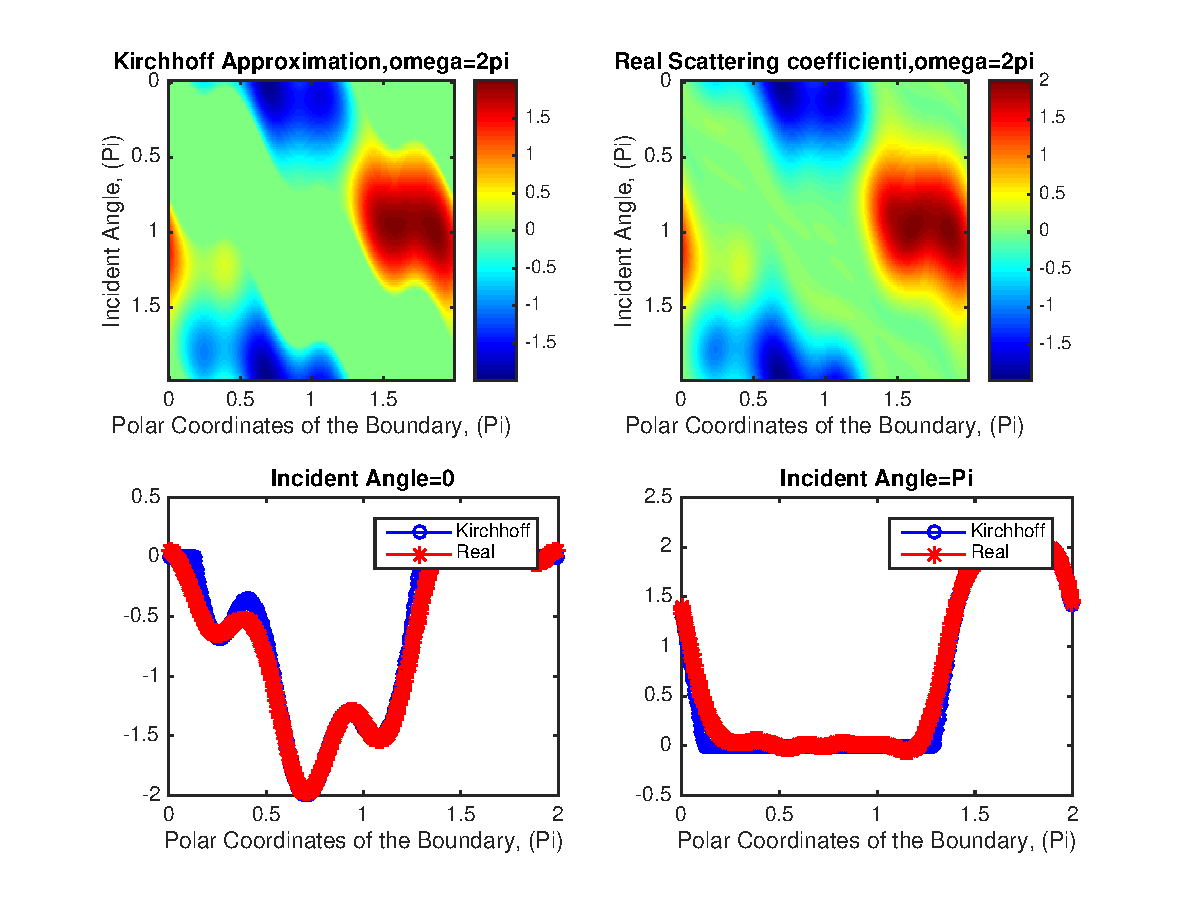
\includegraphics[width=0.48\textwidth]{./Img/figure_sc_elastic/sc_p1_pear_2.eps}
	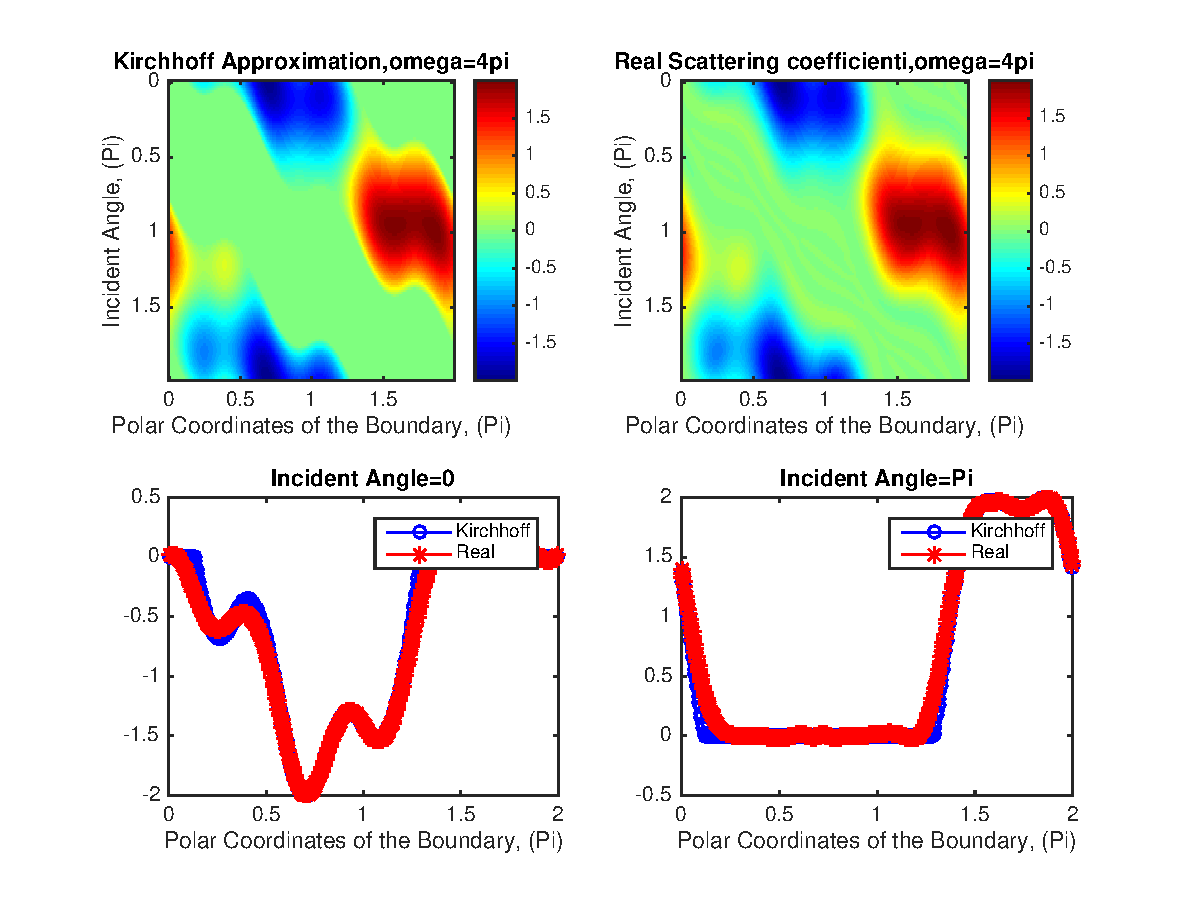
\includegraphics[width=0.48\textwidth]{./Img/figure_sc_elastic/sc_p1_pear_4.eps}
	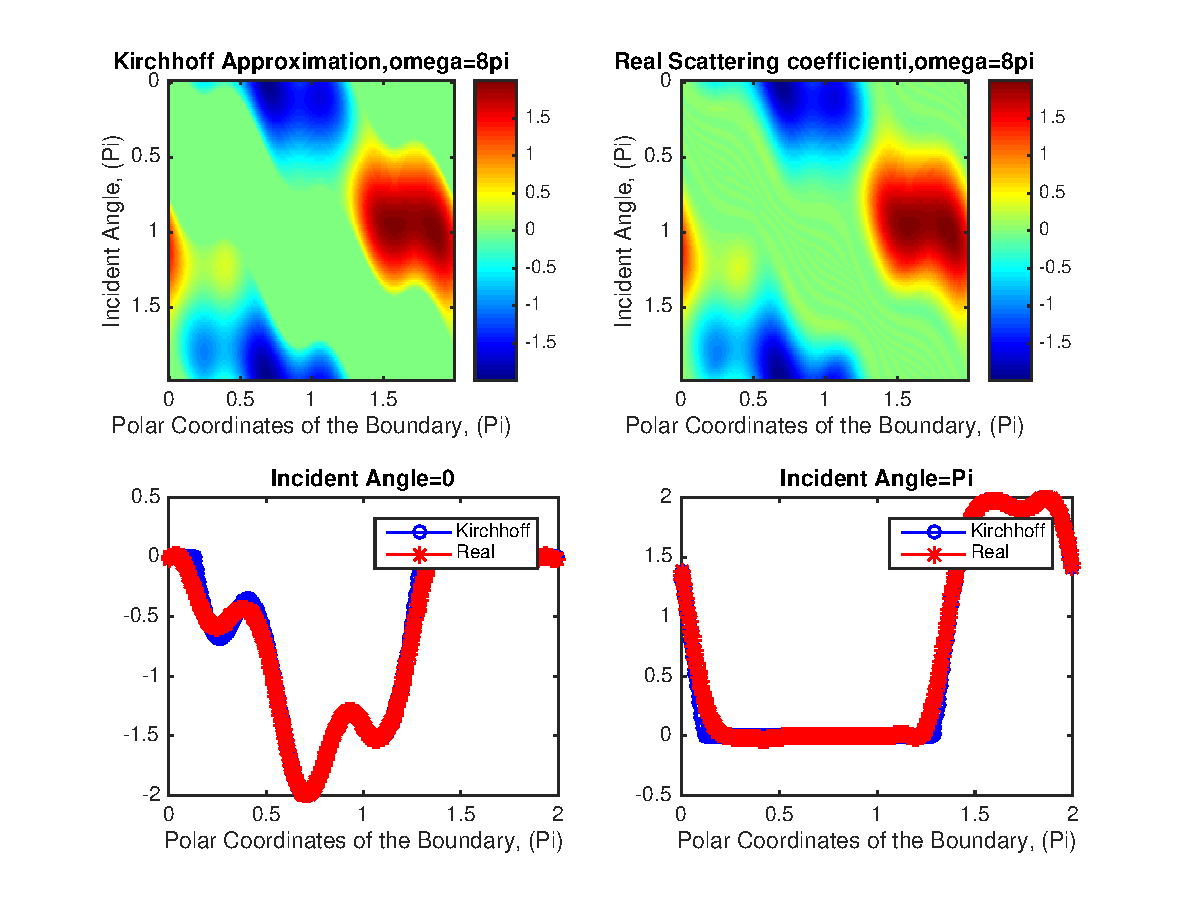
\includegraphics[width=0.48\textwidth]{./Img/figure_sc_elastic/sc_p1_pear_8.eps}		
	\caption{梨形的 $\mathbf{R}_p^1$ 和 $\hat {\mathbf{R}}_p^1$ }\label{figure_6}
\end{figure}



\begin{figure}[htbp]
	\centering
	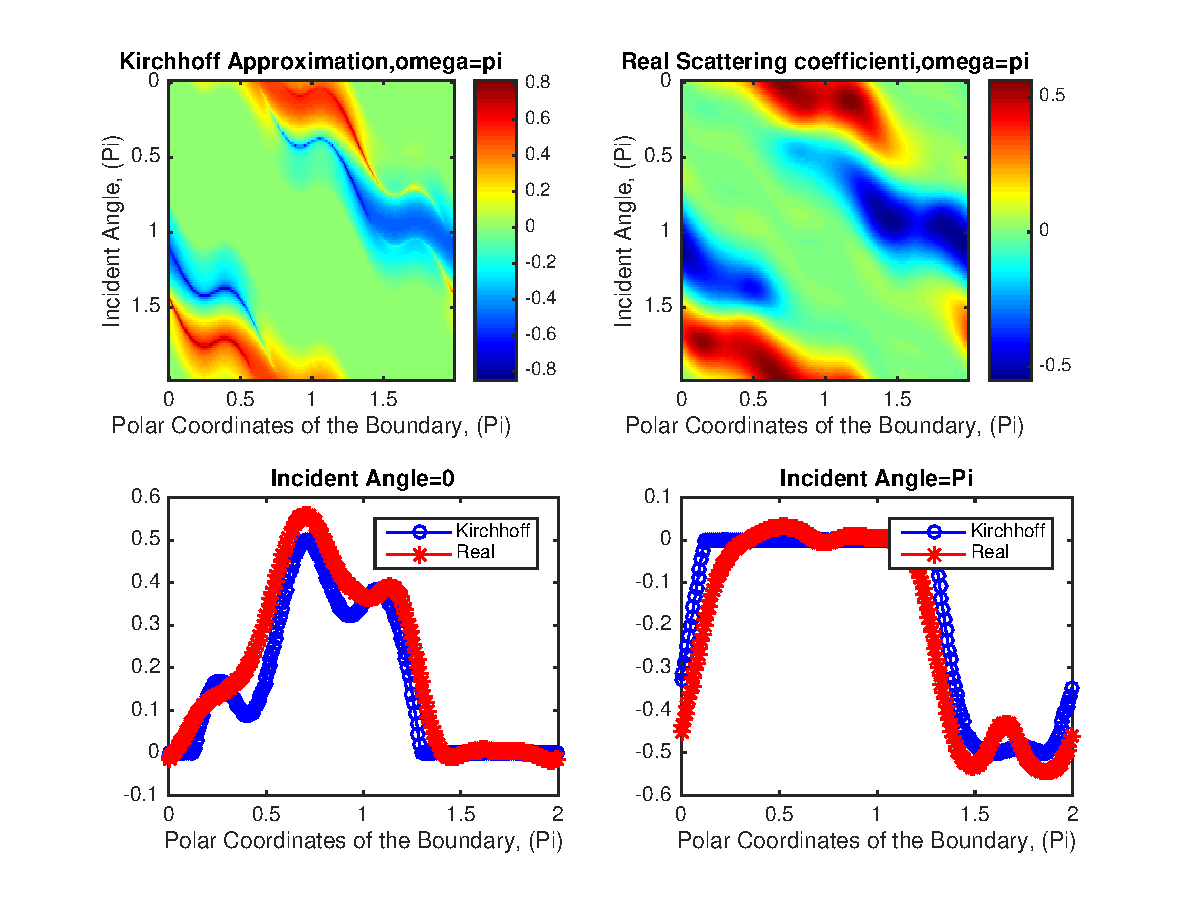
\includegraphics[width=0.48\textwidth]{./Img/figure_sc_elastic/sc_s2_pear_1.eps}
	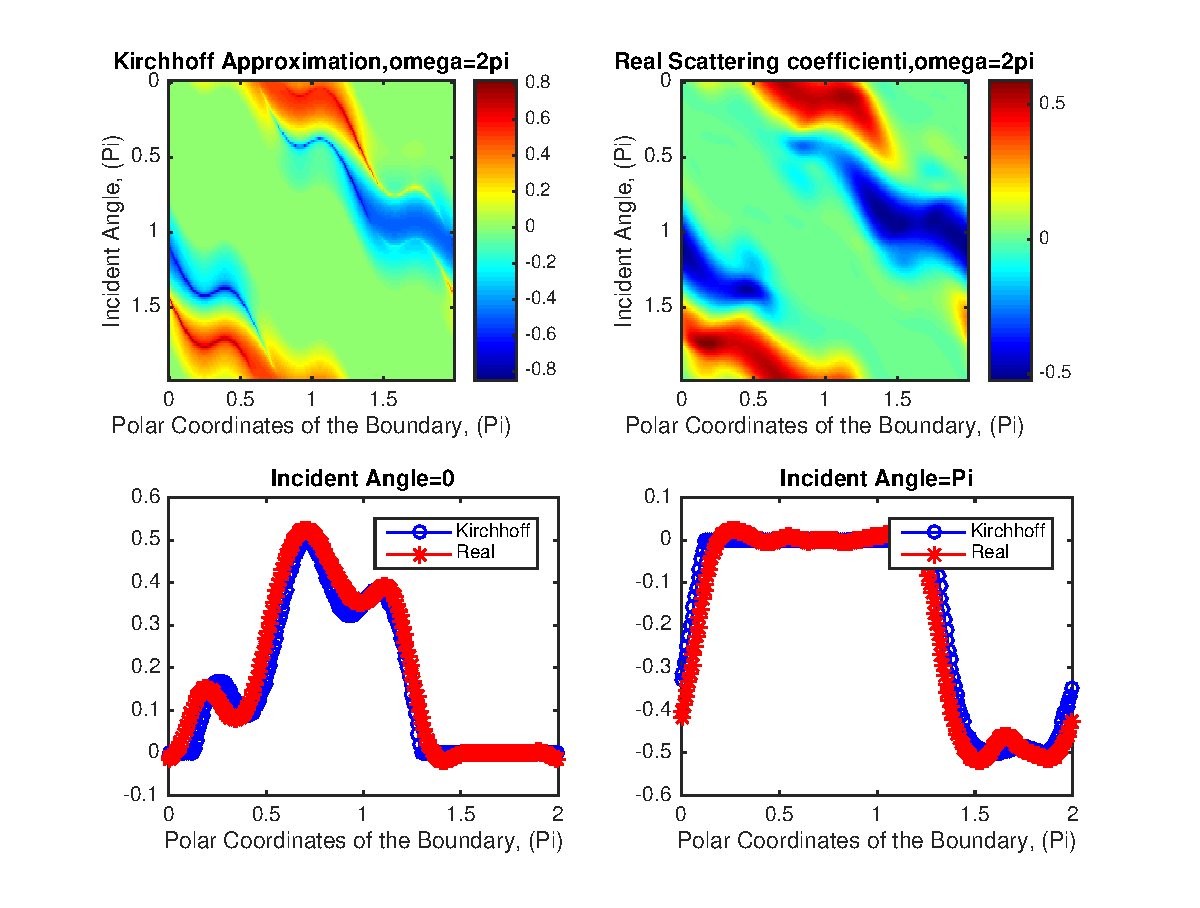
\includegraphics[width=0.48\textwidth]{./Img/figure_sc_elastic/sc_s2_pear_2.eps}
	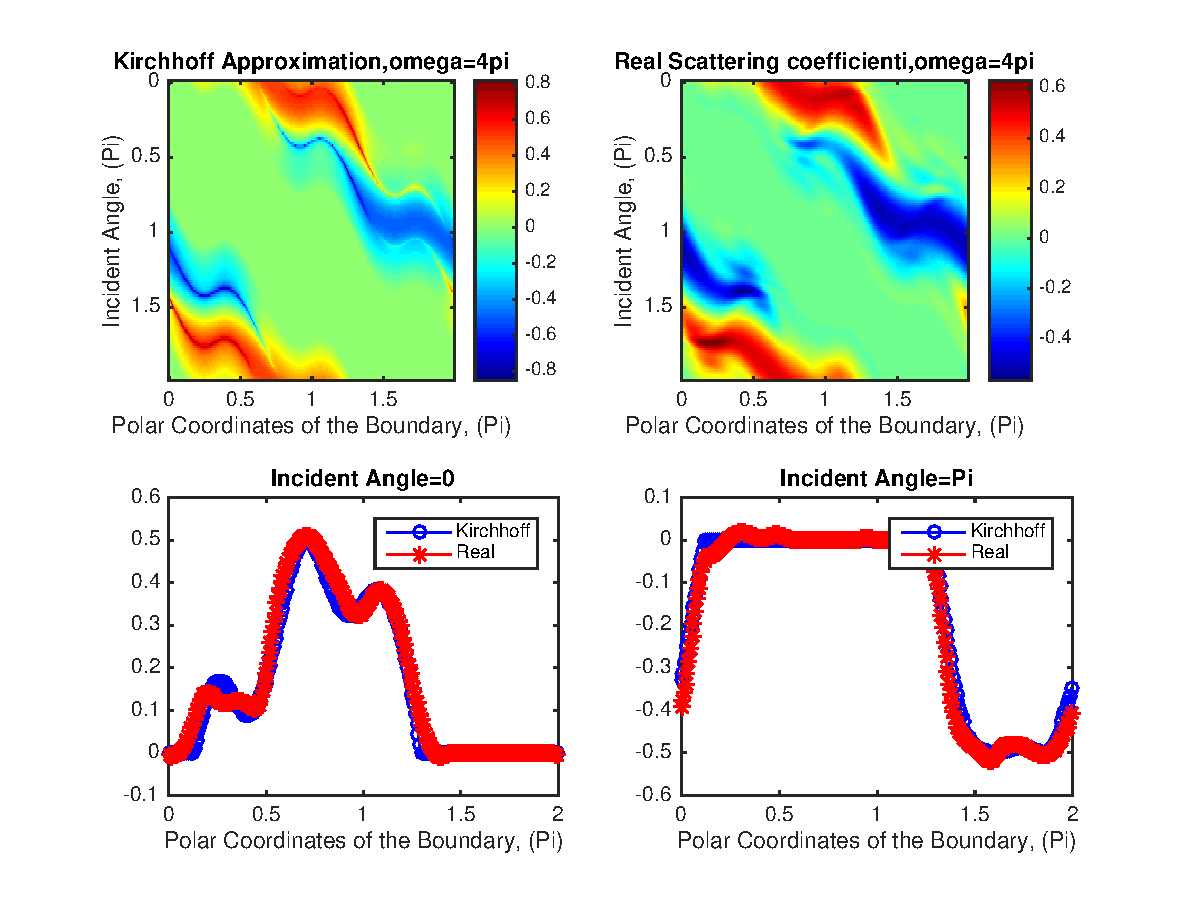
\includegraphics[width=0.48\textwidth]{./Img/figure_sc_elastic/sc_s2_pear_4.eps}
	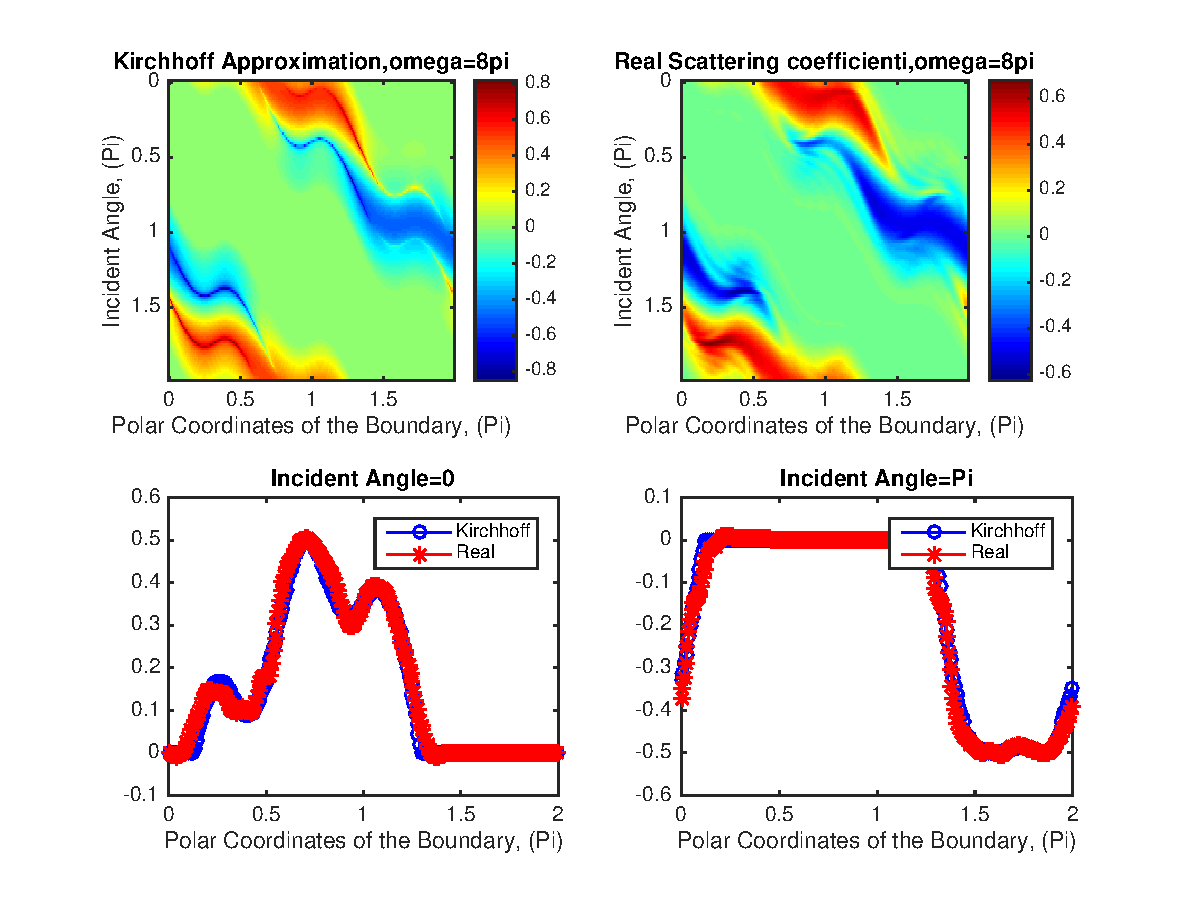
\includegraphics[width=0.48\textwidth]{./Img/figure_sc_elastic/sc_s2_pear_8.eps}		
	\caption{梨形的 $\mathbf{R}_s^2$ 和 $\hat {\mathbf{R}}_s^2$ }\label{figure_9}
\end{figure}



于是由式子 (\ref{F_theta})以及定理 \ref{thm:4.3}, 易得对于任意 $z\in\Ga_D$,
\ben
\hat I_d(z)&\approx&\Im\sum^2_{j=1}\int_{\Ga_D}\left[
\int^\pi_0\overline{\tilde A_j(\theta)}\i k_pR_p(x;\tau(\theta))e^{\i k_p(x-z)\cdot\tau(\theta)}d\theta\right]\cdot\overline{\F(z,x)}e_j ds(x)\\
& &+\Im\sum^2_{j=1}\int_{\Ga_D}\left[
\int^\pi_0\overline{\tilde B_j(\theta)}\i k_sR_s(x;\tau(\theta))e^{\i k_s(x-z)\cdot\tau(\theta)}d\theta\right]\cdot\overline{\F(z,x)}e_j ds(x).
\een
于是利用 Kirchhoff 有 
\be\label{sc4}
R_\alpha(x;\tau)\approx 0\ \ \mbox{if } x \in \Ga_D^{+}(\tau)=\{x\in \Ga_D, \nu(x)\cdot \tau>0\},\ \ \al=p,s.
\ee

 为了后文分析, 我们引入下面著名的驻相引理, 见  \cite[Theorem 7.7.5]{hor}.
 \begin{lem}\label{phase}
 	令振幅函数 $g\in C^2_0(\R)$ 及相函数 $f\in C^2(\R)$ 存在驻相点 $t_0$ ,即为 $f'(t_0)=0$, $f''(t_0)\not=0$, 且当 $t\not=t_0$ 时有 $f'(t)\not=0$ 。 于是对于任意 $\lambda>0$,存在常数 $C$ 成立
 	\ben
 	\left|\int_{\R}g(t)e^{\i\lambda f(t)}dt-g(t_0)e^{\i\lambda f(t_0)}\left(\frac{\lambda f''(t_0)}{2\pi\i}\right)^{-1/2}\right|
 	\le C\lambda^{-1}\|g''\|_{C(\R)}.
 	\een
 \end{lem}

 这里,我们假设障碍物 $D$ 是凸的 。令 $x(s)$, $0<s<L$, 是障碍物边界 $\Ga_D$ 的关于弧长的参数化表示。 定义 $x_{\pm}(\theta)$ 是边界 $\Ga_D$ 上满足 $\nu(x_\pm(\theta))=\pm\tau(\theta)$ 的点。令相函数 $f(s)= (x(s)-z)\cdot\tau(\theta)$ 且有 
 \ben
 f'(s)=x'(s)\cdot\tau(\theta),  \ \ f''(s)=x''(s) \cdot\tau(\theta).
 \een
 显然有 $f'(s_\pm)=\pm x'(s_\pm)\cdot\nu(x(s_\pm)), f''(s_\pm)=\pm x''(s_\pm)\cdot \nu(yx(s_\pm))= \pm\kappa(x(s_\pm))|x'(s_\pm)|^2$, 其中 $\kappa$ 表示 $\Ga_D$ 的曲率。
因此,利用驻相引理和 Kirchhoff 逼近 (\ref{sc4}) 我们可以得到:
\ben
\hat I_d(z)&\approx&\Im\sum^2_{j=1}\sqrt{2\pi k_p}
\int^\pi_0\overline{\tilde A_j(\theta)}e^{\i k_p(x_-(\theta)-z)\cdot\tau(\theta)+\i\frac\pi 4}\,\frac{R_p(x_-(\theta);\tau(\theta))\cdot\overline{\F(z,x_-(\theta))}e_j}{\sqrt{\kappa(x_-(\theta))}}d\theta\\
& &+\Im\sum^2_{j=1}\sqrt{2\pi k_s}
\int^\pi_0\overline{\tilde B_j(\theta)}e^{\i k_s(x_-(\theta)-z)\cdot\tau(\theta)+\i\frac\pi 4\,}\frac{R_s(x_-(\theta);\tau(\theta))
	\cdot\overline{\F(z,x_-(\theta))}e_j}{\sqrt{\kappa(x_-(\theta))}}d\theta.
\een
由于 $\nu(x_-(\theta))=-\tau(\theta)$, 通过 (\ref{kir_p}) 和 (\ref{kir_s}) 我们可以得到
\be\label{sc5}
& &R_p(x_-(\theta);\tau(\theta))\approx-2(\lam+2\mu)\tau(\theta),\ \ \\ 
\label{sc6} & &R_s(x_-(\theta);\tau(\theta))\approx-2\mu\tau(\theta)^\perp.
\ee

现在, 我们来观察边界 $\Ga_D$ 上的点 $z$。 当$\nu(z)\cdot\tau(\theta)>0$ 时,其中 $\theta\in (0,\pi)$, 此时 $z$ 点位于 $\Ga_D$ 背对于 $\Ga_0$ 的那一部分。同时,此时 $x_-(\theta)$ 位于 $\Ga_D$ 正对于 $\Ga_0$ 的那一部分。 于是, $z$ 距离 $x_-(\theta)$ 就较远, 因此得到 $\F(z,x_-(\theta))e_j\approx 0$, 然后有  $\hat{I}_d(z)\approx0$。 这就说明,只利用 $\Ga_0$ 上收集的数据无法将障碍物背对于 $\Ga_0$ 那部分成像, 而且这一结论在后文中的数值算例中也得到证实。 
另一方面, 如果 $z$ 位于 $\Ga_D$ 正对于 $\Ga_0$ 的阳面, 利用 (\ref{sc5}),(\ref{sc6}) , 我们可以发现 $\hat I_d(z)$ 正是 $[\kappa(x_-(\theta))]^{-1/2}$ 的加权和, 其中 $x_-(\theta)$ 在$\Ga_D$ 上 $z$ 附近的那部分点。综上所述, 成像函数 $\hat{I}_d(z)$ 可以将障碍物边界成像, 且仅能将障碍物的阳面成像。


\section{其它类型障碍物的RTM分辨率分析}
在这一节中, 我们将考虑在半空间弹性介质中利用 RTM 算法 \ref{alg_rtm} 来重构具有阻抗边界条件的不可穿透障碍物和可穿透障碍物。

对于具有阻抗边界的不可穿透的障碍物,我们接收到的测量数据为 $u_q(x_r,x_s)=u_q^s(x_r,x_s)+\N(x_r,x_s)q$, $q=e_1, e_2$, 其中 $u^s_q(x,x_s)$ 是如下半空间弹性波方程的散射解:
\ben
& &\Delta_e u^s_q(x,x_s) + \omega^2 u^s_q(x,x_s) =0\ \ \mbox{\rm in } \R^2_+\bks \bar{D}, \\
& &\sigma(u^s_q(x,x_s))\nu+\i\eta(x)u^s_q(x,x_s)=-[\sigma(\N(x,x_s)q)\nu+\i\eta(x)\N(x,x_s)q]\ \ \mbox{\rm on } \Ga_D, \\ 
& &\sigma(u^s_q(x,x_s))e_2=0 \ \ \mbox{\rm on } \Ga_0,
\een
这里在 $\Ga_D$ 上 $\eta\in L^\infty(\Ga_D)$ 以及 $\eta\ge 0$,特别地, 当 $\eta=0$ 时, 上面的障碍物边界条件对应的是 Neumann边界条件,因此这里我们不在单独讨论满足 Neumann 边界条件的障碍物。 对定理 \ref{thm:4.3} 稍作修改, 我们可以得到如下针对具有阻抗边界的不可穿透型障碍物的 RTM 方法的分辨率分析的定理, 这里我们不在赘述定理证明。
\begin{thm}\label{thm:5.1}
	对于任意 $z\in\Omega$, 令 $\U(z,x)\in\C^{2\times2}$, 其中 $\U(z,x)e_j$, $j=1,2$ 是如下弹性波方程的散射解:
	\ben
	\hskip-1cm& & \Delta_e[\U(z,x)e_j]+ \omega^2[\U(z,x) e_j]= 0 \ \ \mbox{\rm in }\R^2\bks \bar{D},\\
	\hskip-1cm& &\sigma(\U(z,x)e_j)\nu+\i\eta(x)[\U(z,x)e_j]= -[\sigma(\overline{\F(z,x)}e_j)\nu+\i\eta(x)\overline{\F(z,x)}e_j ]\ \ \mbox{\rm on} \ \Ga_D.
	\een
	于是针对具有阻抗边界的不可穿透障碍物的散射数据 $u^s_q(x_r,x_s)$,RTM 成像函数(\ref{cor2}) 有如下表示
	\ben
	\hat{I}_d(z)&=&-\Im\sum_{j=1}^2\int_{\Gamma_D} [\U(z,x)e_j+\overline{\F(z,x)}e_j]\cdot[\sigma(\overline{\F(z,x)}e_j)\nu+\i\eta(x)\overline{\F(z,x)}e_j]ds(x)\ \\
	& &+R_d(z),\ \ \ \ \ \ \ \ \forall z\in\Om,
	\een
	这里 $|R_d(z)|\leq C\mu^{-2}(1+k_s d_D)^3\left[\left(\frac hd\right)^{2}+(k_sh)^{-1/4}\right]$ 其中常数 $C$ 仅依赖于 $\kappa$ 而与 $k_s,k_p, h, d, d_D$ 无关。
\end{thm}

对于可穿透型障碍物, 我们接收到的测量数据为 $u_q(x_r.x_s)=u_q^s(x_r,x_s)+\N(x_r,x_s)q$, $q=e_1,e_2$, 其中 $u^s_q(x,x_s)$ 是如下弹性波方程的散射解:
\ben
& &\Delta_e u^s_q(x,x_s) + \omega^2n(x) u^s_q(x,x_s) =-\om^2(n(x)-1)\N(x,x_s)q\ \ \mbox{\rm in } \R^2_+, \\
& &\sigma(u^s_q(x,x_s))e_2=0 \ \ \mbox{\rm on }\Ga_0, 
\een
这里 $n(x)\in L^{\infty}({\R^2_+})$ 是正函数,且当 $x\notin D$ 时,$n(x)==1$。类似地, 对定理 \ref{thm:4.3} 稍作修改, 我们可以得到如下针对可穿透型障碍物的 RTM 方法的分辨率分析的定理, 这里我们不在赘述定理证明。

\begin{thm}\label{resolution2}
	对于 $z\in\Omega$, 令 $\U(z,x)\in\C^{2\times2}$ 其中 $\U(z,x)e_j$, $j=1,2$ 是如下弹性波方程的散射解:
	\ben
	& & \Delta_e [\U(z,x)e_j] + \omega^2n(x)[\U(z,x)e_j]= -\omega^2(n(x)-1)\overline{\F(z,x)}e_j \ \ \mbox{\rm in }\R^2.
	\een
	于是针对可穿透型障碍物的散射数据 $u^s_q(x_r,x_s)$,RTM 成像函数(\ref{cor2}) 有如下表示
	\ben
	\hat{I}_d(z)=\Im\sum_{j=1}^2 \int_{D}\omega^2(n(x)-1)[(\U(z,x)e_j+\overline{\F(z,x)}e_j)\cdot\overline{\F(z,x)}e_j]dx+R_d(z),
	\een
	这里 $|R_d(z)|\leq C\mu^{-2}(1+k_s d_D)^3\left[\left(\frac hd\right)^{2}+(k_sh)^{-1/4}\right]$ 其中常数 $C$ 仅依赖于 $\kappa$ 而与 $k_s,k_p, h, d, d_D$ 无关。
\end{thm}


\section{数值测试}

在这一节中, 我们将呈现若干数值实验来展示 
RTM 算法的有效性。 为了合成散射数据, 我们对要计算的半空间弹性波方程的散射解 $u^s_q(x,x_s)$ 表示成以 Neumann Green 函数 $\N(x,y)$ 为积分核的单层位势,然后通过 Dirichlet 边界条件,与入射波 $u^i_q(x,x_s)$ 组合成边界积分方程。
由于当$ x=y$ 时,Neumann Green 函数 $\N(x,y)$ 只具有弱奇异性,即$\log |x-y|$。于是, 我们可以利用 Nystr\"{o}m 方法 \cite{colton-kress} 来离散边界 $\Ga_D$ 上的积分方程。 针对边界的离散剖分, 我们采用一致网格, 且每一个 p 入射波长均匀设置 10 个网格点。发射器和接收器均匀地分布在 $\Ga_d$ 上, 且对于所有数值实验, 都取 $h = 10, d = 50$ 及 {Lam\'{e}} 常数 $\lambda=1/2$, $\mu=1/4$。 下面实验中的各种障碍物形状, 其边界参数化表示如下: 
\ben
\mbox{圆形:}\ \ \ \ &&x_1=\rho\cos(\theta),\ \ x_2=\rho\sin(\theta);\ \ \\
\mbox{风筝形:}\ \ \ \ &&x_1=\cos(\theta) + 0.65\cos(2\theta) - 0.65,\ \ x_2=1.5 \sin (\theta);\ \ \\
\mbox{$p$-叶形:}\ \ \ \ &&r(\theta)=1+0.2\cos(p\theta); \\
\mbox{花生形:}\ \ \ \ &&x_1 = \cos \theta + 0:2 \cos 3\theta; x_2 = \sin \theta + 0:2 \sin 3\theta; \\
\mbox{方形:}\ \ \ \ &&x_1 = \cos3 \theta + \cos \theta; x_2 = \sin3\theta + \sin \theta.
\een
这里
$\theta\in[0,2\pi]$。且这里的数值成像函数为:
\ben
I_d(z)=\Im\sum_{q=e_1,e_2}\left\{\frac{|\Gamma_0^d|^2}{N_sN_r}\sum^{N_s}_{s=1}\sum^{N_r}_{r=1}
[\T_D(x_s,z)^Tq]\cdot[\T_D(x_r,z)^T\overline{u^s_q(x_r,x_s)}]\right\}.
\een

\bigskip

在下文中,我们所谓的 Dirichlet, Neumann 或是阻抗 (Impedance) 障碍物, 就意味着该障碍物是不可穿透的,而且其边界 $\Ga_D$ 满足 Dirichlet, Neumann 或是 阻抗边界条件。


\bigskip
\textbf{算例 1}. 这里我们只考虑  Dirichlet 障碍物来成像, 而变量是障碍物的形状, 包括圆形,花生形,四叶草形 以及旋转后的方形。 同样地, 
我们考虑针对 Dirichlet 障碍物,  Neumann 障碍物, 阻抗障碍物, 以及可穿透障碍物进行成像。 每个成像区域都为 $\Om=(-2,2) \times (8, 12)$ 且其样本点网格取为 $201 \times 201$。 我们设置发射器和接收器数量为 $N_s = N_r = 401$。 这里针对单频, 我们取角频率 $\om = 3\pi,4\pi$ ; 针对多频,取 $\om=\pi\times[2:0.5:8]$ ,再将成像函数值叠加。
\begin{figure}[htbp]
	\centering
	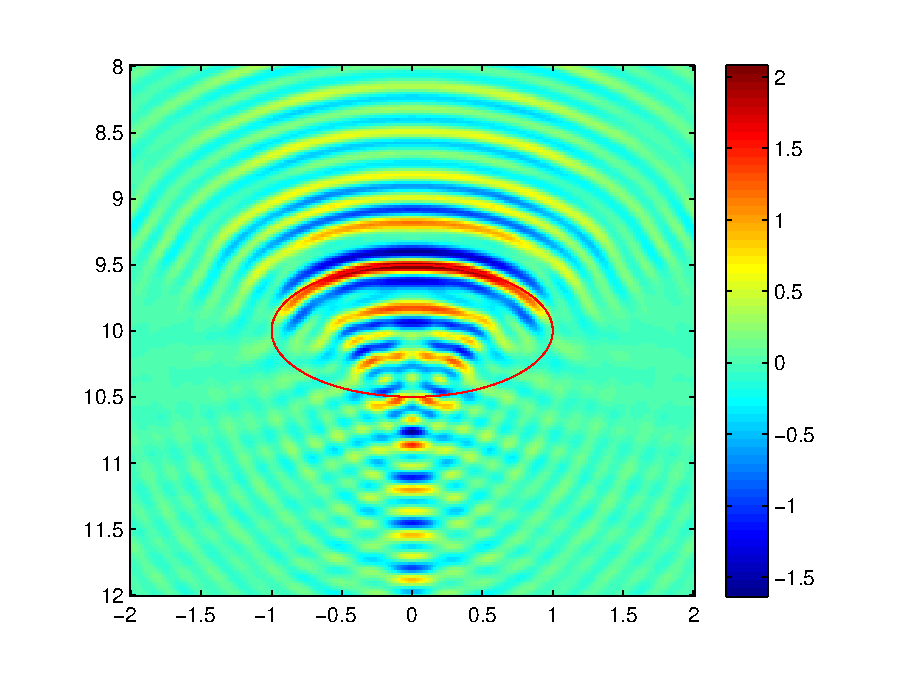
\includegraphics[width=0.32\textwidth]{./Img/graphic/circle_3pi.eps}
	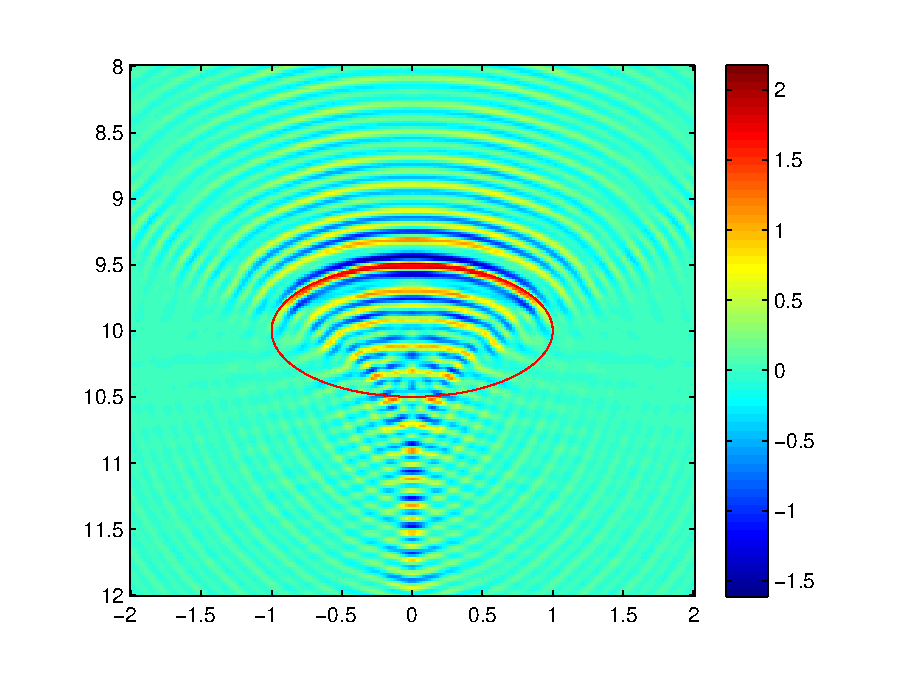
\includegraphics[width=0.32\textwidth]{./Img/graphic/circle_5pi.eps}
	\includegraphics[width=0.32\textwidth]{./Img/graphic/circle.eps}
	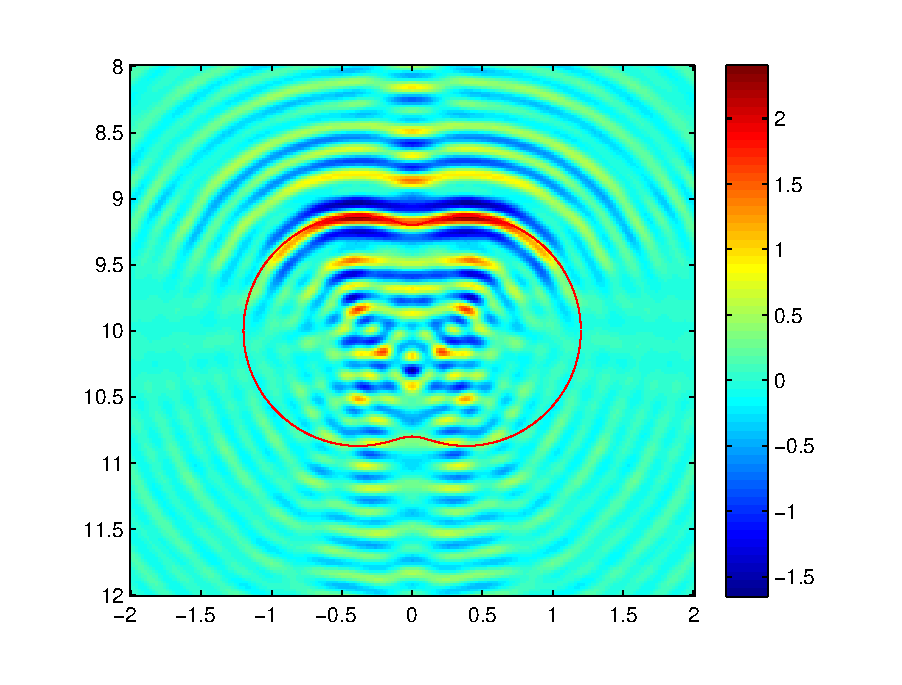
\includegraphics[width=0.32\textwidth]{./Img/graphic/peanut_3pi.eps}
	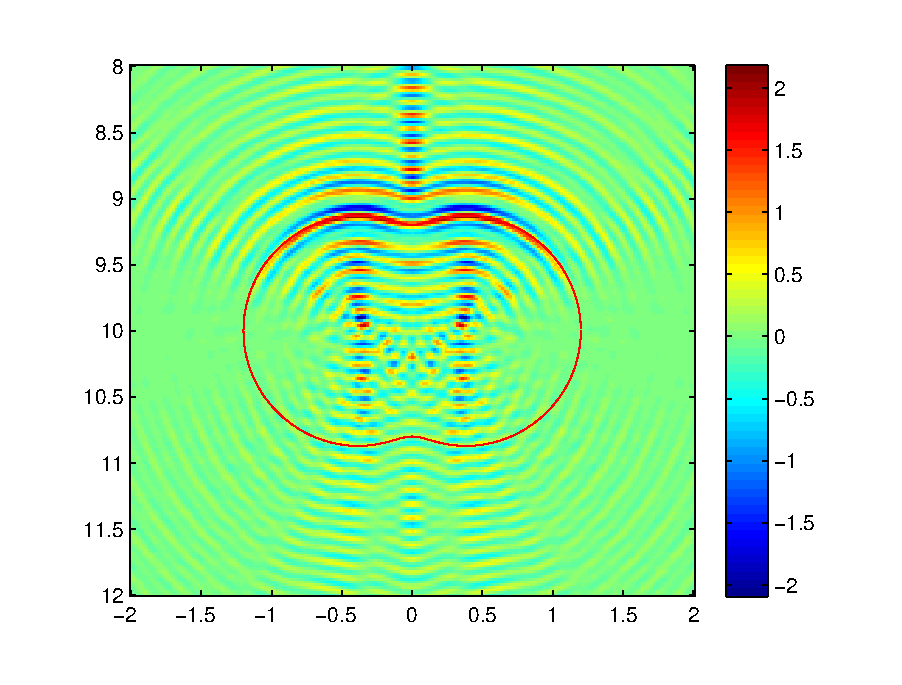
\includegraphics[width=0.32\textwidth]{./Img/graphic/peanut_5pi.eps}
	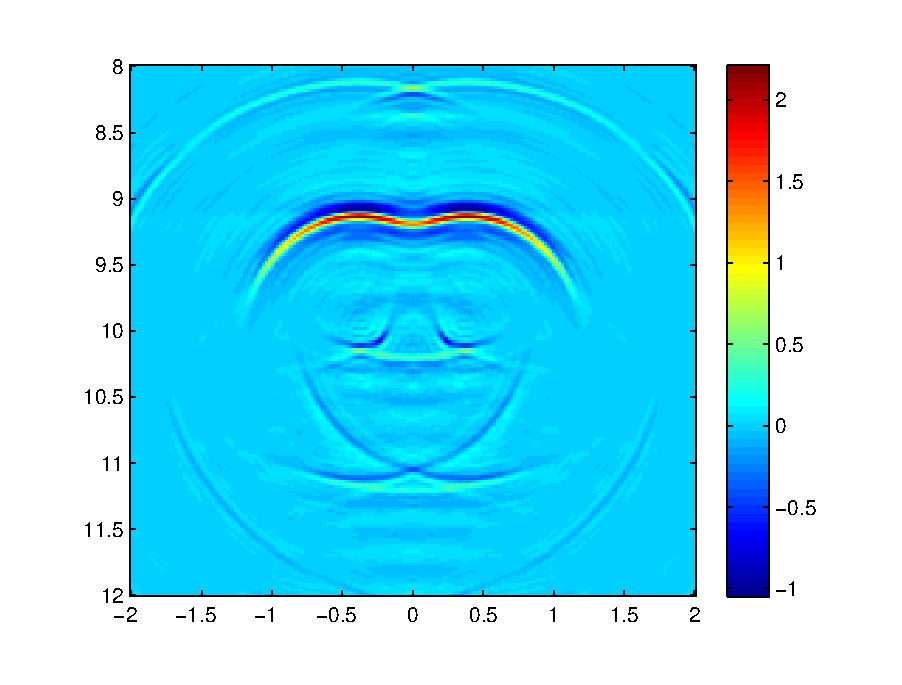
\includegraphics[width=0.32\textwidth]{./Img/graphic/peanut.eps}
	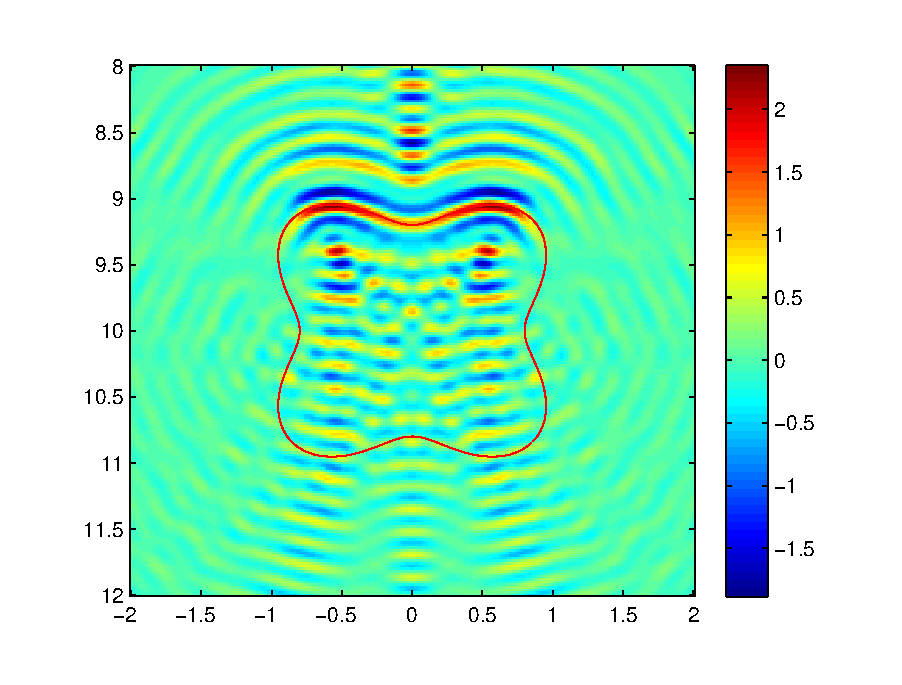
\includegraphics[width=0.32\textwidth]{./Img/graphic/p_leaf_3pi.eps}
	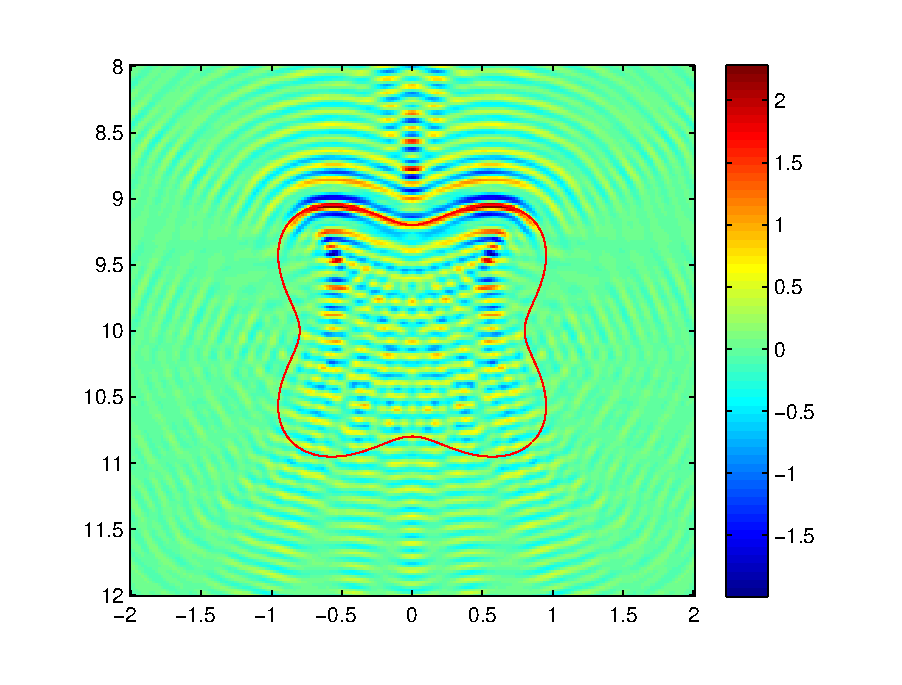
\includegraphics[width=0.32\textwidth]{./Img/graphic/p_leaf_5pi.eps}
	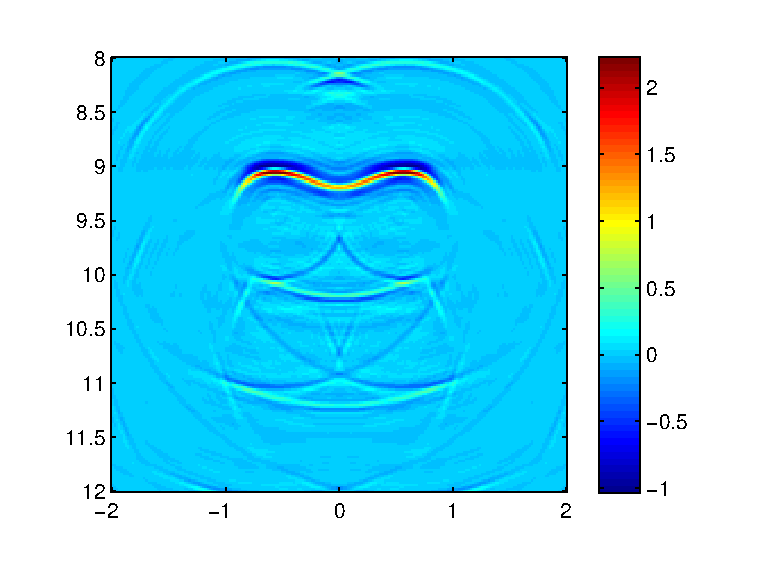
\includegraphics[width=0.32\textwidth]{./Img/graphic/p_leaf.eps}
	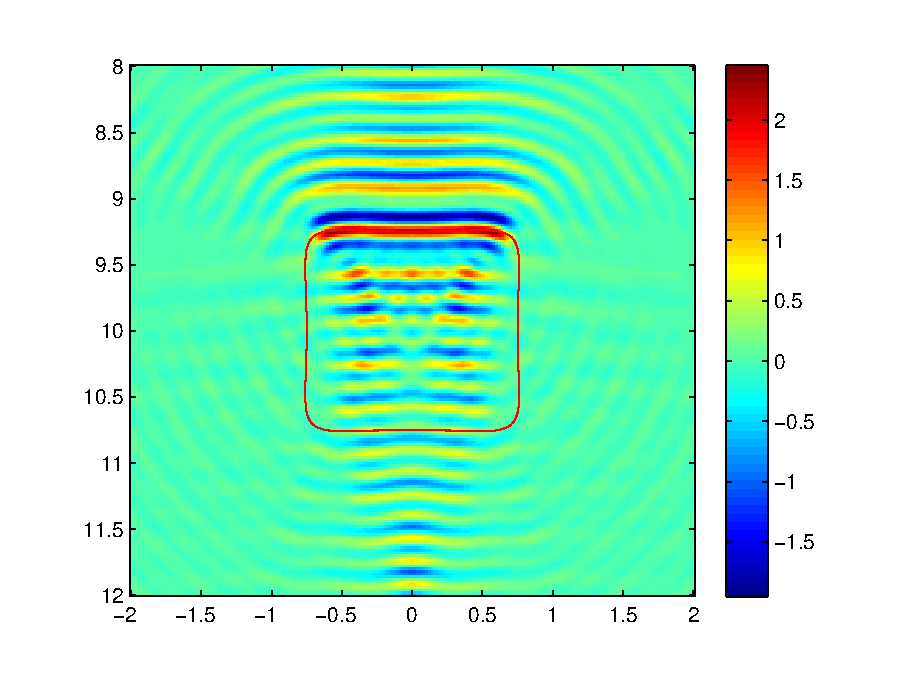
\includegraphics[width=0.32\textwidth]{./Img/graphic/rectangle_3pi.eps}
	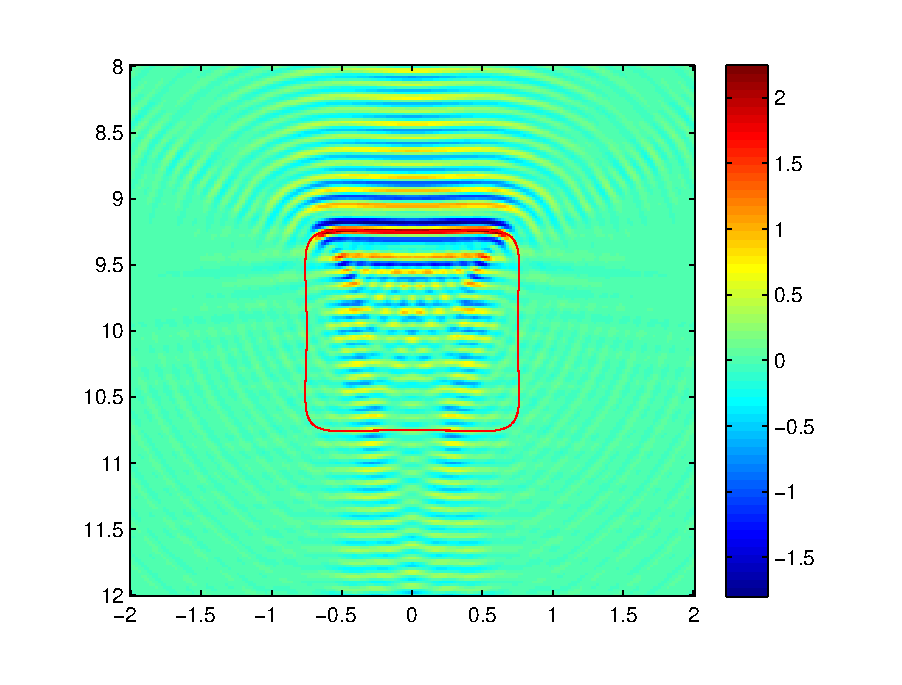
\includegraphics[width=0.32\textwidth]{./Img/graphic/rectangle_5pi.eps}
	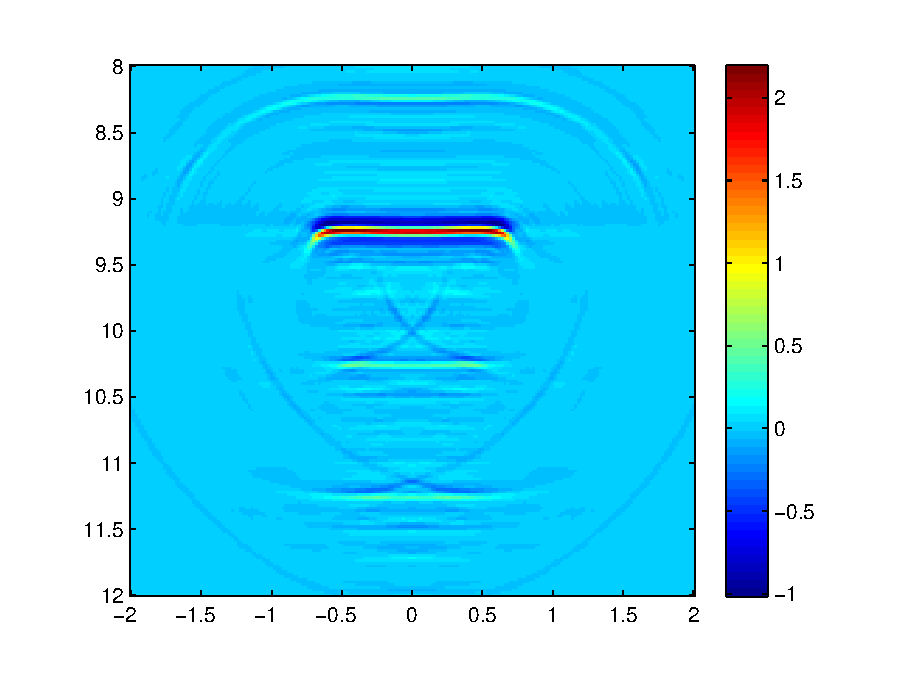
\includegraphics[width=0.32\textwidth]{./Img/graphic/rectangle.eps}
	
	\caption{算例 1: 从上到下是不同形状的 Dirichlet 障碍物,依次是圆形,花生形,四叶草形 以及旋转后的方形的成像结果。 其中,第一列是关于单频的, 其角频率为 $\om=3\pi$, 第二列是关于单频的, 其角频率为 $\om=5\pi$ 以及第三列是关于多频叠加的}\label{figure_21}
\end{figure}
如图 \ref{figure_21}, 针对不同形状的障碍物, RTM 算法都可以将其上沿给成像出来。 而且, 当对多个单频成像进行叠加后得到的多频成像结果可以显著提高单频的成像效果。

\bigskip
\textbf{算例 2}.
我们考虑针对 Dirichlet 障碍物,  Neumann 障碍物, 阻抗障碍物, 以及可穿透障碍物进行成像。 每个成像区域都为 $\Om=(-2,2) \times (8, 12)$ 且其样本点网格取为 $201 \times 201$。 我们设置发射器和接收器数量为 $N_s = N_r = 401$, 角频率为 $\om=2\pi$。 
\begin{figure}[htbp]
	\centering
	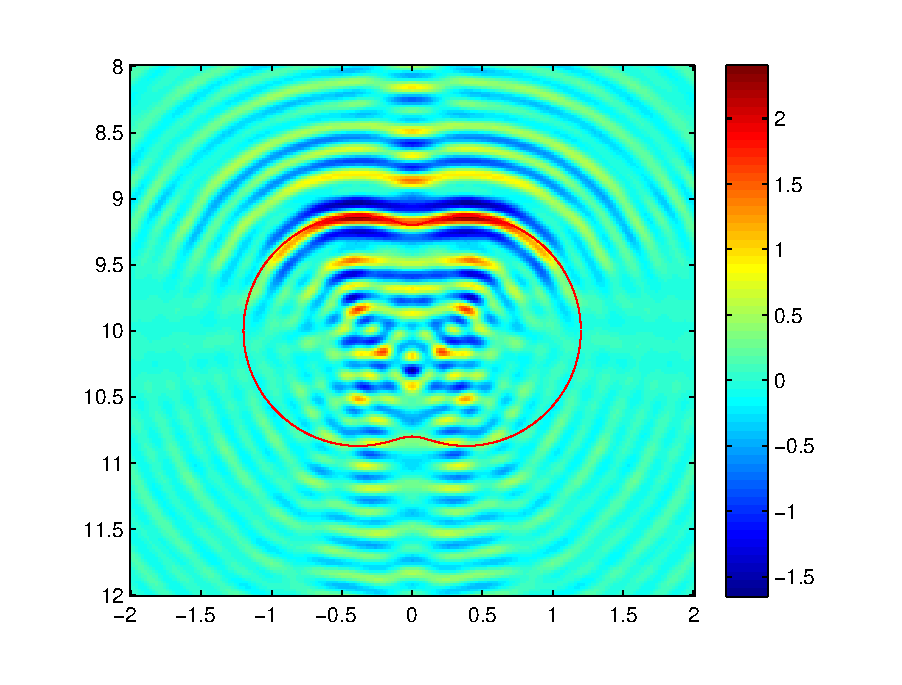
\includegraphics[width=0.24\textwidth]{./Img/graphic/peanut_3pi.eps}
	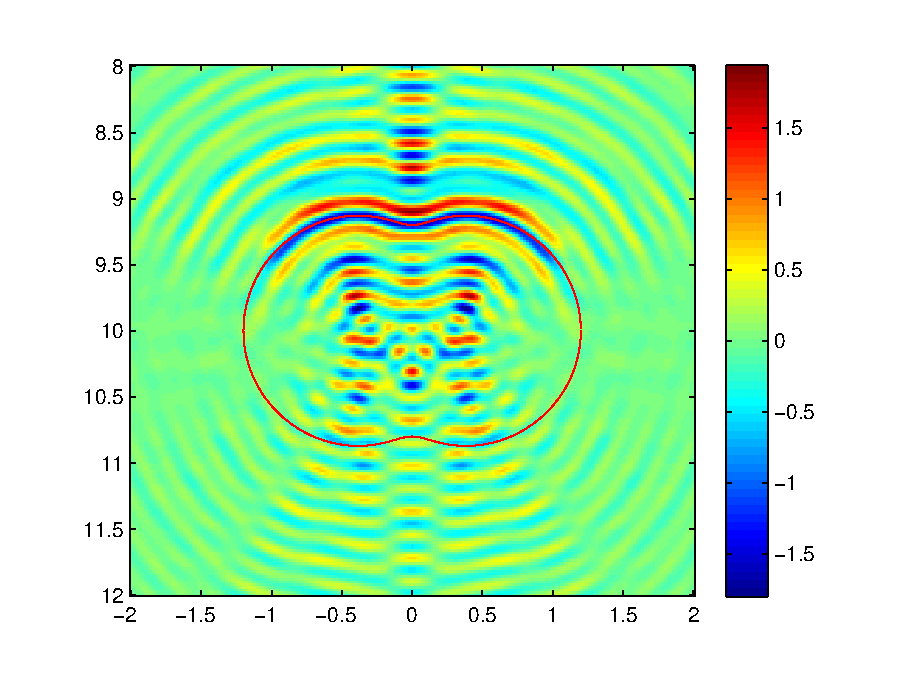
\includegraphics[width=0.24\textwidth]{./Img/graphic/peanut_3pi_neumann.eps}
	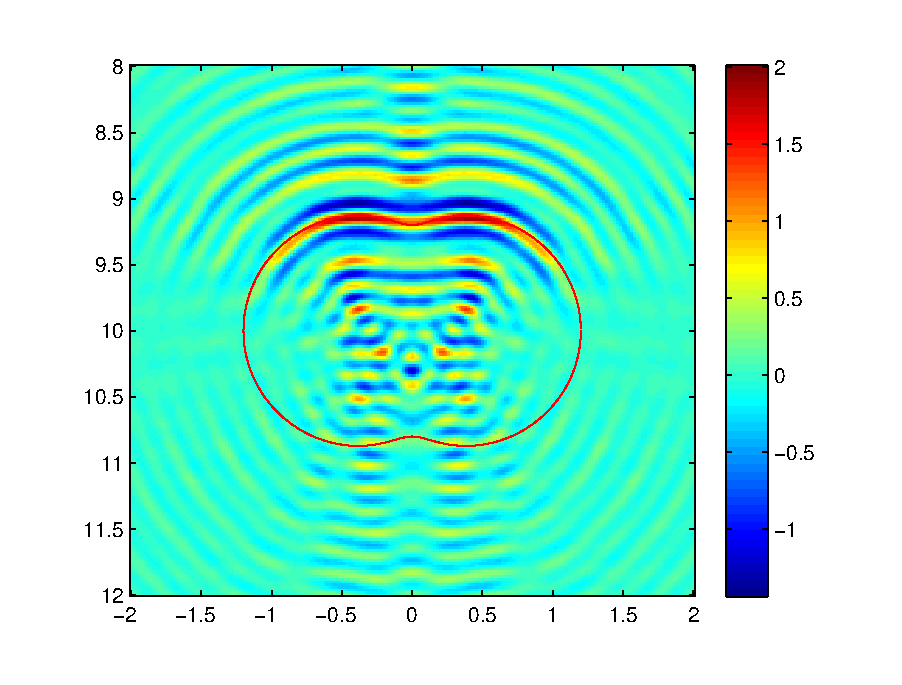
\includegraphics[width=0.24\textwidth]{./Img/graphic/peanut_3pi_impedance_1.eps}
	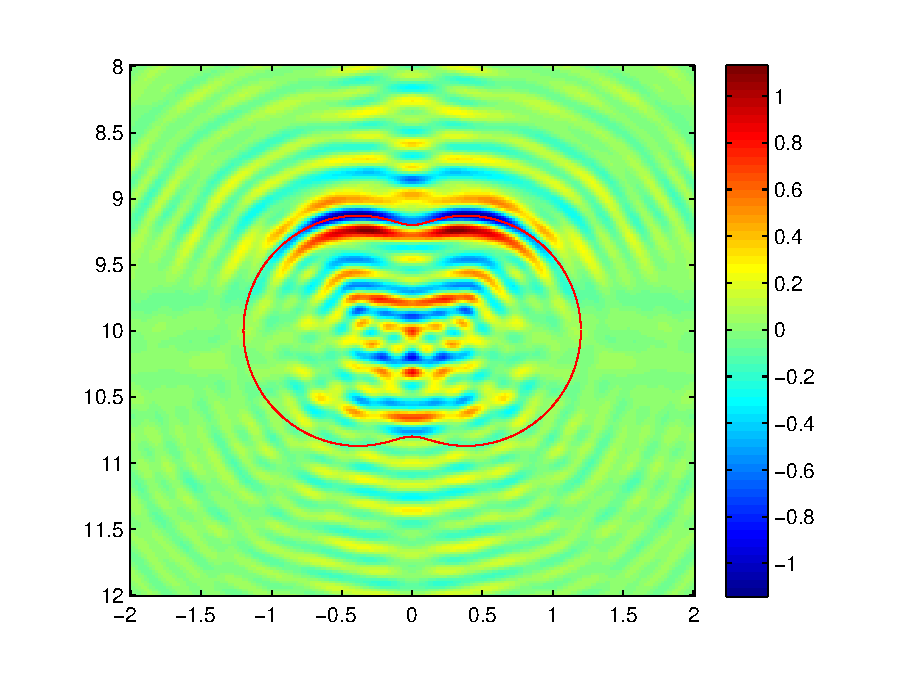
\includegraphics[width=0.24\textwidth]{./Img/graphic/peanut_3pi_transmission.eps}
	\caption{算例 2: 从左到右: Neumann 障碍物, 阻抗障碍物, 以及衍射指数为$n(x)=0.25$
		可穿透障碍物的成像结果} \label{figure_11}
\end{figure}

成像结果见图 \ref{figure_11} 所示。我们可以清晰可见,对于不可穿透障碍物, 障碍物的上边界都被 RTM 方法成像出来,且这部分边界刚好是正对着分布着发射器和接收器的半空间表面 $\Ga_0$,相比较下, 位于障碍物边界的阴暗部分的点以及远离边界的点的成像函数值都是非常小的。

显然, 成像算法(\ref{cor})与障碍是否可穿透, 可穿透时是哪种边界条件无关。在不知道障碍物边界的先验信息下,如图\ref{figure_11}所示,针对不同类型的障碍物, RTM 方法都可以成像。

\bigskip
\textbf{算例 3} 我们考虑来针对两个障碍物同时成像。第一个模型是在水平方向上并排两个障碍物; 第二个模型是一个圆和一个花生在竖直方向上排列 (圆上花生下);第三个模型是一个圆和一个花生在竖直方向上排列 (圆下花生上)。 针对单频的成像实验, 我们取角频率为 $\om=3\pi$ , 而针对多频的成像实验, 我们取多频角频率为 $\om=\pi\times[2:0.5:8]$ 。 如图 \ref{figure_31} 所示,是第一个模型的成像结果。 其成像区域为 $\Om=(-4, 4) \times (8,12)$ , 采样网格点数量 $401 \times 201$。我们设置发射器和接收器数量为 $N_s = N_r = 301$。 如图 \ref{figure_32}和\ref{figure_33} 所示,是第二个模型和第三个模型的成像结果。 其成像区域为 $\Om=(-4, 4)\times (8,12)$ , 采样网格点数量 $401 \times 401$。 我们设置发射器和接收器数量为 $N_s = N_r = 301$。在图 \ref{figure_31} ,图 \ref{figure_32}和图\ref{figure_33} 中的多频 RTM 成像只是简单地将每个不同的单频 RTM 成像结果直接叠加而得。 我们可以发现, 通过这样简单的多个单频叠加后, 成像质量得到显著地提高。
 
\begin{figure}[htbp]
	\centering
	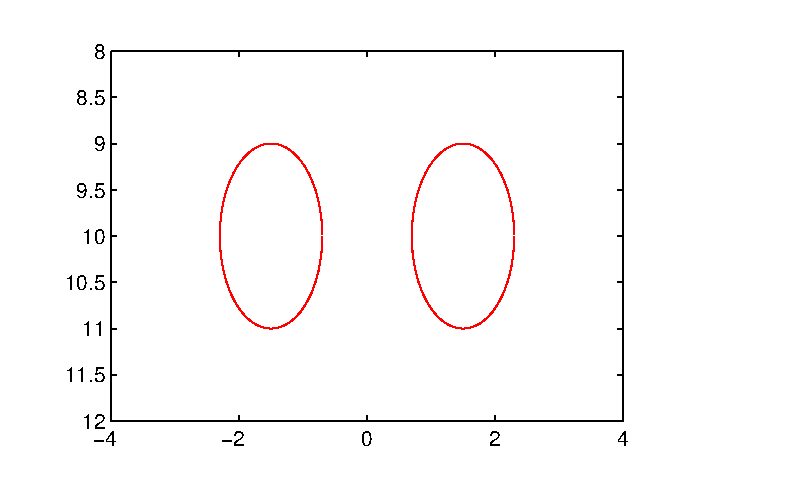
\includegraphics[width=0.32\textwidth,height=0.16\textheight]{./Img/graphic/bi_circle_profile.eps}
	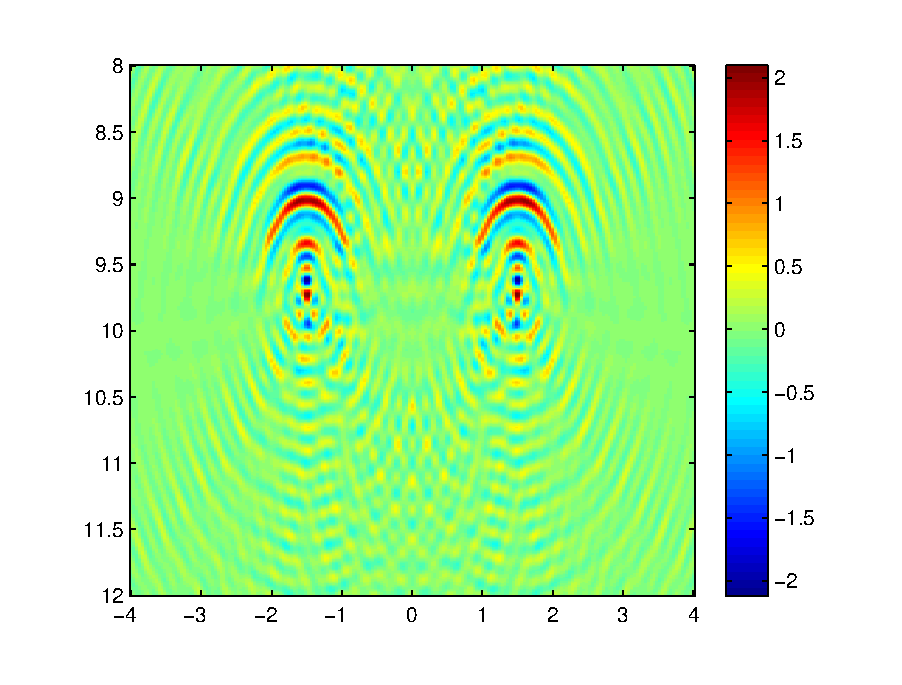
\includegraphics[width=0.32\textwidth]{./Img/graphic/bi_circle_3pi.eps}
	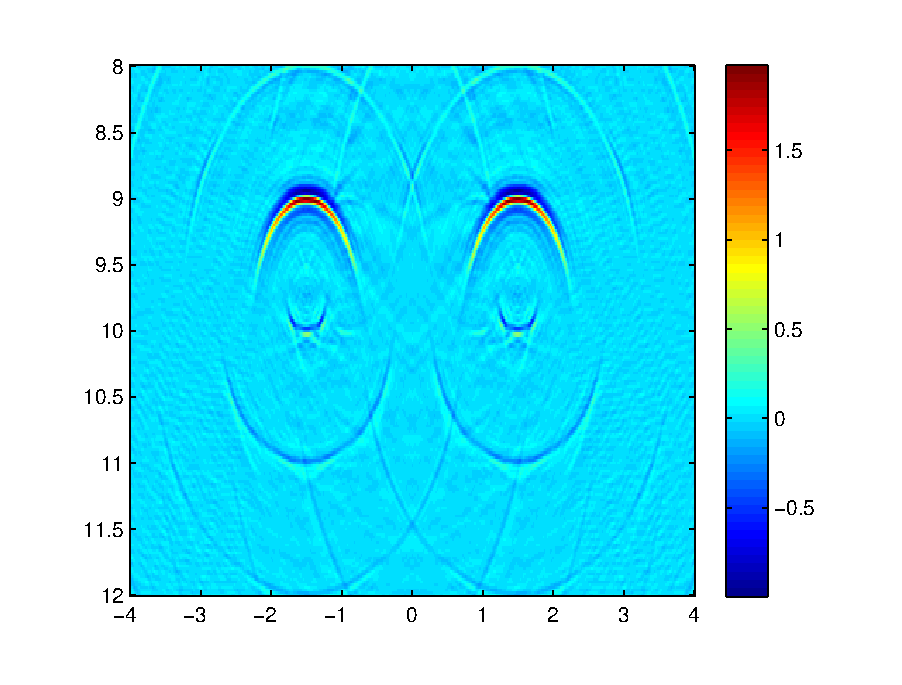
\includegraphics[width=0.32\textwidth]{./Img/graphic/bi_circle.eps}
	
	\caption{算例 3: 从左到右分别为,  真实的两个障碍物:圆, 关于单频角频率为 $\om=3\pi$的成像结果, 关于多频叠加的成像结果。}\label{figure_31}
\end{figure}

\begin{figure}[htbp]
	\centering
	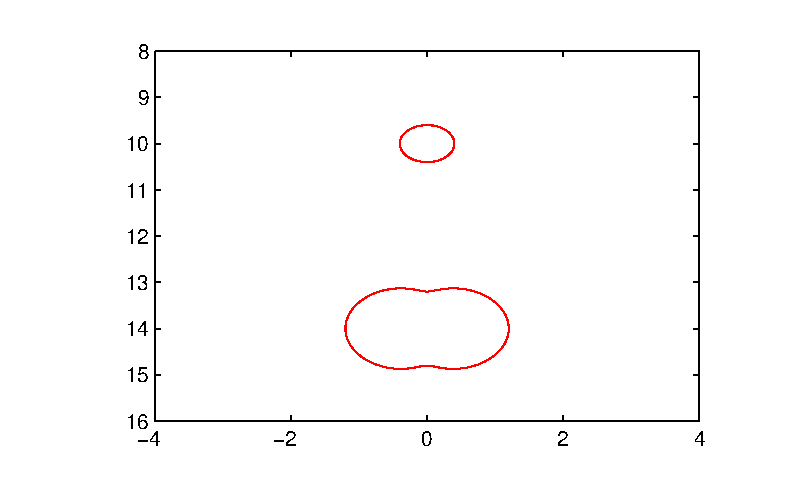
\includegraphics[width=0.32\textwidth,height=0.16\textheight]{./Img/graphic/circle_0_4_peanut_1_profile.eps}
	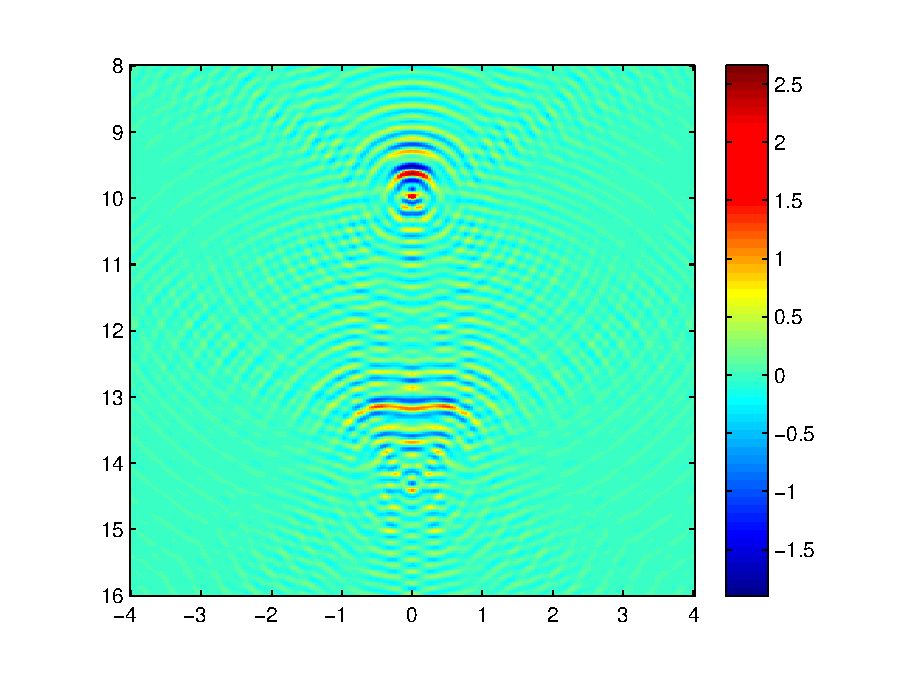
\includegraphics[width=0.32\textwidth]{./Img/graphic/circle_0_4_peanut_1_3pi_1.eps}
	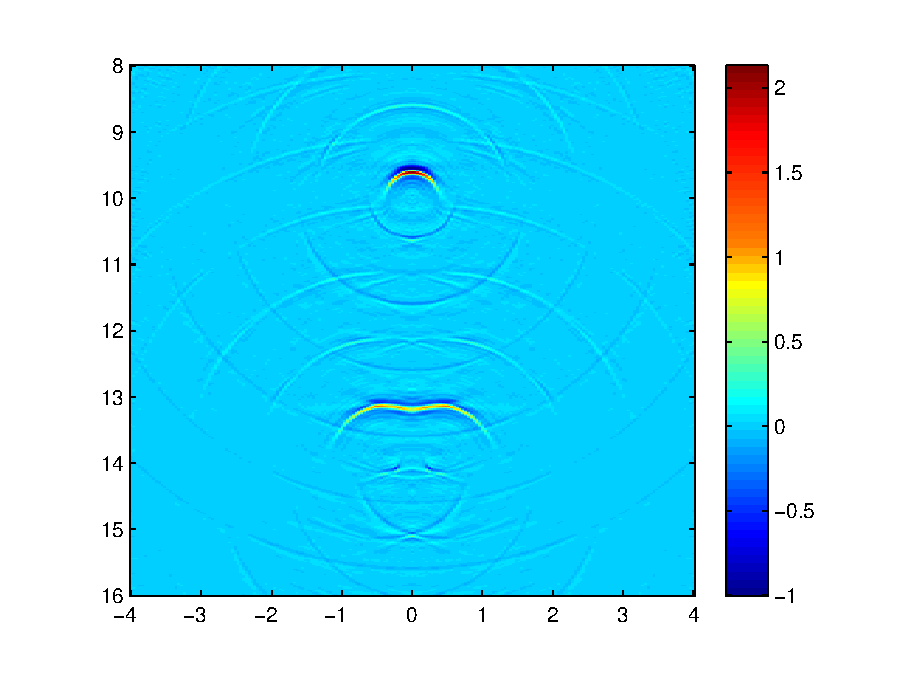
\includegraphics[width=0.32\textwidth]{./Img/graphic/circle_0_4_peanut_1_multi_1.eps}
	
	\caption{算例 3: 从左到右分别为,  真实的两个障碍物:圆上和花生下, 关于单频角频率为 $\om=3\pi$的成像结果, 关于多频叠加的成像结果。}\label{figure_32}
\end{figure}

 如图 \ref{figure_32} 所示, 我们发现即使圆形挡在花生的上面, RTM 算法还是可以将圆和花生的上沿都给成像出来, 进一步说明了 RTM 算法的有效性。而如图 \ref{figure_33} 所示,我们法向当大一号的花生挡在圆的上面时,只能将花生的上沿给成像出来, 而无法对圆成像,我们可以猜测在这种情况下由于花生的阻挡,可能在 $\Ga_0$ 上接受到关于圆的信息是极少的。
\begin{figure}[htbp]
 	\centering
 	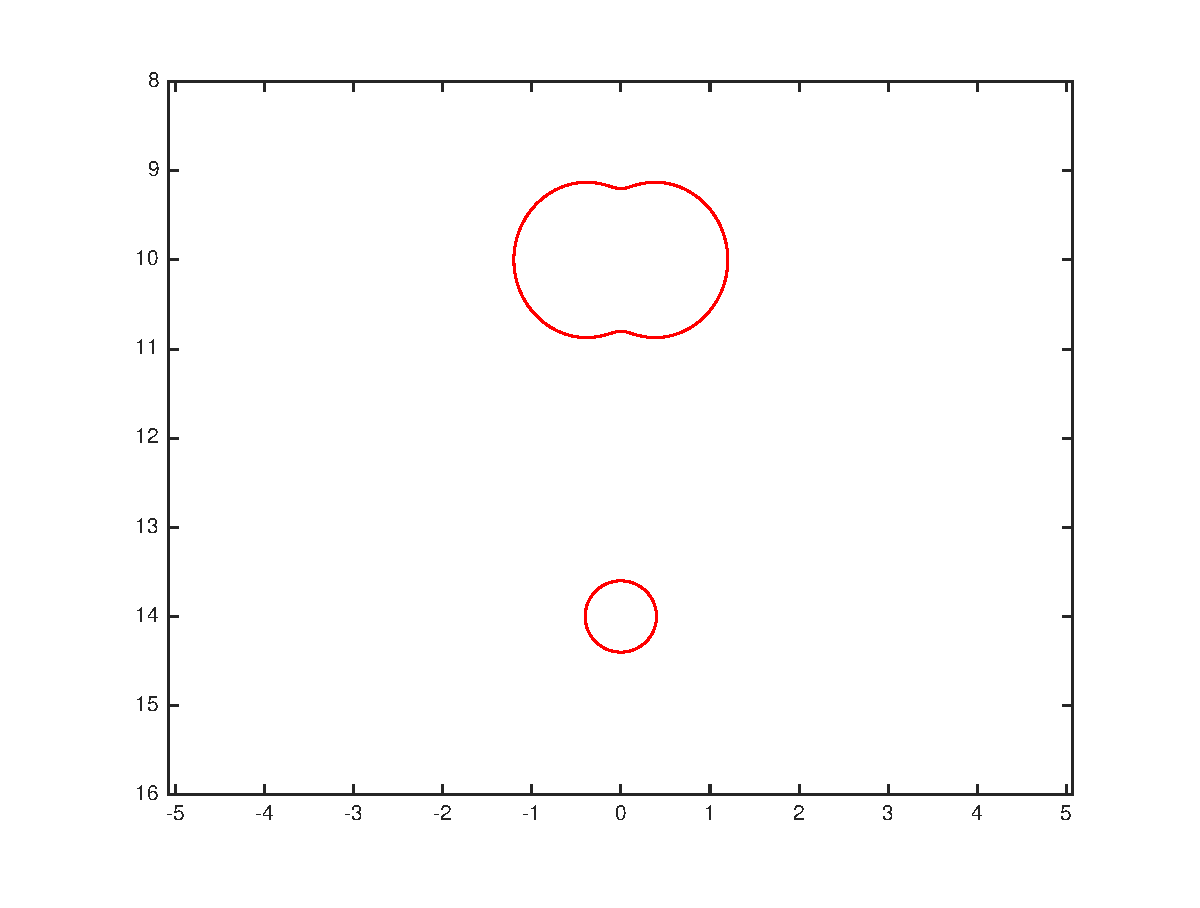
\includegraphics[width=0.32\textwidth,height=0.16\textheight]{./Img/graphic/circle_0_4_peanut_1_profile_reverse.eps}
 	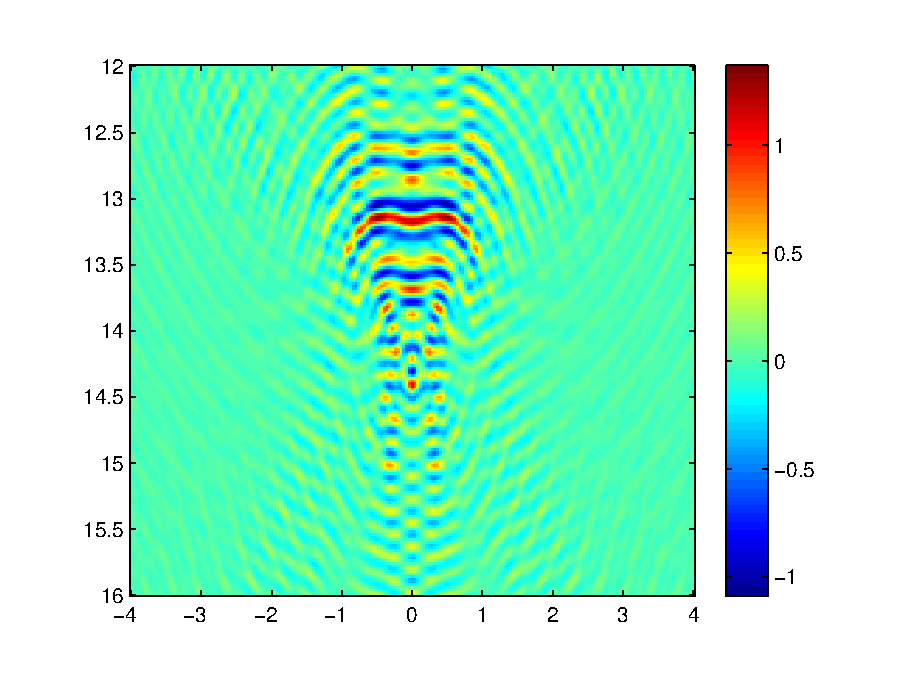
\includegraphics[width=0.32\textwidth]{./Img/graphic/circle_0_4_peanut_1_3pi_down.eps}
 	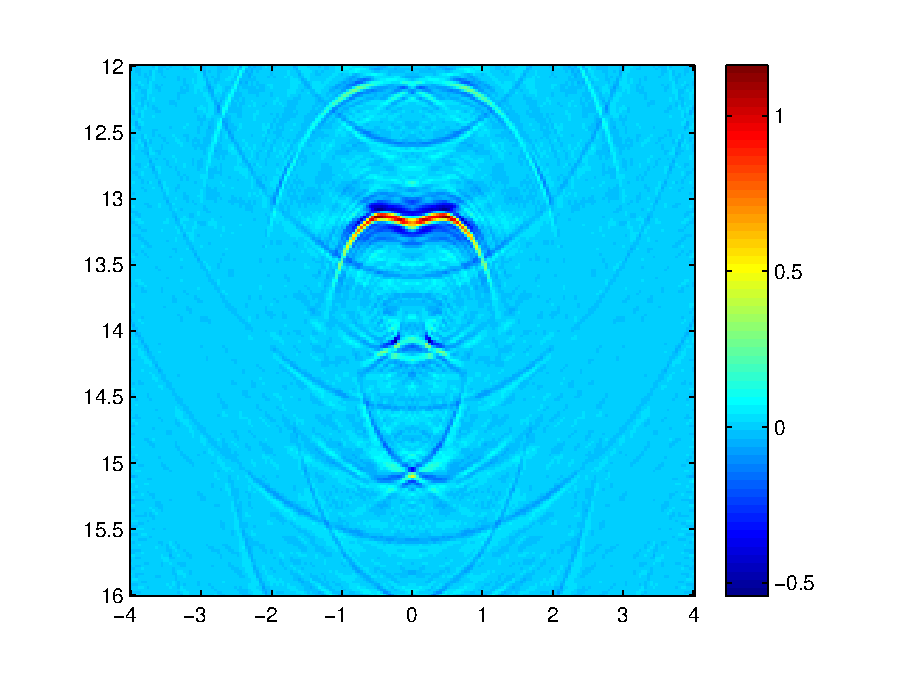
\includegraphics[width=0.32\textwidth]{./Img/graphic/circle_0_4_peanut_1_multi_down.eps}
 	
 	\caption{算例 3: 从左到右分别为,  真实的两个障碍物:圆下和花生上, 关于单频角频率为 $\om=3\pi$的成像结果, 关于多频叠加的成像结果。}\label{figure_33}
 \end{figure}
 
\bigskip
\textbf{Example 4}
我们考虑半空间弹性波 RTM 算法关于复加性 Gaussian 噪声的稳定性。 这里加性 Gaussian 噪声定义为 
\ben
u_{\rm noise}=u_s+\nu_{\rm noise},
\een
其中 $u_s$ 合成的散射数据, $\nu_{\rm noise}$ 是 Gaussian 噪声, 且均值为0, 其标准差是散射数据 $|u_s|$ 中最大值的 $\sigma$ 倍, 即为 $\nu_{\rm noise}=\frac{\sigma \max |u_s|}{\sqrt{2}}(\ep_1+\i\ep_2)$ 和 $\ep_i\thicksim \mathcal{N}(0,1)$。

\begin{figure}[htbp]
	\centering
	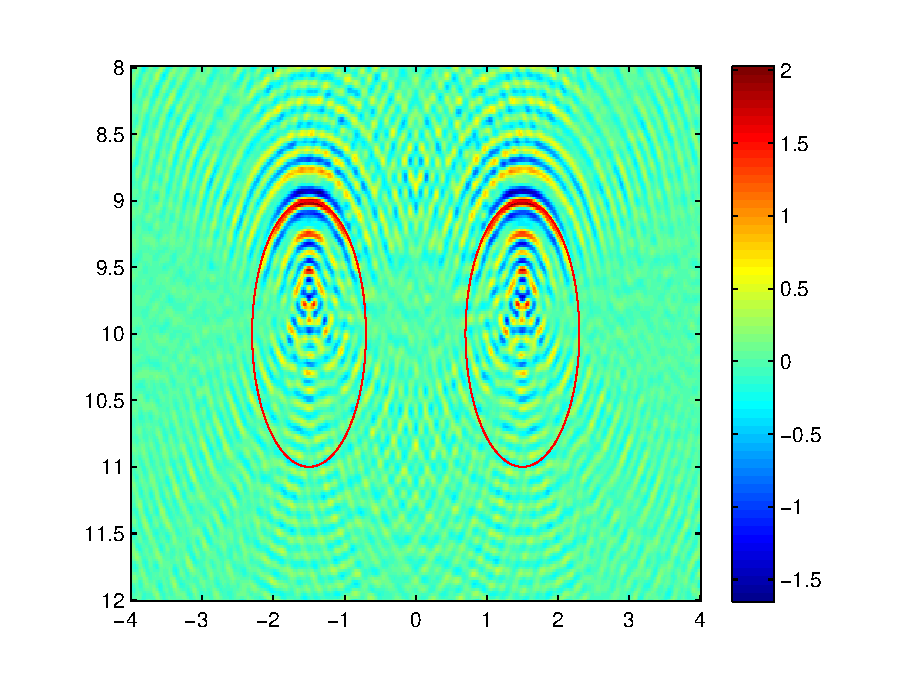
\includegraphics[width=0.32\textwidth]{./Img/graphic/bi_circle_4pi_error2.eps}
	\includegraphics[width=0.32\textwidth]{./Img/graphic/bi_circle_4pi_error4.eps}
	\includegraphics[width=0.32\textwidth]{./Img/graphic/bi_circle_4pi_error6.eps}
	\includegraphics[width=0.32\textwidth]{./Img/graphic/bi_circle_multi_2_8_error2.eps}
	\includegraphics[width=0.32\textwidth]{./Img/graphic/bi_circle_multi_2_8_error4.eps}
	\includegraphics[width=0.32\textwidth]{./Img/graphic/bi_circle_multi_2_8_error6.eps}
	
	\caption{算例 4: 从左到右,分别是含有噪声水平 $\mu =  0.2; 0.3; 0.4$ Dirichlet 障碍物的成像结果。 其中第一行是关于单频成像, 其角频率为 $\om=4\pi$, 第二行是多个单频成像的叠加}\label{figure_4}
\end{figure}

如图 \ref{figure_4} 所示, 即使在加了加性 Gaussian 噪声后, 单频 RTM 成像算法还是可以把障碍物的上沿给清晰成像,说明了该算法的稳定性。  而且在通过多个角频率 $\omega = \pi\times [2:0.5:8]$ 的成像结果叠加后, 其成像质量显著提高,而且消除了 Gaussian 噪声的影响。


\section{本章小结}


\chapter{总结与展望} \label{chap:summary}

本文受地球物理中的勘探模型启发, 针对半空间弹性波反散射问题研究了逆时偏移算法. 在研究反散射问题前, 我们首先系统地研究了半空间弹性波正散射问题.利用 Fourier 变换推导出了两种半空间 Green 函数: Neumann Green 函数和 Dirichlet Green 函数. 进一步, 通过研究振荡积分的衰减性质,给出了当 $x\in \Ga_0, \ y\in \R^2_+$ 时, $\N(x,y)$ 和 $\T_D(x,y)$ 随着 $x_2$ 增大的衰减估计.该估计也保证了点扩散函数的定义有意义.然后, 基于点扩散函数和弹性波散射系数的 Kirchhoff 逼近, 我们针对基于逆时偏移的直接成像法给出了严格的数学刻画: 其成像函数在远离散射体边界的时候快速衰减,且只在散射体面向接收面的那部分形成较大的峰值.而且,该分辨率分析不需要高频渐近假设或几何光学近似,对一般的边界条件都成立. 最后,多种数值算例进一步说明该直接成像法的快速有效性、稳定性.

由于弹性波相较于声波的复杂性,我们将从如下几点来叙述有待研究的方向:

1. 关于 Green 函数的研究

由于半空间的Green 函数都是以震荡积分的形式表述,当频率较大时, 我们需要快速算法来计算. 其中,可否将 Green 函数进行渐近级数展开是一个有趣的问题.本文针对 Green 函数衰减性的研究局限在 $\Ga_0$ 上,将来如果可以将研究范围延拓到半空间上甚至是复数域上, 将有助于对半空间弹性波散射问题的 PML 方法的研究.

 本文中, 我们假设半空间背景介质是均匀各项同性的. 但是实际的地质结构是多层非均匀各向异性的. 针对这种更一般的散射问题,首先需要研究半空间弹性波多层介质的 Green 函数的各种性质,例如合适的表达式、表面波的波数等. 

\bigskip
2. 关于接收数据不是全波位移数据的算法

在实际问题中, 数据的相位可能不好获取, 所以在文献 \cite{chen2016direct,chen2017direct,chen2017phaseless} 中 Chen 等针对声波无相位数据,电磁波无相位数据提出了基于逆时偏移的直接成像法. 由于弹性波数据中横波数据和纵波数据耦合在一起, 所以当只接收到混合波的振幅数据时, 很难效仿上述文献的算法来构造成像函数.本文附录\ref{rtm_phaseless} 中, 我们将不加证明地给出针对全空间弹性波反散射问题的无相位数据的直接成像法及相关数值算法.

进一步,针对真实的勘探模型, 一般 $e_2$ 方向的位移数据更容易得到, 于是如何只用接收到的数据 $u^s_q(x_r,x_s)\cdot e_2, \ q=e_1, \ e_2$ 甚至仅用 $u^s_{e_2}(x_r,x_s)\cdot e_2$ 去成像也是个有意义的研究问题.

\bigskip

3. 关于分辨率分析更严谨的数学刻画

需要通过对点扩散函数更为精确的分析, 得出能分辨出的最小距离 $r$, 即
\ben
r=\inf_{t} \{t=\|z-y\| : |[\J(z,y)]_{ii}|=\frac{1}{2}|[\J(z,z)]_{ii}| ,\ i=1,2\}.
\een
另一方面, 在本文中我们利用了 Kirchhoff 逼近来说明重构算法无法对障碍物的阴面进行成像, 所以对该 Kirchhoff 逼近的误差刻画也是非常重要的一个研究问题.进一步, 本文的直接成像函数只是定性的得到障碍物的性质, 如何通过成像函数得出其边界的参数表达,边界条件类型也是有待研究的.

%---------------------------------------------------------------------------%
% main content
%-
%-> Backmatter: bibliography, glossary, index
%-
\bibliography{Biblio/ref}% bibliography
\end{document}
%---------------------------------------------------------------------------%

